\setlength{\headheight}{24.1278pt}
\linespread{1.6}
\chapter{Introduzione Ambiente distribuito}

L'universo in cui opereremo sarà chiamato \textbf{ambiente di calcolo distribuito}. È costituito da un insieme finito $\epsilon$ di \textbf{entità} computazionali che comunicano per mezzo di \textbf{messaggi}. Le entità comunicano con altre entità per raggiungere un obiettivo comune; ad esempio, per eseguire un determinato compito, per calcolare la soluzione di un problema ecc...

\section{Entità}
L'unità computazionale di un ambiente di calcolo distribuito è chiamata entità. A seconda del sistema modellato dall'ambiente, un'entità può corrispondere a un processo, un processore, uno switch, un agente e così via.

\subsection*{Capabilities}
Ogni entità $x \in \xi$ è dotata di \textbf{memoria locale} (cioè privata e non condivisa) $M_x$. Le capacità di $x$ includono l'\textbf{accesso} (memorizzazione e recupero) alla memoria locale, l'\textbf{elaborazione} locale e la \textbf{comunicazione} (preparazione, trasmissione e ricezione di messaggi). La memoria locale comprende un insieme di registri definiti i cui valori sono sempre inizialmente definiti; tra questi vi sono il \textbf{registro di stato} (indicato con \textit{status(x)}) e il \textbf{registro del valore di input} (indicato con \textit{value(x)}). Il registro \textit{status(x)} assume valori da un insieme finito di stati del sistema $S$; gli esempi di tali valori sono "Idle", "Processing", "Waiting", ecc...\\
Inoltre, ogni entità $x \in \xi$ ha a disposizione una \textbf{sveglia locale o clock} $c_x$ che può impostare e resettare (spegnere).\\
Quindi, riassumendo, un'entità può eseguire solo quattro tipi di operazioni:
\begin{itemize}
    \item memorizzazione ed elaborazione locale
    \item trasmissione di messaggi
    \item impostazione della sveglia
    \item modifica del valore del registro di stato
\end{itemize}

I clock delle entità non sono sincronizzati, pertanto abbiamo un ambiente asincrono. Le entità, in genere, sono alimentate a batteria, e si svegliano solo quando devono fare qualcosa essendo dormienti per la restante parte del tempo.
 
\subsection*{External Events}
Il comportamento di un'entità $x \in \xi$ è \textbf{reattivo}: $x$ risponde solo a stimoli esterni, che chiamiamo \textbf{eventi esterni} (o semplicemente eventi); in assenza di stimoli, $x$ è \textbf{inerte} e non fa nulla. Ci sono tre possibili eventi esterni:
\begin{itemize}
    \item arrivo di un messaggio
    \item suono della sveglia
    \item impulso spontaneo
\end{itemize}

L'arrivo di un \textbf{messaggio} e il suono della \textbf{sveglia} sono eventi esterni all'entità, ma che \textbf{hanno origine all'interno del sistema}: Il messaggio viene inviato da un'altra entità e la sveglia viene impostata dall'entità stessa.\\
A differenza degli altri due tipi di eventi, un \textbf{impulso spontaneo è innescato da forze esterne al sistema} e quindi al di fuori del sistema.

\subsection*{Azioni}
Quando si verifica un evento esterno $e$, un'entità $x \in \xi$ reagisce a $e$ compiendo una sequenza finita, indivisibile e terminante chiamata \textbf{azione}.
Un'azione è indivisibile (o atomica) nel senso che le sue operazioni vengono eseguite \textbf{senza interruzione}; in altre parole, una volta iniziata un'azione, non si fermerà finché non sarà terminata (in un tempo finito).\\
Un'azione speciale che un'entità può intraprendere è l'azione \textit{`nil`}, in cui l'entità non reagisce all'evento.

\subsection*{Comportamento}
La natura dell'azione eseguita dall'entità dipende dalla natura dell'evento $e$, nonché dallo stato in cui si trova l'entità (cioè il valore di `status(x)`) quando si verificano gli eventi. Pertanto, la specifica avrà la forma
$$
Stato \times Evento \rightarrow Azione
$$
che sarà chiamata \textbf{regola}. In una regola $s \times e \rightarrow A$, diciamo che la regola è abilitata da $(s, e)$.\\
Il comportamento, di un'entità $x$ è l'insieme $B(x)$ di tutte le regole a cui $x$ obbedisce. Questo insieme deve essere \textbf{completo e non ambiguo}: per ogni possibile evento $e$ e valore di stato $s$, esiste una e una sola regola in $B(x)$ abilitata da $(s,e)$. In altre parole, $x$ \textbf{deve sempre sapere esattamente cosa deve fare quando si verifica un evento.}\\
L'insieme di regole $B(x)$ è anche chiamato \textbf{protocollo} o \textbf{algoritmo distribuito di $x$}.\\
La specifica comportamentale dell'intero ambiente di calcolo distribuito è solo l'insieme dei comportamenti individuali delle entità. Più precisamente, il \textbf{comportamento collettivo $B(\xi)$} di un insieme $\xi$ di entità è l'insieme $B(\xi) = {B(x): x \in \xi}$.\\
Quindi, in un ambiente con comportamento collettivo $B(\xi)$, ogni entità $x$ agirà (si comporta) secondo il suo algoritmo e protocollo distribuito (insieme di regole) $B(x)$.

\textbf{Un comportamento collettivo è omogeneo se tutte le entità del sistema hanno lo stesso comportamento}, cioè $\forall x, y \in \xi, B(x) = B(y)$.\\
Questo significa che per specificare un comportamento collettivo omogeneo è sufficiente specificare il comportamento di una singola entità, in questo caso, indicheremo il comportamento semplicemente con B. 

Un fatto interessante e importante è il seguente:\\
\textbf{Proprietà 1.1.1} Ogni comportamento collettivo può essere reso omogeneo.\\
Questo significa che se ci troviamo in un sistema in cui entità diverse hanno comportamenti diversi, possiamo scrivere un nuovo insieme di regole, uguale per tutte, che le farà continuare a comportarsi come prima.

\subsection*{Comunicazioni}
In un ambiente informatico distribuito, le entità comunicano \textbf{trasmettendo} e \textbf{ricevendo messaggi}.\\
Nella sua definizione più generale, \textit{un messaggio è solo una sequenza finita di bit}.\\
Un'entità comunica trasmettendo e ricevendo messaggi da altre entità. L'insieme delle entità con cui un'entità può comunicare direttamente non è necessariamente tutto $\xi$; in altre parole, è possibile che un'entità possa comunicare direttamente solo con un sottoinsieme di altre entità.
\begin{itemize}
    \item Denotiamo con $N_{out}(x) \subset \xi$ l'insieme delle entità a cui $x$ può trasmettere direttamente un messaggio; le chiameremo \textit{out-neighbors} di $x$. 
    \item  Allo stesso modo, denotiamo con $N_{in}(x) \subset \xi$ l'insieme delle entità da cui $x$ può ricevere direttamente un messaggio; li chiameremo \textit{in-neighbors} di $x$.
\end{itemize}
 
La relazione di vicinato definisce un grafo diretto $\overrightarrow{G} = (V , \overrightarrow{E})$, dove $V$ è l'insieme dei vertici ed $\overrightarrow{E} \subset V \times V$ è l'insieme degli archi, i vertici corrispondono alle entità e $(x, y) \in \overrightarrow{E}$ se e solo se l'entità (corrispondente a) $y$ è un out-neighbor dell'entità (corrispondente a) $x$.\\
Il grafo diretto $\overrightarrow{G} = (V , \overrightarrow{E})$ descrive la \textbf{topologia di comunicazione} dell'ambiente. Indicheremo con $n(\overrightarrow{G}), m(\overrightarrow{G})$ e $d(\overrightarrow{G})$ il numero di vertici, di archi e il diametro di $\overrightarrow{G}$, rispettivamente. Quando non sorgono ambiguità, ometteremo il riferimento a G e useremo semplicemente $n$, $m$ e $d$.\\\\
In sintesi, un'entità può solo ricevere messaggi dai suoi vicini e inviare messaggi ai suoi out-neighbors.\\
Le entità e le comunicazioni possono fallire.

\section{Assiomi e restrizioni}
La definizione di ambiente di calcolo distribuito con comunicazione punto a punto ha \textbf{due assiomi fondamentali}:
\begin{itemize}
    \item uno sul \textbf{ritardo della comunicazione}
    \item  l'altro sull'\textbf{orientamento locale} delle entità del sistema.
\end{itemize}

Qualsiasi presupposto aggiuntivo (ad esempio, una proprietà della rete, una conoscenza a priori da parte delle entità) sarà chiamato \textbf{restrizione}.

\subsection{Assiomi}
\subsubsection{Communication Delays}
La comunicazione di un messaggio comporta diverse attività: preparazione, trasmissione, ricezione ed elaborazione.\\
L'insieme dei ritardi incontrati da un messaggio sarà chiamato ritardo di comunicazione di quel messaggio.

\textbf{Assioma 1.3.1} Ritardo di comunicazione finito\\
In assenza di guasti, i ritardi di comunicazione sono finiti.

In altre parole, in assenza di guasti, un messaggio inviato a un out-neighbor finirà per arrivare nella sua integrità ed essere elaborato. 

\textbf{Local Orientation}
Un'entità può comunicare direttamente con un sottoinsieme di altre entità: i suoi vicini. L'unico altro assioma del modello è che un'entità può distinguere tra i suoi vicini.

\textbf{Assioma 1.3.2} Orientamento locale\\
\begin{itemize}
    \item Un'entità può distinguere tra i suoi in-neighbors.
    \item Un'entità può distinguere tra i suoi out-neighbors.
\end{itemize}

In particolare, un'entità è in grado di inviare un messaggio solo a uno specifico out-neighbor (senza doverlo inviare anche a tutti gli altri out-neighbor). Inoltre, quando elabora un messaggio (cioè esegue la regola abilitata dalla ricezione di quel messaggio), un'entità può distinguere quale dei suoi in-neighbors ha inviato quel messaggio.

In altre parole, ogni entità $x$ ha una funzione locale $\lambda_x$ che associa etichette, dette anche numeri di porta, ai suoi collegamenti (o porte) incidenti, e questa funzione è iniettiva. Denotiamo i numeri di porta con $\lambda_x (x, y)$, l'etichetta associata da $x$ al collegamento $(x, y)$.\\
Si noti che per ogni arco $(x, y) \in \overrightarrow{E}$, ci sono due etichette: $\lambda_x (x, y)$ locale a $x$ e $\lambda_y (x, y)$ locale a $y$ (si veda la Figura 1.1).\\
A causa di questo assioma, avremo sempre a che fare con \textbf{grafi con archi etichettati} $(\overrightarrow{G}, \lambda)$, dove $\lambda = {\lambda_x : x \in V }$ è l'insieme di queste etichette iniettive.

\begin{figure}[H]
    \centering
    \hspace*{-0.75in}
    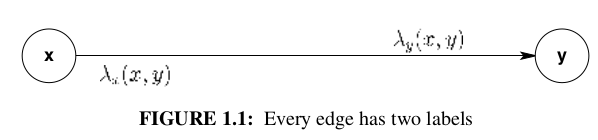
\includegraphics[width=10cm, keepaspectratio]{imgs/img1.png}
\end{figure}

\subsection{Restrizioni}
Le restrizioni possono essere di varia natura e tipo:
\begin{itemize}
    \item possono essere correlate a proprietà di \textbf{comunicazione}, 
    \item \textbf{affidabilità}, 
    \item \textbf{sincronia} e così via.
\end{itemize}

\subsubsection{Restrizioni di Comunicazione}
\textbf{Queueing Policy}: Un collegamento $(x, y)$ può essere visto come un canale o una coda: $x$ invia un messaggio a $y$ equivale a $x$ inserisce il messaggio nel canale.
In generale, sono possibili tutti i tipi di situazioni; ad esempio, i messaggi nel canale potrebbero sovrapporsi e un messaggio successivo potrebbe essere ricevuto per primo.
\begin{itemize}
    \item \textbf{Message Ordering}: In assenza di fallimenti, i messaggi trasmessi da un’entità allo stesso out-neighbor arriveranno nello stesso ordine in cui sono stati inviati.
\end{itemize}

\textbf{Link Property}: Le entità in un sistema di comunicazione sono collegate da collegamenti fisici, che possono avere capacità molto diverse. Gli esempi sono collegamenti simplex e full duplex. Con una linea FULL duplex è possibile trasmettere in entrambe le direzioni.
\begin{itemize}
    \item \textbf{Reciprocal communication:} $\forall x \in \xi, N_{in}(x) = N_{out}(x)$. In altre parole, se $(x, y) \in \overrightarrow{E}$ allora anche $(y, x) \in \overrightarrow{E}$.
    \item \textbf{Bidirectional links}: $\forall x \in \xi, N_{in}(x) = N_{out}(x)$ and $\lambda_x (x, y) = \lambda_x (y,x)$ 
\end{itemize}

\subsubsection{Reliability Restrictions}
\textbf{Detection of Faults}:
\begin{itemize}
  \item \textbf{Edge Failure Detection}: Se il link $(x, y) \in E$ cade, sia $x$ che $y$ rilevano il guasto, e l'eventuale restaurazione;
  \item \textbf{Entity Failure Detection}: $\forall x \in  V$, tutti i $N_{IN}(x)$ e $N_{OUT}(x)$ si accorgono del guasto di $x$ e non usano gli eventuali link. Percepiranno anche quando l'entità è stata riattivata.
\end{itemize}

\textbf{Tipi di guasto}\\
In alcuni sistemi possono verificarsi solo alcuni tipi di guasti: ad esempio, i messaggi possono essere persi ma non danneggiati. Ogni situazione darà luogo a una restrizione corrispondente. Restrizioni più generali descriveranno sistemi o situazioni in cui non ci saranno guasti:
\begin{itemize}
  \item \textbf{Garanzia di consegna:} Ogni messaggio inviato sarà ricevuto con il suo contenuto intatto (non corrotto).
  \item \textbf{Affidabilità parziale}: nessun guasto si verifica durante l'esecuzione dell'algoritmo.\\
  Se $j$ è l'istante in cui inizia il protocollo si assume che nessun guasto si verifica dopo $j$;
  \item \textbf{Affidabilità totale}: Nessun guasto si verifica o si è verificato.
\end{itemize}

\subsubsection{Restrizioni sulla topologia di G}
In generale, un'entità non è direttamente collegata a tutte le altre entità; potrebbe ancora essere in grado di comunicare informazioni a un'entità remota, utilizzando altri come relayer. Un sistema che fornisce questa funzionalità per tutte le entità è caratterizzato dalla seguente restrizione:
\begin{itemize}
    \item \textbf{ Connettività:} La topologia di comunicazione del grafo G è fortemente connessa. Questo significa che ogni entità è possibile raggiungere qualsiasi altro vertice.
\end{itemize}

\subsubsection{Restrizioni sul tempo}
\begin{itemize}
    \item \textbf{Ritardo di comunicazione limitato:} Esiste una costante $\delta$ tale per cui, in assenza di fallimenti, il ritardo di comunicazione di un qualsiasi messaggio, su un qualsiasi collegamento è al più $\delta$.
    \item \textbf{Ritardo di comunicazione unitario:} In assenza di fallimenti, i ritardi di comunicazione di un messaggio su un qualsiasi link richiedono una singola unità di tempo (è un caso speciale del ritardo di comunicazione limitato).
    \item \textbf{Sincronia di clock}: Tutti i clock sono simultaneamente incrementati di un'unità e l'intervallo di tempo tra i successivi incrementi è costante (è il caso generale e non fa assunzioni sui clock locali). 
\end{itemize}

\subsection{Restrizioni di conoscenza}
Riguardano la conoscenza delle singole entità, relativamente ad alcuni parametri. \\ 
Le restrizioni determinano i protocolli di comunicazione, ed in particolare riguardano:
\begin{itemize}
  \item numero di nodi: $|V| = n$ (si può considerare anche una stima di $|V|$);
  \item numero di archi: $|E| = m$;
  \item diametro: $d(G)$;
  \item restrizioni topologiche (ad esempio, possiamo assumere che $G$ è un albero o un ring);
  \item conoscenza di $G$: ogni entità ha una mappa. \\ Si può considerare una conoscenza limitata del grafo. Mediante le assunzioni possiamo fare ad esempio delle implicazioni, cioè se $G$ è completo e ci sono $k$ vicini, allora $|V| = n = k+1$ nodi;
  \item restrizioni \textit{D-type}: i dati dell'entità (ad esempio, ogni entità ha associato un identificatore unico);
  \item restrizioni \textit{L-type}: gli stati interni dell'entità (ad esempio, un unico leader).
\end{itemize}

\section{Costo e Complessità}
Per andare a calcolare il costo di un protocollo prenderemo in considerazione due parametri:
\begin{itemize}
    \item \textit{amount of communication activities}
    \item \textit{time} richiesto dall'esecuzione di una computazione
\end{itemize}

\subsection{Amount of Communication Activities}
La trasmissione di un messaggio attraverso un out-port (cioè a un out-neighbor) è l'attività di comunicazione di base nel sistema; si noti che la trasmissione di un messaggio che non sarà ricevuto per guasto costituisce comunque un'attività di comunicazione.
\begin{itemize}
  \item \textbf{Numero di messaggi $M$} o \textbf{Message cost}: Quanto traffico è generato da questa esecuzione e quanto sarà occupato il sistema? (la funzione più comunemente utilizzata)
  \item Altre funzioni utilizzate sono:
  \begin{itemize}
    \item \textbf{Entity workload}: $L_{NODE} = M / |V|$, media di messaggi spediti da un'entità;
    \item \textbf{Trasmission load}: $L_{LINK} = M / |E|$, media di messaggi su un arco.
  \end{itemize}
 \end{itemize}

I messaggi sono sequenze di bit, più grandi o più piccoli in base al protocollo. È necessario definire un costo per misurare il numero di bits trasmessi, quest'ultimo è chiamato \textbf{B (bit complexity)}.\\
Altre funzioni di carico basate sul bit per misurare il costo:
\begin{itemize}
    \item \textbf{Entity bit-workload}: $Lb_{NODE} = B / |V|$, numero di bits per entità
    \item \textbf{Trasmission bit-load}: $Lb_{LINK} = B / |E|$, numero di bits per link 
\end{itemize}

\subsection{Tempo}
I ritardi nella comunicazione sono imprevedibili.\\
\textbf{Total execution delay}: misura il ritardo tra il tempo che la prima entità impiega a iniziare l'esecuzione e il tempo che l'ultima entità impiega a terminare l'esecuzione.\\
Possiamo misurare il tempo di esecuzione in particolari condizioni:
\begin{itemize}
    \item \textbf{$T$}: \textit{ideal execution delay o ideal time complexity}, è il tempo di esecuzione riscontrato sotto le restrizioni di "\textit{Unitary Transmission Delays}" e "\textit{Synchronized Clocks}"; il sistema è sincrono e impiega un'unità di tempo per trasmettere un messaggio ed elaborarlo
    \item \textbf{$T_{Casual}$}: \textit{Casual time complexity}, è la lunghezza della catena più lunga di trasmissioni casuali di messaggi affidabilit, fra tutte le possibili esecuzioni.
\end{itemize}

\section{Stati ed Eventi}
 Una volta definito il comportamento delle entità, la loro topologia di comunicazione e l'insieme delle restrizioni sotto cui operano, dobbiamo descrivere le condizioni iniziali del nostro ambiente. Questo viene fatto innanzitutto specificando la \textbf{condizione iniziale} di tutte le entità:\\
Il contenuto iniziale di tutti i registri dell'entità $x$ e il valore iniziale della sua sveglia $c_x$ all'istante $t$ costituisce lo \textbf{stato interno iniziale} $\sigma (x, 0)$ di $x$.\\
Sia $\sum(0) = {\sigma (x, 0) : x \in \xi}$ l'insieme di tutti gli stati interni iniziali.\\
Una volta definito $\sum(0)$, abbiamo completato la \textbf{specifica statica dell'ambiente}: la descrizione del sistema prima che si verifichi qualsiasi evento e prima che abbia luogo qualsiasi attività.\\
Siamo, comunque, interessati anche a descrivere il sistema \textbf{durante} le attività computazionali, così come \textbf{dopo} tali attività. Per farlo, dobbiamo essere in grado di descrivere i cambiamenti che il sistema subisce nel tempo. Come accennato in precedenza, le entità (e, quindi, gli ambienti) sono reattive. Cioè, qualsiasi attività del sistema è determinata interamente dagli eventi esterni. Esaminiamo questi fatti in modo più dettagliato.

\subsection{Tempo ed Eventi}
Negli ambienti di elaborazione distribuiti, esistono solo tre tipi di eventi esterni: \textbf{impulso spontaneo, ricezione di un messaggio e suono della sveglia (when)}.\\
Quando un evento esterno si verifica in un'entità, innesca l'esecuzione di un'azione (la natura dell'azione dipende dallo stato dell'entità quando si verifica l'evento). L'azione eseguita può generare nuovi eventi: l'operazione \textbf{send} genererà un evento di ricezione e l'operazione \textbf{set\_alarm} genererà un evento when.\\
Si noti innanzitutto che gli eventi così generati potrebbero non verificarsi affatto. Ad esempio, un errore di collegamento può distruggere il messaggio in viaggio, distruggendo il corrispondente evento di ricezione; in un'azione successiva, un'entità può disattivare l'allarme precedentemente impostato distruggendo l'evento when.\\
Si noti ora che se si verificano, questi eventi lo faranno in un secondo momento (ad esempio, quando arriva il messaggio, quando suona l'allarme). Questo ritardo potrebbe essere noto proprio nel caso della sveglia (perché impostata dall'ente); è invece imprevedibile nel caso di trasmissione di messaggi (perché dovuta a condizioni esterne all'entità). Diversi ritardi danno luogo a diverse esecuzioni degli stessi protocolli con possibili esiti diversi.

Riassumendo, ogni evento $e$ viene “generato” in un istante $t(e)$ e, se si verifica, accadrà in un istante successivo.\\
Per definizione, tutti gli impulsi spontanei sono già generati prima dell'inizio dell'esecuzione; il loro insieme sarà chiamato l'\textbf{insieme degli eventi iniziali}. L'esecuzione del protocollo inizia quando effettivamente si verificano i primi impulsi spontanei; per convenzione, questo sarà il tempo $t = 0$.

\textbf{IMPORTANTE}: Si noti che il "tempo" è qui considerato come visto da un osservatore esterno ed è visto come tempo reale. Ogni istante in tempo reale t separa l'asse del tempo in tre parti: passato (cioè {$t' < t$}), presente (cioè $t$) e futuro (cioè {$t' > t$}). Tutti gli eventi generati prima di $t$ che accadranno dopo $t$ sono chiamati \textit{future at t} e denotati da \textbf{Future(t)}; rappresenta l'insieme di eventi futuri determinati dal'esecuzione fino a quel momento.

\subsection*{Time Event Diagram (TED)}
Un'esecuzione è descritta dalla sequenza degli eventi che accadono. Per piccoli sistemi, un'esecuzione può essere visualizzata dal diagramma TED. Questo è composta da una linea temporale per ogni entità in $\xi$, su cui indichiamo gli istanti temporali in cui avvengono gli eventi.
\begin{center}
  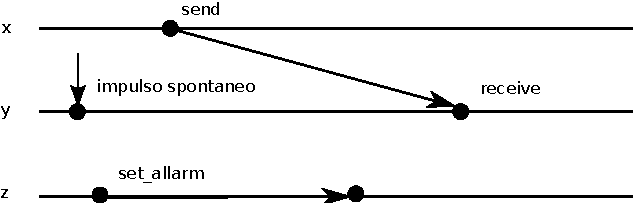
\includegraphics[scale=0.8]{images/n_07}
\end{center}

\begin{itemize}
    \item \textbf{Evento di ricezione}: Rappresentato da una freccia che va da x ad y.
    \item \textbf{Evento di ring dell'allarme (when)}: Rappresentata da una freccia dal punto t' al punto t''
    \item \textbf{Evento spontaneo}: rappresentato da una piccola freccia che indica il punto t nella linea temporale dell'entità $x$ in cui l'evento avviene
\end{itemize}

Per convenzione, l'inizio del protocollo è dato dall'istante in cui si verifica il primo impulso spontaneo. Infatti $t=0$ corrisponde al momento in cui il primo impulso spontaneo si verifica:
\begin{center}
  \texttt{eventi\_iniziali} $=\lbrace$ impulsi spontanei $\rbrace$
\end{center}
Ci possono essere degli eventi \textbf{contemporanei} per cui impostiamo delle precedenze, come:
\begin{center}
  \texttt{spontaneously} $\geq$ \texttt{sveglia} $\geq$ \texttt{receiving}
\end{center}

\subsection{Stati e Configurazioni}
La memoria privata di ogni entità, oltre al comportamento, contiene un insieme di registri, alcuni già inizializzati, altri da inizializzare durante l'esecuzione.\\
Il contenuto di tutti i registri dell'entità $x$ e il valore della sua sveglia $c_x$ all'istante $t$ costituiscono quello che viene chiamato lo stato interno di $x$ in $t$ ed è indicato con $\sigma (x, t)$. Indichiamo con $\sum(t)$ l'insieme degli stati interni al tempo $t$ di tutte le entità. Gli stati interni cambiano con il tempo e il verificarsi di eventi.\\
C'è un fatto importante sugli stati interni. Consideriamo due ambienti diversi, $E_1$ ed $E_2$ , dove, per caso, lo stato interno di $x$ all'istante $t$ è lo stesso. Quindi $x$ non può distinguere tra i due ambienti, cioè $x$ non è in grado di dire se si trova nell'ambiente $E_1$ o $E_2$.\\
C'è una conseguenza importante. Consideriamo la situazione appena descritta: all'istante $t$, lo stato interno di $x$ è lo stesso sia in $E_1$ che in $E_2$. Supponiamo ora che, anche per caso, si verifichi esattamente lo stesso evento in $x$ (ad esempio, la sveglia suona o lo stesso messaggio viene ricevuto dallo stesso vicino). Quindi $x$ eseguirà esattamente la stessa azione in entrambi i casi e il suo stato interno continuerà ad essere lo stesso in entrambe le situazioni.

\properties[1.6.1]{
  Assumendo che lo stesso evento si verifica in $x \in  \xi$ al tempo $t$ in due differenti esecuzioni, e siano $\sigma_1$ e $\sigma_2$ gli stati interni di $x$ quando ciò si verifica, allora se $\sigma_1 = \sigma_2$, il nuovo stato interno di $x$ sarà lo stesso in entrambe le esecuzioni.\\ Un'entità non riesce a distinguere tra le esecuzioni.
}

\properties[1.6.2]{
  Assumendo che lo stesso evento si verifica in $x$ e $y$ al tempo $t$ e siano $\sigma_1$ e $\sigma_2$ i rispettivi stati interni, allora se $\sigma_1 = \sigma_2$ lo stato interno di $x$ e $y$ sarà ancora lo stesso. Dall'esterno non riusciamo a distinguere tra le entità.
}

Lo stato globale di un sistema si può rappresentare mediante la \textbf{configurazione} della rete al tempo $t$:
\begin{center}
  \texttt{C(t) = $(\Sigma(t)$, \texttt{Future(t)})}
\end{center}
dove:
\begin{itemize}
    \item $\sum(t)$ specifica lo stato interno di tutte le entità a tempo $t$.
    \item \texttt{Future(t)} è l'insieme di tutti gli eventi che si verificheranno a tempo $t$. Quindi se $future(t) = 0$ significa che non si dovranno generare più eventi.
\end{itemize}

La configurazione iniziale $C(0)$ contiene non solo l'insieme iniziale degli stati $(0)$ ma anche l'insieme $Future(0)$ degli impulsi spontanei. Gli ambienti che differiscono solo nella loro configurazione iniziale verranno chiamati istanze dello stesso sistema.\\
La configurazione $C(t)$ è come un'istantanea del sistema all'istante $t$.


\section{Definizione formale di un problema}
Un algoritmo distribuito è l'insieme di regole che definiscono i comportamenti delle entità. Il motivo per cui potremmo aver bisogno di progettare i comportamenti è consentire alle entità di risolvere un determinato problema, eseguire un'attività definita o fornire un servizio richiesto.
In generale, ci verrà dato un problema e il nostro compito è progettare un insieme di regole che risolveranno sempre il problema in un tempo finito.

\definition{
  Un problema $P$ è definito dalla terna:
  \begin{eqnarray}
    P = P_{INIT}, P_{FINAL}, R
    \nonumber
  \end{eqnarray}
  dove:
  \begin{itemize}
    \item $P_{INIT}$ è un predicato che specifica le condizioni iniziali;
    \item $P_{FINAL}$ è un predicato che specifica le condizioni finali;
    \item $R$ è l'insieme delle restrizioni.
  \end{itemize}}

\example{
  \texttt{Broadcast}:
  \begin{itemize}
    \item $P_{INIT}$ = ``Solo un'entità ha l'informazione $I$ al tempo $t=0$'':
    \begin{center}
      $(\exists x \in \xi : \textrm{value}_t(x) = I) ~~ \wedge ~~ (\forall y \neq x \in \xi,~\textrm{value}_t(y) = \emptyset)$
    \end{center}
    
    \texttt{Future(t)} = $i$ su $x$ ($i$ rappresenta l'impulso spontaneo su $x$).
    
    \item $P_{FINAL}$ = ``Tutte le entità hanno l'informazione $I$ al tempo $t$'':
    \begin{center}
      $\forall x \in \xi : \textrm{value}_t(x) = I$ 
    \end{center}
    
    \item $R$ = Affidabilità totale; connettività; link bidirezionali.
  \end{itemize}

}

\subsection{Stati}
Sia $B$ un protocollo che da la soluzione al problema P=$<P_{init}, P_{final}, R>$. Parte di definizione del protocollo deve essere svolta dalla definizione degli insiemi degli stati.
\begin{itemize}
  \item $S_{INIT}$: stati iniziali di tutte le entità all'inizio del protocollo (es: initiator, idle);
  \item $S_{TERM}$: stati terminali, una volta che questi stati sono raggiunti non potranno mai essere cambiati dal protocollo (es: done);
  \item $S_{INTERMEDI}$: Stati ne finali ne iniziali.
\end{itemize}

Gli stati iniziali e terminali sono, a loro volta, divisi in:
\begin{itemize}
  \item $S_{START}\subseteq S_{INIT} \Rightarrow$ Stati che danno inizio al protocollo (quindi quelli che possono ricevere l'impulso spontaneo).
  \item $S_{FINAL}\subseteq S_{TERM} \Rightarrow$ Le entità in $S_{FINAL}$ non eseguono più azioni, ovvero processano solo $nil$. Le entità in questi stati non possono comunque cambiare stato, poichè questo insieme è incluso in quelli terminali $S_{TERM}$.
\end{itemize}

Quindi si avrà che $S: S_{INIT} \cup S_{TERM} \cup S_{INTERMEDI}$

\subsection{Terminazione}
Un protocollo $B$ termina se per tutte le configurazioni iniziali $C(0)$ che soddisfano $P_{INIT}$ e per tutte le esecuzioni che partono da tali configurazioni il predicato 
\begin{center}
    $\texttt{Terminate(t)} \equiv (\{STATUS_t\} \subseteq S_{TERM} \; \wedge \; \texttt{Future(t)} = \emptyset) \;$ vale per qualche \; $t>0$,
\end{center}
cioè tutte le entità entrano in uno stato terminale dopo un tempo finito e tutti gli eventi generati si sono verificati.Quindi se tutte le entità entrano in uno stato terminale dopo un certo tempo finito $t$ e tutti gli eventi generati si sono verificati.\\
Un'entità non è a conoscenza di quando la terminazione avviene, in generale vorremmo che ogni entità conosca almeno la terminazione locale. Questa situazione è chiamata Explicit\_Termination e si verifica quando il predicato

\begin{center}
    $\texttt{Explicit\_Terminate(t)} \equiv (\{STATUS_t\} \subseteq S_{FINAL}) \;$ vale per qualche $t>0$
\end{center}
Quindi la terminazione esplicita avviene quando tutte le entità entrano in uno stato finale dopo un tempo finito.

%\textbf{Mio Terminazione:} Un protocollo B termina se per tutte le configurazioni iniziali $C(0)$ che soddisfano $P_{init}$ dopo un tempo finito tutte le entità entrano in stato Terminale e non si verificheranno più eventi, poichè $future(t)$ è vuoto.\\
%\textbf{Mio Terminazione\_Esplicita:}  Vogliamo che tutte le entità siano a conoscenza ALMENO della terminazione locale, per far questo quindi viene utilizzato l'insieme degli stati $S_{FINAL}$. Questa accade quando lo stato di un'entità è incluso in quell'insieme.

\subsection{Correttezza}
\definition{
  Un protocollo $B$ è \textbf{corretto} se per tutte le esecuzioni che partono da una configurazione iniziale che soddisfa $P_{INIT}$:
  \begin{center}
    $\exists t>0$ tale che vale $Correct(t)$ dove $Correct(t) \equiv \forall t' \geq t$ vale $P_{FINAL}(t')$,
  \end{center}
}
dove $Correct(t) \equiv (\forall t' \ge t, P_{FINAL}(t)$); cioè, il predicato finale alla fine vale e non cambia. 

\subsection{Soluzione}
 L'insieme di regole $B$ \textbf{risolve} il problema $P$ se termina sempre correttamente sotto le restrizioni $R$. Dato che abbiamo due tipi di terminazione, abbiamo anche due tipi di soluzione:
  \begin{itemize}
    \item \texttt{Simple\_solution(B, P)} = $\exists t > 0 :$ \texttt{Correct(t)} $ ~~ \wedge ~~$ \texttt{Terminate(t)}\\
    Ovvero che il predicato simple solution vale sotto le restrizioni R per ogni esecuzione che inizia da una configurazione iniziale che soddisfa $P_{init}$.
    
    \item \texttt{Explicit\_solution(B, P)} = $\exists t > 0 :$ \texttt{Correct(t)} $ ~~ \wedge ~~$ \texttt{Explicit\_Terminate(t)}\\
        Ovvero che il predicato explicit solution vale sotto le restrizioni R per ogni esecuzione che inizia da una configurazione iniziale che soddisfa $P_{init}$.
  \end{itemize}

% -------------------------------------------

\chapter{Broadcast}
Chiariamo con un esempio i concetti fin qui espressi. Considera un sistema informatico distribuito in cui un'entità ha alcune informazioni importanti sconosciute agli altri e vorrebbe condividerle con tutti gli altri.
Questo problema si chiama \textbf{broadcasting} e fa parte di una classe generale di problemi chiamati \textbf{diffusione dell'informazione}. Risolvere questo problema significa progettare un insieme di regole che, una volta eseguite dalle entità, porteranno (entro un tempo finito) a tutte le entità a conoscere le informazioni; la soluzione deve funzionare indipendentemente da quale entità aveva le informazioni all'inizio.

Quindi:
\begin{itemize}
    \item $P_{INIT}$ = ``Solo un'entità ha l'informazione $I$ al tempo $t=0$'':
    \begin{center}
      $(\exists x \in \xi : \textrm{value}_t(x) = I) ~~ \wedge ~~ (\forall y \neq x \in \xi,~\textrm{value}_t(y) = \emptyset)$
    \end{center}
    \item $P_{FINAL}$ = ``Tutte le entità hanno l'informazione $I$ al tempo $t$'':
    \begin{center}
      $\forall x \in \xi : \textrm{value}_t(x) = I$ 
    \end{center}
\end{itemize}

\textbf{Quindi}: Un'entità si sveglia tramite impulso spontaneo, ha un'informazione non conosciuta dalla altre e vuole informarle tutte.

\section{Restrizioni}
Sia $\xi$ l'insieme delle entità e $G$ la topologia di comunicazione.\\
L'insieme delle restrizioni $R$ è così composto:
\begin{itemize}
  \item \colorbox{yellow}{Link bidirezionali:} grafo non orientato;
  \item \colorbox{yellow}{Affidabilità totale:} non consideriamo guasti di link e/o nodi;
  \item \colorbox{yellow}{Connettività:} grafo connesso, e quindi tutti possono raggiungere tutti;
\end{itemize}

Inoltre si ha la situazione dell'\textbf{Iniziatore Unico}: una sola entità inizialmente è attiva.

\section{Protocollo Broadcast [Senza terminazione]}
L'idea è quella che \colorbox{yellow}{se un'entità ha l'informazione $I$, allora la trasmette a tutti i suoi vicini.} \\ Dobbiamo specificare il \textbf{behavior} tramite la funzione:
\begin{eqnarray}
  S \times E \rightarrow A
  \nonumber
\end{eqnarray}
\begin{itemize}
  \item $S=\lbrace$ \texttt{initiator}, \texttt{idle} $\rbrace$
  \item $E=\lbrace$ \texttt{receiving}, \texttt{alarm}, \texttt{spontaneously=I} $\rbrace$
\end{itemize}

L'insieme A sono sostanzialmente i protocolli che vanno scritti.

$B(x)$ = set di regole (uguali per tutte le entità):
\begin{enumerate}
  \item (\texttt{initiator x i}) $\rightarrow \lbrace$ \texttt{send(I) to N(x)} $\rbrace$
  \item (\texttt{idle x receiving(I)}) $\rightarrow \lbrace$ \texttt{process(I), send(I) to N(X)} $\rbrace$
  \item (\texttt{initiator x receiving(I)}) $\rightarrow \lbrace$ \texttt{nil} $\rbrace$
  \item (\texttt{idle x i}) $\rightarrow \lbrace$ \texttt{nil} $\rbrace$
\end{enumerate}
dove \textbf{$i$} corrisponde agli impulsi spontanei (eventi).\\

Il protocollo non termina poichè quando un'entità riceve I la propaga sempre a tutto il vicinato. L'obiettivo è comunque raggiunto. Non è possibile effettuare una stima dei costi in quanto il protocollo non termina.

Per evitare questo problema le entità dovrebbero inviare una sola volta l'informazione, per questo si introduce lo stato \textbf{done}.

\section{Protocollo Broadcast [Con terminazione]}
Per quanto riguarda la \textbf{terminazione}, abbiamo che:
$S' = S \cup \lbrace$ \texttt{done} $\rbrace$

Nuove regole:
\begin{enumerate}
  \item (\texttt{initiator x i}) $\rightarrow \lbrace$ \texttt{send(I) to N(x); become(done)} $\rbrace$
  \item \texttt{idle x receiving(I)}) $\rightarrow \lbrace$ \texttt{process(I); become(done); send(I) to N(X)} $\rbrace$
  \item (\texttt{initiator x receiving(I)}) $\rightarrow \lbrace$ \texttt{nil} $\rbrace$
  \item (\texttt{idle x i}) $\rightarrow \lbrace$ \texttt{nil} $\rbrace$
  \item (\texttt{done x receiving(I)}) $\rightarrow \lbrace$ \texttt{nil} $\rbrace$
  \item (\texttt{done x i}) $\rightarrow \lbrace$ \texttt{nil} $\rbrace$
\end{enumerate}

(dove "became" indica il cambiamento di stato)\\

\colorbox{yellow}{L'idea è quella di inviare ai vicini l'informazione una sola volta}, quando questo accade, tutti quelli raggiunti da questa informazione cambiano stato in \colorbox{yellow}{"Done"}. Così facendo la comunicazione termina in tempo finito, ovvero quando tutte le entità diventano "Done".

\section{Complessità}
\subsection{Numero di Messaggi trasmessi}
Indipendentemente da $G$, abbiamo che ogni entità, che sia inizializzatore o no, invia l'informazione a tutti i suoi vicini quindi il numero totale di messaggi inviati è \textbf{due volte il numero degli archi}:
\begin{eqnarray}
  M[\texttt{Broadcast}, RI+]  \leq \sum_{x \in \varepsilon} N(x) = 2|E| = 2m
  \nonumber
\end{eqnarray}
Poiché $G$ ha link bidirezionali.

\textbf{Nota bene:} La notazione $RI+$ indica il fatto che si utilizza l'insieme di restrizioni $R$ e si ha la versione del problema in cui si ha un unico iniziatore $UI+$.

\section{Protocollo Flooding: Miglioramento del Broadcasts}
Nel normale protocollo di Broadcast quando un'entità con stato "Idle" riceve un messaggio effettua il broadcast a tutti i suoi vicini. Questo non è necessario poichè, per l'assioma della Local Orientation, un'entità può distinguere tra i suoi vicini. In particolare, quando effettua il processing di un messaggio, può identificare da quale porta lo ha ricevuto e quindi evitare di rispedirlo su quest'ultima.\\
L'istruzione quindi diventa:

\begin{enumerate}
  \item (\texttt{initiator x I}) $\rightarrow \lbrace$ \texttt{send(I) to N(x); become(done)} $\rbrace$
  \item (\texttt{idle x receiving(I)}) $\rightarrow \lbrace$ \texttt{process(I), become(done), send(I) to $N(X) -$ {sender}}$\rbrace$
  \item (\texttt{initiator x receiving(I)}) $\rightarrow \lbrace$ \texttt{nil} $\rbrace$
  \item (\texttt{idle x i}) $\rightarrow \lbrace$ \texttt{nil} $\rbrace$
  \item (\texttt{done x receiving(I)}) $\rightarrow \lbrace$ \texttt{nil} $\rbrace$
  \item (\texttt{done x i}) $\rightarrow \lbrace$ \texttt{nil} $\rbrace$
\end{enumerate}
Dove \textbf{sender} è il vicino che ha inviato l'informazione.\\
Con questo miglioramento, tutti risparmiano un messaggio (diretto al sender) tranne l'initiator:
\begin{center}
  $M[$\texttt{Flooding}] = $2m-n+1=O(m)$
\end{center}

\underline{Tempo:}
Chiaramente il messaggio contenente l'informazione I deve necessariamente raggiungere anche l'entità più lontana dall'iniziatore, quindi il costo del tempo è dato dall'\textbf{eccentricità dell'iniziatore}.
\begin{center}
  $T[$\texttt{Flooding}$, RI+] \geq \max \lbrace d(x,y) : x, y \in \xi \rbrace = d$
\end{center}
dove: $d$ è il diametro del grafo, il quale può anche essere visto come:
\begin{center}
  $r(x) = \max \lbrace d(x, y) : x, y \in \xi \rbrace$
\end{center}
e rappresenta l'eccentricità del nodo $x$. Tra tutte le eccentricità prendiamo quella massima in quanto non sappiamo chi è l'initiator.\\
L'eccentricità è anche detta Diametro del grafo, ovvero il più lungo cammino minimo tra due nodi all'interno del grafo.

\subsection{Lower Bounds per il Broadcast}
\underline{Tempo:}
Ogni entità deve necessariamente ricevere l'informazione indipendentemente dalla sua distanza dall'Initiator, quindi:
\begin{center}
  $T($ \texttt{Broadcast, RI+} $) = \Omega(d(G))$
\end{center}
Visto che nel \texttt{Flooding} avevamo un $O(d(G))$, allora siamo ottimi in Tempo.

\theorem{
  La complessità di tempo ideale del Broadcast con $RI+$ è $\Theta(d(G))$.
}
\vspace{1cm}\\
\underline{Messaggi:}
\begin{center}
  $M($ \texttt{Broadcast, RI+} $) \geq n-1 =  \Omega(n)$ 
\end{center}
in quanto almeno tutte le entità che non hanno l'informazione $I$ (che sono $n-1$), devono ricevere tale informazione. Possiamo tuttavia trovare un lower bound più accurato.

\theorem{
  $M[$ \texttt{Broadcast, RI+} $] \geq m$
\begin{proof}
  Assumiamo che esista un protocollo $A$ di broadcasting che in ogni esecuzione, sotto $R$ e $UI$, in ogni G, utilizzi un numero di messaggi:
  \begin{center}
    \#messaggi $< m(G)$
  \end{center}
  Questo significa che esiste almeno un link in $G$ dove non vengono trasmessi messaggi in nessuna direzione. Consideriamo un'esecuzione di $A$ in $G$. Sia $e=(x, y)$ un link su cui non vengono spediti messaggi.
  \begin{center}
    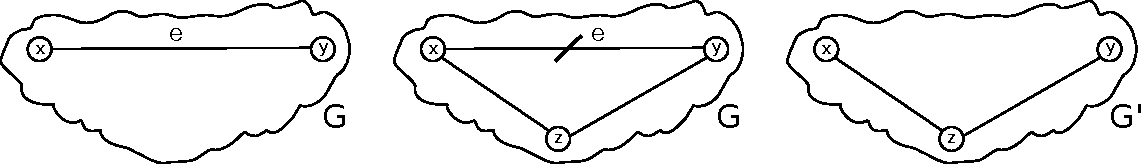
\includegraphics[scale=0.8]{images/n_09}
  \end{center}
Da $G$ costruiamo il grafo $G'$ ottenuto rimuovendo l'arco $(x, y)$ ed aggiungendo il nodo $z$ e due nuovi archi $(x, z)$ e $(y, z)$. Spostiamo sui due archi $(x, z)$ e $(y, z)$ le porte dell'arco $e$. Assumiamo che   $z$ non sia l'iniziatore del protocollo. Ripetiamo la \underline{stessa esecuzione} di $A$ su $G'$ (supponendo quindi che lo stesso ritardo di comunicazione avvenga, ovvero che quando x riceveva un messaggio su G lo riceve nello stesso momento anche su G') per fare in modo che sia sempre lo stesso arco in cui non transitino messaggi. \'E possibile eseguire la stessa identica esecuzione di A perchè nessun messaggio viene inviato sull'arco (x,y) (su G' nemmeno c'è questo arco).\\
Se cosi fosse in G' nello stato finale c'è un nodo, lo $z$, che non viene raggiunto dall'informazione $I$, poichè negli archi che abbiamo creato non viene spedito nessun messaggio. Ciò è assurdo e questo implica che $A$ non è un protocollo di broadcasting corretto.
  \begin{center}
    $M[$ \texttt{Broadcast, RI+} $] = \Omega(m)$
  \end{center}
  \fd
\end{proof}
}
\theorem{
  Il minimo numero di messaggi richiesti dal broadcasting sotto $RI+$ è $\Theta(m)$. \\ Il \texttt{Flooding} è \textbf{ottimo asintoticamente}.
}

\section{Broadcast su grafi particolari}
\subsection{Alberi}
Se $G$ è un albero, allora $m=n-1$.

\begin{center}
  $M[$ \texttt{Flooding, RI+} $] = 2m -n+1 = 2(n-1) -n+1 =  2n-2-n+1 = n-1 = O(n)$
\end{center}

Possiamo considerare il lower bound $\Omega(n)$: \texttt{Flooding} è ottimo.

\subsection{Grafi completi}
Se $G$ è un grafo completo, allora $m = \frac{n(n-1)}{2} = O(n^2)$.

\begin{center}
  $M[$ \texttt{Flooding, RI+} $] = 2m-n+1 = O(n^2)$

  $T[$ \texttt{Flooding, RI+} $] = d = O(1)$
\end{center}

Considerando il lower bound $\Omega(n)$ allora Flooding \textbf{non} è ottimo.

Nel caso in cui $G$ sia completo, possiamo progettare un algoritmo (\texttt{KBcast}) ottimo in cui l'initiator, semplicemente, manda un messaggio ai suoi vicini che sono $n-1$, ottenendo quindi i seguenti costi:
\begin{center}
  $M[$ \texttt{KBcast, RI+} $] = n-1$

  $T[$ \texttt{KBcast, RI+} $] = 1$
\end{center}

In pratica abbiamo messo a NIL questa istruzione: \texttt{idle x, receiving(I)}

\subsection{Ipercubi}
\begin{itemize}
    \item Un Ipercubo Orientato $H_1$ di dimensione $k=1$ è una coppia di nodi chiamati in binario 0 ed 1 connessi da un singolo arco la cui porta è 1 in entrambe le parti. Da notare che K è anche il valore nel pedice dell' H, quindi è sia i numeri di porta sia nel pedice.
    \item Un Ipercubo Orientato $H_k$ è ottenuto connettendo i due ipercubi di dimensione $k-1$ chiamati $H'_{k-1}$ e $H''_{k-1}$ e collegando i nodi con lo stesso nome con un link di etichetta $k$ in entrambi i nodi. Quando si va a creare un nuovo Hypercubo, si aggiunge uno 0 davanti alle etichette dell'hyperubo già presente e in quello nuovo creato si aggiunge un 1 davanti. 
\end{itemize}

\begin{itemize}
  \item $H_1$: Due nodi collegati tra di loro.
  \begin{center}
    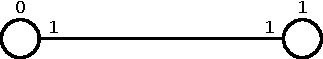
\includegraphics[scale=0.8]{images/n_10}
  \end{center}
  Come etichetta ai link si mette la dimensione dell'ipercubo.
  
  \item $H_2$
  \begin{center}
    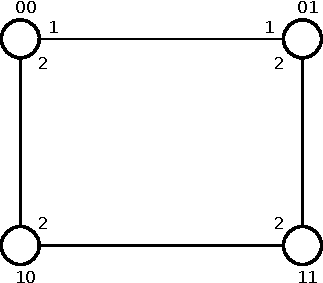
\includegraphics[scale=0.8]{images/n_11}
  \end{center}
  Due nodi adiacenti differiscono di uno ed un solo bit. Aggiungiamo un bit di prefisso ad ogni ``nome'' di nodo.
  Il valore $k$ è l'etichetta massima che si inserisce sugli archi. Per esempio se fossero presenti 8 nodi, ovvero il prossimo passo della figura sopra, il k sarebbe 3, poichè $k = \log_2{n}$; log in base 2 di 8 fa proprio 3.
\end{itemize}

Un ipercubo di dimensione $k$ ($H_k$) avrà:
\begin{itemize}
  \item $n = 2^k$ nodi, quindi $k = \log_2{n}$;
  \item $m = n \frac{k}{2} = \frac{n}{2} \log n$ Perchè ogni nodo ha $k$ collegamenti etichettati $1,2,..,k$. Dato che abbiamo archi in comune viene $\frac{n}{2}$
\end{itemize}

Quindi, il costo del \texttt{Flooding} è il seguente:

$M[$ \texttt{Flooding, RI+} $] = 2m-n+1 = \cancel{2}(\frac{n}{\cancel{2}} \log n)-n+1 = n(\log n -1) +1 = n(\log n -\log 2) +1 = n\log{\frac{n}{2}}+1 = O(n \log n)$

Possiamo vedere che il costo del \texttt{Flooding} su ipercubi non è $O(n)$ e quindi non siamo ottimi. Vediamo ora un miglioramento di tale algoritmo adatto a questo tipo di reti. 

\subsubsection{Protocollo Hyperflood}
Il funzionamento è il seguente:
\begin{enumerate}
  \item l'initiator manda il messaggio a tutti i suoi vicini;
  \item un nodo che riceve il messaggio da un link etichettato con $l$, manda il messaggio soltanto ai vicini con $l' < l$.
\end{enumerate}
L'unica differenza tra HyperFlood e il normale Flooding è nel passaggio 2: invece di inviare il messaggio a tutti i vicini tranne il mittente, l'entità lo inoltrerà solo ad alcuni di essi, che dipenderanno dall'etichetta della porta da cui il messaggio viene ricevuto.

\begin{lstlisting} [caption={\textit{Protocollo HyperFlood.}}]
S = {INIZIATORE, IDLE, DONE}
$S_{INIT}$ = {INIZIATORE, IDLE}
$S_{START}$ = {INIZIATORE}
$S_{TERM}$ = $S_{FINAL}$ ={DONE}
Restrictions = R

INIZIATORE
    Spontaneously
    begin
        send(m) to N(x)
        become DONE
    end

IDLE
    Receiving(M)
    begin
        LET $l$ be the port from where M arrived
        send(M) toward any $l'<l$
        become DONE 
    end
\end{lstlisting}

Vedremo che questa strategia effettuerà correttamente il broadcast usando solo $n-1$ messaggi (invece che $O(n \log n)$).
Sia $H_k(x)$ il sottografo di $H_k$ indotto dai link su cui vengono spediti messaggi del protocollo HyperFlood dove $x$ è l'iniziatore. Chiaramente ogni nodo in $H_K(x)$ riceverà l'informazione. Bisogna dimostrare che $H_k(x)$ tocca tutti i nodi: in questo modo, il protocollo \texttt{HyperFlood} è \textbf{corretto}.

\properties{
HyperFlood termina correttamente
\begin{proof}
%Dimostriamo che $\forall y \in \xi$ esiste un cammino da $x$, che consideriamo l'iniziatore, a $y$ in $H_k$ tale che la sequenza di etichette incontrate sia decrescente, ovvero 
Bisogna provare che se all'entità y arriva un messaggio dalla porta 4, l'entità lo invierà solo alle porte 1,2,3.
Per provare che ogni entità riceverà l'informazione inviata da $x$, dobbiamo mostrare che, per ogni nodo $y$, esiste un cammino da $x$ ad $y$ tale che la sequenza di porte attraversate durante il cammino è decrescente.
Per effettuare questa prova introduciamo la seguente proprietà:
\end{proof}
}
\properties{
  In un ipercubo $H_k$, $k$-dimensionale, ogni nodo $x$ è connesso ad ogni altro nodo $y$ da un cammino $\Pi \in [x,y]$ tale che la sequenza di etichette che si incontrano percorrendo $\Pi$ da $x$ ad $y$ è decrescente.
\begin{proof}
  Consideriamo i due nodi $x,y$ dell'ipercubo $H_k$ e siano:
  \begin{center}
    $<x_k, x_{k-1}, \ldots, x_1,x_0>$
    $<y_k, y_{k-1}, \ldots, y_1,y_0>$
  \end{center}
  le etichette binarie di $x$ ed $y$.

  Se $x$ e $y$ sono due nodi diversi allora il numero di bit su cui le due stringhe differiscono sarà:
  \begin{center}
    $t \geq 1$
  \end{center}

  Siano $j_1, j_2, \ldots, j_t$ tali posizioni in ordine decrescente, ovvero che $j_i > j_{i+1}$, consideriamo la sequenza di nodi:
  \begin{center}
    $v_0, v_1, \ldots ,v_t$
  \end{center}
  dove $v_0 = x$ e l'etichetta binaria del nodo $v_i$ differisce da quella di $v_{i+1}$ solo nella $j_{i+1}$ posizione.
  \begin{center}
    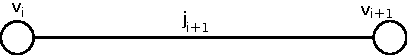
\includegraphics[scale=1]{images/n_12}
  \end{center}
  
  Se adesso prendo i nodi $v_0 = x $ e $v_1$, per costruzione saranno connessi dall'arco con etichetta $j_1$. Ma ancora per costruzione, $v_1$ sarà collegato a $v_2$ con l'etichetta $j_2$ e così via. Questa sequenza di nodi fa si che $v_t =  y$, ma questo significa che $<v_0, v_1, \ldots ,v_t>$\ è un cammino tra x ed y e la sequenza di etichette in questo cammino $<j_1, ..., j_t>$ è decrescente. Quindi $H_k(x)$ è connesso e contiene tutti i nodi di $H_k$ indipendentemente da $x$.\\
  In altre parole, entro un tempo finito, ogni entità avrà le informazioni.

\end{proof}
}

\textbf{Costo:}
\begin{center}
    $M[$\texttt{HyperFlood}$ / H_k] = n - 1$\\
    %$T[$\texttt{HyperFlood}$ / H_k] = k = \log (n) $
\end{center}
\textbf{Dimostrazione del Bound per i messaggi:}
Per provare che solo $n-1$ messaggi vengano inviati durante il broadcast \textbf{bisogna mostrare che ogni entità riceverà l'informazione solamente una volta.} Questo è vero perchè, per ogni entità $x$, $H_k(x)$ non contiene cicli se si utilizza il protocollo HyperFlood.\\
Per avere $M[$\texttt{HyperFlood}$ / H_k] = n -1$ dobbiamo dimostrare che $H_k(x)$ è un albero, ovvero che non ci sono cicli
\begin{proof}
Per induzione sulla dimensione $k$\\
\textbf{Base [$k=1$]: }$H_1(x)$ non ha cicli, poiché sono solo 2 nodi connessi fra di loro \\
\textbf{Induzione: } Supponiamo vero per $H_{k-1}(x)$ e supponiamo vero anche per $H_k(x)$ \\
Supponiamo quindi che $x$ sia l'iniziatore del protocollo, per come lo abbiamo definito, invierà un messaggio a tutti i suoi vicini $1, 2, ..., k$.
\begin{itemize}
    \item In $H_{k-1}(x)$ ha lo stesso comportamento di un ipercubo di dimensione $k-1$, ma questo per induzione non conteneva cicli.
    \item Sia $y$ l'entità che è dall'altra parte dell'arco con etichetta $k$, il discorso vale anche per lei, per induzione.
    \item  $H_{k}(x)$ è formato da due grafi aciclici connessi da un singolo arco, che quindi è a sua volta aciclico.
\end{itemize}

Costruiamo $H_k(x)$ e rimuoviamo l'arco k-esimo dall'iniziatore, avremo quindi due $H_{k-1}(x)$ separati, per che ipotesi induttiva non avevano cicli.\\
Ma allora neanche $H_k(x)$ può averne poiché per crearlo ho aggiunto un unico arco per unire due alberi.
\end{proof}

\textbf{Costo del Tempo:}\\
Il diametro di un Hypercubo è proprio $k$, infatti per qualunque coppia di nodi esiste sempre un cammino con etichette decrescenti tra i due nodi, e la lunghezza di questa commino è al più $k$.
\begin{center}
    $T[$\texttt{HyperFlood}$ / H_k] = k = \log(n) $
\end{center}
$k=\log(n)$ perchè abbiamo dimostrato che $H_k(x)$ è un albero.


\properties{
  Il tempo ideale necessario per il broadcasting su ipercubi $k$-dimensionali sotto RI+ è $\Theta(k)$.
}

Poiché $\Omega$ del broadcasting è il diametro che in un ipercubo è $k$.

\properties{
  Il numero di messaggi necessari per il broadcasting su ipercubi $k$-dimensionali sotto RI+ è $\Theta(n)$.
}


\chapter{Wake-Up}
Molto spesso, in un ambiente distribuito, ci troviamo di fronte alla seguente situazione:\\
Deve essere svolto un compito in cui devono essere coinvolte tutte le entità; tuttavia solo alcune di esse sono indipendentemente \textbf{attive} (a causa di un evento spontaneo, o per aver terminato un calcolo precedente) e pronte per il calcolo, le altre sono \textbf{inattive}, nemmeno consapevoli del calcolo che deve avvenire. \\
In queste situazioni, per eseguire il compito, dobbiamo assicurarci che tutte le entità diventino attive. Chiaramente, questo passaggio preliminare può essere avviato solo dalle entità già attive; tuttavia, non sanno quali altre entità (se presenti) sono già attive.\\
Questo problema è chiamato \textbf{Wake-up}: un'entità attiva è solitamente chiamata \textbf{awake}, un'entità inattiva (ancora) è chiamata \textbf{asleep}; il compito è svegliare tutte le entità.\\
Non è difficile vedere la relazione tra il broadcasting e il wake-up: \textbf{il Broadcasting è un wake-up con una sola entità inizialmente sveglia; al contrario, il wake-up è un broadcasting con possibilmente molti iniziatori} (cioè, inizialmente più di un'entità ha le informazioni). In altre parole, \textbf{il broadcasting è solo un caso speciale del problema del wake-up}.\\
È interessante, ma non sorprendente, che la strategia di flooding utilizzata per il broadcasting risolva effettivamente il problema più generale del wake-up. Il protocollo modificato è chiamato WFlood. Inizialmente tutte le entità sono \textit{asleep}; qualsiasi entità \textit{asleep} può svegliarsi (diventare \textit{awake}) spontaneamente e avviare il protocollo.\\
Non è difficile verificare che il protocollo termini correttamente con le restrizioni standard. \vspace{1cm}\\

\section{Protocollo WFlood}
\textbf{Problema}: Il problema del wake-up consiste nell'avere una configurazione iniziale del nostro sistema in cui possono essere presenti più entità sveglie (in stato di AWAKE) al tempo $t=0$ (ovvero più iniziatori) e le restanti entità saranno dormienti (ASLEEP). Al termine del protocollo vogliamo che tutte le entità siano sveglie (AWAKE). Utilizzeremo sempre l'idea del Flooding, ovvero un'entità invia l'informazione a tutti i suoi vicini tranne quello che gliel'ha inviata. Formalmente:

$P_{INIT} =<\; \forall x \in \xi, STATUS(x) = ASLEEP \;>$\\
$P_{FINAL} =<\; \forall x \in \xi, STATUS(x) = AWAKE \;>$\\

\begin{lstlisting} [caption={\textit{Protocollo WFlood.}}]
S = {AWAKE, ASLEEP}
$S_{INIT} = S_{START}$ = {ASLEEP}
$S_{TERM}$ = $S_{FINAL}$ ={AWAKE}
Restrictions = R

ASLEEP
    Spontaneously
    begin
        send(W) to N(x)
        become AWAKE
    end
    
    Receiving(W)
    begin
        become AWAKE
        send(W) to N(x) - sender
    end
\end{lstlisting}

\textbf{Descrizione del protocollo (codice)}: $P_{init}$ ci dice che tutte le entità all'inizio si trovano sullo stesso stato, che è quello di Asleep. Successivamente verranno svegliate (e quindi cambieranno stato) in base agli impulsi spontanei che ricevono e quello sarà il numero degli iniziatori. Quando ricevono questo impulso spontaneo inviano l'informazione a tutti i vicini e cambiano stato in "AWAKE". Quando un'entità nello stato di ASLEEP riceve il messaggio allora diventa AWAKE e lo invia a tutti i suoi vicini meno il sender. In poche parole, solamente gli iniziatori lo inviano a tutti, i restanti lo inviano a tutti meno il sender.

\subsection{Complessità del problema}
\underline{Messaggi:}
Il numero di messaggi è almeno pari a quello del broadcast; in realtà, non è molto di più.
\begin{center}
  Caso Migliore $(\Omega)$: $M[$\texttt{WFlood}$] \geq 2m - n + 1$  \\
\end{center}
E questo avviene quando c'è un solo iniziatore come nel Broadcast e quindi tutte le entità meno una riescono a risparmiare messaggi.\\
\begin{center}
Caso Peggiore $(O)$: $M[$\texttt{WFlood}$] \leq 2m$\\ 
Caso generico con $k^*$ iniziatori: $2m-n+1 + k^* -1 = 2m-n+k^*$ 
Dove il -1 è l'iniziatore già incluso in 2m-n+1

$M[$\texttt{Wake-Up}$/R] \geq M[$\texttt{Broadcast}$/RI+] = \Omega(m)$\\
  \texttt{WFlood} è ottimo per i messaggi.
\end{center}
Il caso peggiore accade quando tutte le entità si svegliano con l'impulso spontaneo ($n$ initiator).

\subsubsection{Dimostrazione del Lower Bound pari ad m}
Sia A un algoritmo che permette di risolvere il problema del Wake-up con un numero di messaggi minori di M. Questo significa che se applicassimo A su un generico grafo G allora ci sarebbe almeno un arco nel quale non vengono scambiati messaggi. Supponiamo che sia proprio l'arco tra $x$ ed $y$ denominato $e$. Andiamo adesso a costruire un nuovo grafo, chiamato $G'$ ottenuto rimuovendo l'arco $e$ tra x ed y e spostando le sue porte tra i nodi $x$ e $z$ e $y$ e $z$. A per essere un algoritmo che risolve il problema in oggetto deve dare soluzione su tutte le esecuzioni ed indipendentemente dalla configurazione iniziale. Vogliamo quindi dimostrare che esiste almeno un esecuzione di A tale per cui l'algoritmo fallisce. Andiamo quindi ad applicare la stessa identica esecuzione del protocollo A che aveva su G in G' ovvero:
\begin{itemize}
    \item Tutti gli iniziatori che abbiamo avuto su G li ritroviamo su G', su G $z$ nemmeno era presente quindi non può essere iniziatore.
    \item Tutti i tempi ed i ritardi di comunicazione che abbiamo osservato su G li riportiamo su G', ovvero che se un messaggio inviato ad un generico nodo ci metteva 30 secondi ad arrivare in G allora ci mette 30 secondi anche su G'.
    \item Possiamo eseguire la stessa esecuzione di A perchè in G l'arco in cui non transitavano messaggi è proprio $e$ ed in G' $e$ nemmeno è presente quindi sicuramente non verranno scambiati messaggi su quell'arco
    \item in poche parole forziamo la stessa identica esecuzione su G'.
\end{itemize}
Dato che in quella specifica esecuzione $x$ ed $y$ non inviavano messaggi sulle porta dell'arco $e$, in questo caso non invieranno i messaggi al nodo $z$. Quindi quando il protocollo termina tutti i nodi avranno raggiunto uno stato terminale, tranne $z$ che è ancora in stato di Asleep. Abbiamo quindi individuato un esecuzione in cui l'algoritmo A fallisce. Se fallisce per UN esecuzione non possiamo dire che l'algoritmo da soluzione al problema, e quindi si contraddice l'ipotesi.\\

Il tempo ideale sarà, in generale, più piccolo di quello per il broadcasting:\\
\underline{Tempo:}
\begin{center}
 T[$\texttt{Broadcast}/RI+] \geq T[\texttt{Wake-Up}/R] = \Omega(d)$\\
  $T[\texttt{WFlood}] = \Theta(d)$\\
\end{center}
\texttt{WFlood} è ottimo per il tempo (con più initiator si fa prima).\\

Tuttavia, nel caso di un unico iniziatore, i due casi coincidono. Poiché i limiti superiore e inferiore coincidono in ordine di grandezza, possiamo concludere che il protocollo WFlood è ottimale sia per numero di messaggi che in termini di tempo.\\
La complessità di Wake-Up è riassunta dalle seguenti due proprietà,
\begin{itemize}
    \item \textbf{La complessità dei messaggi del Wake-up sotto R è $\Theta(m)$}
    \item \textbf{La complessità del tempo del Wake-up sotto R è $\Theta(d)$}\\
\end{itemize}

\section{WFlood su grafi particolari}
\subsection{Alberi}
Il costo dell'utilizzo del protocollo WFlood per il wake-up dipenderà dal numero di iniziatori. Infatti, se c'è un solo iniziatore, allora questo è solo un broadcast e costa solo $n - 1$ messaggi ($m=n-1$). Al contrario, se ogni entità inizia indipendentemente, ci saranno un totale di $2(n - 1)$ messaggi. Quindi:
  \begin{center}
    Caso peggiore:$M[$\texttt{WFlood}$/R] \leq 2(n-1)$ \\
    (tutti sono iniziatori quindi essendo $m = n-1$ abbiamo $2 n-2$)
  \end{center}
  Supponiamo di avere $k^*$ iniziatori con $k^* \leq n$:
  \begin{center}
     $M[$\texttt{WFlood}$/R;T]= 2(n-1) - (n-k^*) = n+k^*-2$\\
    \begin{itemize}
        \item $2(n-1)$ è il caso peggiore a cui vanno tolti:
        \item $(n-k^*)$ Tutte le entità non iniziatrici.
    \end{itemize}
  \end{center}
    
\subsection{Ipercubi}
Nelle precedenti sezioni abbiamo trovato un modo per far scendere il costo del Broadcast su ipercubi da $O(nlogn)$ a $O(n)$. Nel caso del Wake-up però non è possibile abbassare il costo, poichè essendoci più iniziatori non vale la regola del mandare il messaggio a tutte le etichette minori di quella in cui un'entità ha ricevuto un messaggio. Quindi:
\begin{center}
  $M[$\texttt{Wake-Up}$/R;H_k] = \Omega(n \log n)$ \\
\end{center}
Deve transitare almeno un messaggio per arco, ed essendo il costo anche $O(n \log n)$ siamo ottimi.\\
%Diversamente dal problema del \texttt{Broadcast}, qui non possiamo utilizzare l'\texttt{HyperFlood} in quanto possiamo avere più initiator.\\
Il tempo quindi rimane lo stesso.
\begin{center}
     $T[$\texttt{WFlood}$/R;H_k] \leq d = k = \log n$ \\
\end{center}
Dove $k$ è l'eccentricità di un nodo all'interno dell'hypercubo
    
\subsection{Grafi completi}
Tramite l'utilizzo del generico protocollo WFlood il costo sarà il seguente:
\begin{center}
  Caso Peggiore: $M[$\texttt{WFlood}$/R] = O(m) = O(n^2)$ \\
  Caso Migliore: $M[$\texttt{Wake-Up}$/R;k] = \Omega(n^2)$
\end{center}
Utilizzando il protocollo del KBcast e se si svegliassero $k^*$ entità il costo sarebbe $k^*(n-1)$, ma nel caso peggiore $k^*$ è proprio $n$ quindi il caso peggiore sarebbe comunque O($n^2$). 
\begin{center}
  $M[$\texttt{KBcast}$/R] = k^*(n-1) = O(n^2)$
\end{center}
Questo perchè ogni $k^*$ iniziatore invia un messaggio a tutto il suo vicinato che è $n-1$. Però $1\leq K^* \leq n$ quindi il bound resta comunque O($n^2)$

Quindi con il \texttt{WFlood} siamo ottimi, anche se il costo è alto e non è possibile usare il \texttt{KBcast} visto nel problema del \texttt{Broadcast} su grafi completi in quanto non si ottengono migliorie di nessun tipo.

\subsection{Grafi completi con identificatori}
Dato che non si riesce a diminuire il costo del protocollo tramite l'utilizzo del KBcast, andiamo ad aumentare il numero di restrizioni all'insieme R. Aggiungiamo quindi la restrizione \textbf{Restriction Initial Distinct Values (ID)}: ogni nodo adesso ha associato un identificatore unico che lo distingue dagli altri.
In questo caso possiamo creare un protocollo, che chiameremo \texttt{WFlood+} con il seguente costo:
%\begin{center}
%  $M[$\texttt{WFlood+}$/R;K_n;id] = O(n \log n)$
%\end{center}


\theorem{$M[$\texttt{WFlood+}$/R;K;ID] \geq 0.5n \log n$}\\
%\textbf{Lemma:} Il numero di messaggi nel problema del WAKE-UP sotto le restrizioni di grafo completo e identificatore unico è $\frac{1}{2} n \log n$
Possiamo dimostrare che siamo ottimi, ovvero che siamo anche $O(n \log n)$ tramite la tecnica dell'avversario.

\subsubsection{Tecnica dell'avversario}
Per costruire il peggior scenario possibile per un protocollo A di Wake-up, consideriamo un gioco tra le entità ed un avversario. Le entità devono obbedire alle regole del protocollo, mentre l'avversario cercherà di creare lo scenario peggiore possibile, forzando le entità ad inviare il maggior numero di messaggi.

\textbf{Assunzioni:} assumiamo che $n$ sia una potenza di due: $n = 2^p$, ovvero che le entità che si svegliano sono una potenza di due.

\textbf{Poteri dell'avversario: [SIAMO SU GRAFO COMPLETO]}
\begin{enumerate}
  \item Decide i valori iniziali delle entità (id), purché siano tutti distinti;
  \item Decide quale entità spontaneamente inizia l'esecuzione di A e quando;
  \item Decide quando un messaggio spedito arriva (in tempo comunque finito);
  \item Decide il matching tra gli archi e le etichette (porte). Durante l'esecuzione, quando $x$ effettua l'operazione "Invia messaggio alla porta $l$" ed $l$ non è stata ancora assegnata, l'avversario sceglierà su quale collegamento non ancora utilizzato (ovvero che non sono stati ancora inviati messaggi) assegnare porta $l$.
\end{enumerate}

L'invio di un messaggio a più di una porta verrà trattato come l'invio del messaggio a ciascuna di tali porte una alla volta (in un ordine arbitrario).\\
Qualunque cosa decida l'avversario, può accadere in una vera esecuzione. Vediamo quanto male può creare un caso l'avversario per A.\\
Due insiemi di entità si diranno \textbf{connessi all'istante $t$} se almeno un messaggio è stato trasmesso da un'entità di un insieme a un'entità dell'altro.

\textbf{Sviluppo del peggior scenario possibile:}
\begin{enumerate}
    \item Inizialmente l'avversario sveglia una sola entità s, che chiameremo Seed, che inizierà l'esecuzione del protocollo. Quando s decide di inviare un messaggio ad una certa porta l, l'avversario sveglierà un'altra entità $y$ e assegnerà porta l all'arco tra s e y. Successivamente ritarda la trasmissione del messaggio fin quando $y$ non decide di inviare un messaggio ad un'altra porta $l'$; l'avversario assegnerà porta $l'$ al collegamento tra $y$ ed $s$ e farà in modo che i due messaggi inviati arrivino contemporaneamente. In questo modo ogni messaggio raggiungerà un nodo già sveglio e le due entità saranno connesse.\\
    D'ora in poi, l'avversario agirà in modo simile; assicurarsi sempre che i messaggi vengano inviati ai nodi già attivi e che l'insieme di nodi attivi sia connesso.
    \item Si consideri un'entità $x$ che esegue un'operazione di \textbf{invio} a un'etichetta non assegnata $a$.
    \begin{enumerate}
        \item Se $x$ ha un collegamento inutilizzato (cioè un collegamento su cui finora non sono stati inviati messaggi) che lo collega a un nodo attivo, l'avversario assegnerà $a$ a quel collegamento.\\
        In altre parole, l'avversario cercherà sempre di fare in modo che le entità sveglie inviino messaggi ad altre entità sveglie.
        \item Se sono stati utilizzati tutti i collegamenti tra $x$ e i nodi svegli, l'avversario creerà un altro insieme di nodi svegli e collegherà i due insiemi. 
        \begin{enumerate}
            \item Siano $x_0 , . . . , x_{k-1}$ i nodi attualmente attivi, ordinati in base al loro tempo di risveglio (quindi, $x_0 = s$ è il seed e $x_1 = y$). L'avversario eseguirà la seguente funzione: scegliere $k$ nodi inattivi $z_0 , . . . , z_{k-1}$ ; stabilire una corrispondenza logica tra $x_j e z_j$ ; assegnare i valori iniziali alle nuove entità in modo che l'ordine tra esse sia uguale a quello tra i valori delle entità corrispondenti; svegliare queste entità e costringerle ad avere la "\textbf{stessa}" esecuzione (stessa programmazione e stessi ritardi) come già avevano le corrispondenti. (Quindi, $z_0$ verrà svegliato per primo, il suo primo messaggio verrà inviato a $z_1$ , che verrà svegliato successivamente e invierà un messaggio a $z_0$ , e così via)
            \item L'avversario assegnerà quindi l'etichetta $a$ al collegamento che collega $x$ alla sua corrispondente entità $z$ nel nuovo set; il messaggio verrà tenuto in transito fino a quando $z$ (come ha fatto $x$) dovrà trasmettere un messaggio su un collegamento inutilizzato (diciamo, con etichetta $b$) ma tutti i bordi che lo collegano al suo insieme di entità sveglie sono già stati utilizzati.
            \item Quando ciò accade, l'avversario assegnerà l'etichetta $b$ al collegamento da $z$ a $x$ e farà arrivare ed elaborare i due messaggi tra $x$ e $z$.
        \end{enumerate}
        In altre parole, questo punto può essere descritto come segue:\\
        Se tutti i link tra un'entità $x$ ed un altro nodo sveglio sono tutti stati utilizzati ed $x$ vuole inviare un messaggio ad una nuova porta, allora l'avversario creerà un altro set di nodi (già svegli) e li forzerà ad avere la stessa esecuzione del set su cui si è basato. Dato che eseguono la stessa esecuzione, quando l'entità vorrà inviare un messaggio ad una certa porta che conduce ad entità NON sveglie, allora l'avversario assegnerà la porta nel link che conduce all'entità che inizialmente voleva inviare un messaggio nell'altro set e farà in modo che i due messaggi arrivino contemporaneamente. \\\textbf{[Quindi ci si basa sulla "stessa esecuzione"]}\\
        Successivamente ripeterà sempre le stesse esecuzioni, ovvero farà in modo che entità sveglie invino messaggi ad altre entità sveglie fin quando può.
    \end{enumerate}
\end{enumerate}
\textbf{Riassunto:} L'avversario cercherà di forzare il protocollo per far si che si invino messaggi sempre ad entità già sveglie e consegnerà i messaggi solamente quando non può fare altrimenti. Il numero delle entità che l'avversario sveglia è uguale al numero di quelle già sveglie e queste saranno forzate ad avere la stessa esecuzione di quelle già sveglie. Quando tutti i collegamenti sono terminati l'avversario inizia un nuovo Stage.

\subsubsection{Analisi del costo}
  Siano:
  \begin{itemize}
      \item $Active(i)$ le entità sveglie allo stage $i$.
      \item $New(i) = Active(i) - Active(i-1)$  entità che l'avversario sveglia nello stage $i$. Queste sono in numero uguale a quelle già sveglie, quindi: $|New(i)|=|Active(i-1)|$ 
      \item $Seed = Active(0)$ ovvero la prima entità che l'avversario sveglia.
      \item $\mu(i-1)$ il numero totale di messaggi inviati prima dell'attivazione delle nuove entità.% allo stage $i-1$ %dell'attivazione delle nuove entità.
  \end{itemize}
   Una volta che la connessione avviene, quanti messaggi vengono trasmessi prima del nuovo stage?\\
  Dato che colleghiamo due set, il numero di messaggi scambiati prima della connessione sarà esattamente $2\mu(i-1)$. Quindi a questo punto abbiamo:
   $$\mu(i) \geq 2\mu(i-1) + Qualcosa$$
   Dove quel qualcosa sono tutti i messaggi che vengono inviati dall'avversario per fare in modo che entità sveglie inviino messaggi ad altre entità già sveglie (sono tutti i messaggi che l'avversario fa sprecare). A questo punto abbiamo:
 
 %Supponiamo che $A$ sia il miglior algoritmo possibile per risolvere il problema, ovvero che fa in modo che sia solamente una singola entità ad inviare messaggi ogni volta ad una porta diversa. Se così fosse l'avversario sarebbe costretto a svegliare una per una tutte le entità ed assegnare i numeri di porta per mandare i messaggi nella corretta direzione, quindi l'avversario dovrà inviare un messaggio ad ogni nuova entità . A questo punto abbiamo:
  $$\mu(i) \geq 2\mu(i-1) + |new(i)|$$
Questo è un Bound, non è detto che un algoritmo così esista, ma è la cosa migliore che possiamo aspettarci. Dato che però $|new(i)|=|active(i-1)|$ ed il numero di entità raddoppia ad ogni stage, abbiamo che:
\begin{itemize}
    \item $|Active(0)| = 1$
    \item $|Active(1)| = 2$
    \item $|Active(2)| = 4$
    \item ecc ecc
\end{itemize}
Abbiamo che \\
- $|active(i-1)| = 2^{i-1}$ Quindi in questo caso otteniamo:
 $$\mu(i) \geq 2\mu(i-1)+2^{i-1}$$
 Proviamo a svolgere adesso $\mu(i-1)$:
 $$\mu(i) \geq 2\mu(i-1)+2^{i-1} \geq 2(2\mu(i-2))+2^{i-2})+2^{i-1}$$
 Ma si arriverà ad un punto nel quale si avrà $i-i$ quindi questo si può maggiorare con:
  $$\mu(i) \geq i2^{i-1}$$
  Essendo che abbiamo scelto una potenza di $n=2^p$ Allora il numero totale di stage è esattamente $\log n$
  $$i \cdot 2^{i-1} = \log n \cdot 2^{\log n-1} = {\frac{1}{2}} n \log n$$
 
\textbf{Analisi del costo presa dal Libro:}\\
%\textbf{Ovvero: }Abbiamo collegato due set, quanti messaggi vengono scambiati in questo caso prima che questo set venga collegato con un altro? (cioè inizi un nuovo stage?)\\
Il numero esatto dipenderà dal protocollo A, ma indipendentemente da questo, l'avversario non inizierà lo stage $i+1$ fin quando non sarà forzato a farlo, ovvero quando un'entità $x$ che esegue un comando di "Invia a porta l" (dove $l$ è una porta che non è già stata utilizzata) non ha più vicini disponibili a cui inviare un messaggio. Questo significa che $x$ deve aver ricevuto o inviato messaggi da tutte le altre entità sveglie allo stage(i), ovvero quelle in $Active(i) = Active(i-1) \cup New (i)$.
 
 \begin{itemize}
     \item Assumiamo che $x \in Active(i-1)$, allora tra tutti questi i messaggi, quelli tra $x$ e $New(i)$ sono stati inviati allo stage(i), dato che queste entità non erano sveglie prima. Questo significa che almeno $|New(i)|=|active(i-1)|$ messaggi sono stati inviati prima dello stage $i+1$.
     \item Se invece $x \in New(i)$ (quindi $x$ non era sveglia fino ad adesso), questi messaggi saranno trasmessi tutti in questo stage. Anche in questo caso $|New(i)|=|active(i-1)|$ messaggi sono stati inviati prima dello stage $i+1$.
 \end{itemize} 
 
 Quindi, il costo totale $\mu(i-1)$ prima dello stage(i) è raddoppiato ed almeno $|active(i-1)|$ messaggi sono stati inviati prima dello stage (i+1). In simboli:

 %Il numero di messaggi inviati allo $stage(i)$ è sicuramente maggiore uguale a due volte il numero di messaggi scambiati allo stage precedente più il numero delle entità che l'avversario sveglia nello $stage(i)$. Quindi abbiamo:
 
 $$\mu(i) \geq 2\mu(i-1) + |Active(i-1)|$$
 
 Dato che il numero delle entità sveglie raddoppia ad ogni stage: $|Active(i-1)| = 2^{i-1}$ ed osservando che $\mu(0) = 0$ e che inizialmente solamente il seed è attivo, si ha:
 
 $$\mu(i) \geq 2\mu(i-1)+2^{i-1} \geq i2^{i-1}$$
 
 Il numero totale di stage $i$ è esattamente $log(n)$ poichè il numero delle entità sveglie raddoppia ad ogni stage. Quindi, con questa strategia, l'avversario può forzare qualsiasi protocollo a trasmettere almeno $\mu(\log n)$ messaggi. Sostituendo otteniamo che:
 
 $$i \cdot 2^{i-1} = \log n \cdot 2^{\log n-1} = {\frac{1}{2}} n \log n$$
 
 Ne segue quindi che ogni protocollo di wake-up trasmette $\omega(n \log n)$ messaggi nel peggiore dei casi, anche se le entità hanno id distinti. : $M[$\texttt{Wake-Up}$/R;k;id] = \Omega(n \log n)$

%DA QUI IN POI è VECCHIO\\
\begin{comment}
\begin{itemize}
  \item All'inizio tutte le entità sono dormienti (\texttt{ASLEEP}).
  \item L'avversario sceglie un'entità arbitraria la quale deve spedire messaggi.
  \begin{center}
    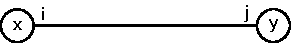
\includegraphics[scale=1]{images/n_14}\\
    (x e y diventano connessi)
  \end{center}
  \item Siccome l'avversario gioca contro le entità, prima di consegnare il messaggio di $x$, sveglia $y$ ed aspetta a consegnare il messaggio.
\end{itemize}
  In generale, quando $x \in  \xi$ vuole mandare un messaggio, l'avversario guarda i link a cui $x$ manda i messaggi e sveglia tutte le entità non ancora sveglie (posticipando la consegna dei messaggi).

  Supponiamo $G'$ sia il grafo composto da nodi svegli, consideriamo $G''$ composto da nodi non svegli isomorfo a $G'$:

  \begin{center}
    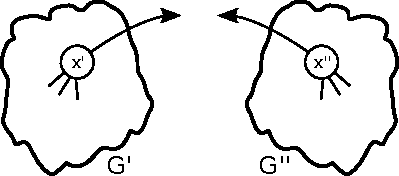
\includegraphics[scale=1]{images/n_15}
  \end{center}

  $G'$ e $G''$ sono sconnessi e sono isomorfi poiché consideriamo grafi completi.

  Quando creiamo il collegamento tra $G'$ e $G''$ diciamo che l'avversario è in un \textit{nuovo STAGE}.\\
 Quindi \textbf{STAGE(i)} equivale al momento in cui due sottoinsiemi di entità vengano unite dallo scambio reciproco di un messaggio.\\
\end{comment}


\chapter{Attraversamento}

\textbf{Problema}: Il problema dell'attraversamento consiste nell'avere una configurazione iniziale dove tutte le entità sono nello stesso stato (IDLE) eccetto una che sarà l'unico iniziatore. L'obiettivo è quello di visitare una alla volta tutte le entità in maniera sequenziale. Il messaggio che dovrà transitare tra le entità si chiama TOKEN (T).\\
\textbf{Formalmente:}\\
$
P_{INIT} = <\exists ! x \in \xi | Value(x) = T \;>
$\\
\textsc{Ovvero:} Esiste una sola entità all'interno del sistema che possiede il Token T, tutte le altre saranno in stato di Idle.

$P_{FINAL} = <\exists t>0 | \forall x \in \xi \exists t' \leq t | value_{t'}(x) = T$ and $value_{t'}(y) \neq T, \forall y \neq x >$\\
\textit{Ovvero:} Esiste un tempo t maggiore di 0 tale per cui per ogni $t' \leq t$ c'è una sola entità che detiene il token e per ogni entità esiste un tempo $t'' \leq t$ nel quale X è proprio la detentrice del token e nessun altra lo possiede.

\textbf{Restrizioni:} R, UI (iniziatore unico che detiene il Token).

\textbf{Tipologie di messaggi inviati:}
\begin{itemize}
    \item T : Messaggio di Token
    \item Return: Inviato da un nodo per avvertire il padre che il sottografo è stato completamente esplorato.
    \item Back\_Edge : T viene inviato ad un nodo che è già stato visitato, quell'arco viene catalogato come Back\_edge e da li non passeranno mai più token.
\end{itemize}
\textbf{Stati possibili dell'algoritmo:}
\begin{itemize}
    \item Idle
    \item Initiator
    \item Visited
    \item Done
\end{itemize}

\textbf{Caratteristica dell'algoritmo e differenza con il Broadcast:} Si effettua una visita sequenziale delle entità. Ovvero un'entità alla volta può possedere il Token T, quando un nodo riceve T, esso è marcato come "Visited".

\section{Funzionamento dell' algoritmo tramite DFS}
\begin{enumerate}
  \item Quando un'entità riceve per la prima volta il TOKEN, cambia stato in VISITED e crea l'insieme "Unvisited" che contiene tutti i suoi vicini tranne l'entità che gli ha spedito il token. Manda poi il TOKEN verso un nodo nell'insieme, lo rimuove da quest'ultimo e aspetta il messaggio di RETURN.
  \item Quando uno dei vicini riceve il TOKEN:
    \begin{itemize}
        \item Se è già stato visitato (VISITED), manda indietro un messaggio di BACK\_EDGE per poi rimuove il sender dal suo vicinato (così che non potrà inviargli T nemmeno per sbaglio).
        \item Altrimenti cambia stato in VISITED e spedisce il TOKEN sequenzialmente ad ogni suo vicino non visitato e successivamente manda il messaggio di RETURN verso il padre.
    \end{itemize} 
  \item Dopo la ricezione del RETURN, un'entità manda il TOKEN ad un altro vicino localmente non visitato.
  \item Se non ci sono più vicini disponibili, allora manda RETURN a sua volta.
\end{enumerate}

Quindi, l'insieme degli Unvisited viene aggiornato quando:
\begin{itemize}
    \item Un'entità manda il token
    \item Viene inviato un Backedge (ho sbagliato strada ma aggiorno comunque il mio insieme degli Unvisited per non sbagliare nuovamente).
\end{itemize}

\subsection{Protocollo DFTraversal}
\begin{lstlisting} [caption={\textit{Protocollo DFTraversal.}}]
S = {INITIATOR, VISITED, IDLE, DONE}
$S_{INIT}$ = {INITIATOR, IDLE}
$S_{START}$ = {INITIATOR}
$S_{TERM}$ = $S_{FINAL}$ = {DONE}
Restrictions = RI+

INITIATOR
    Spontaneously
    begin
        Unvisited := N(x)
        initiator := true // serve per terminare il protocollo
        VISIT
    end


Procedure VISIT
    begin
        if unvisited != 0 then
            next <- unvisited
            send(T) to next
            become VISITED
        else
            become DONE
            if not initiator then
                send(RETURN) to entry // a chi mi ha raggiunto la prima volta
    end

IDLE
    Receiving(T)
    begin
        unvisited := N(x) - sender
        entry := sender
        initiator := false
        VISIT
    end

VISITED
    Receiving(T)
    begin
        send(BACK_EDGE) to sender
        Unvisited := Unvisited - sender
    end
    
    Receiving(RETURN)
    begin
        VISIT
    end
    
    Receiving(BACK_EDGE)
    begin
        VISIT
    end
\end{lstlisting}
Notiamo che nell'insieme degli stati c'è anche \textbf{Done.} Un'entità 
entra in questo stato quando ha finito di esplorare il suo vicinato. Non è possibile quindi che gli venga inviato un token, poichè anche il suo vicinato sà che ha finito. I nodi Done quindi sono rimossi da tutti gli insiemi degli Unvisited.

\subsection{Costo dell'algoritmo}
Prendendo in esempio un singolo arco, le tipologie di messaggi che potranno transitare sono solamente due, il (TOKEN) e un (BACK\_EDGE o un RETURN).
Dato che il protocollo è sequenziale, si avrà che anche il Tempo è uguale al numero di Messaggi inviati.\\
\textbf{Costo dei Messaggi}
\begin{center}
  $M[$\texttt{DFT}$,R,UI] = 2m ~~$\\
  $M[DFTraversal] \geq m$
  \end{center}
  \textbf{Costo del Tempo:}
  \begin{center}
  $T[DFTraversal] = 2m$\\
     $T[$\texttt{DFT}$,R,UI] \geq n-1 $
  \end{center}
Dato che ogni nodo viene visitato sequenzialmente partendo dall'unico iniziatore, la complessità del tempo è almeno il numero di nodi, questo accade quando si invia il token sempre al nodo corretto. \underline{Non} è ottimo per il tempo. poichè si aveva un Upper Bound di O(m), che può essere di più ordini di grandezza maggiore del lower bound n-1. Possiamo trovare un esempio in un grafo completo, il cui costo salirebbe a $2m=n^2-n$.

\begin{center}
  $\mu(DFT/R) \geq m$
\end{center}
  Il numero di messaggi inviati è almeno $m$, è quindi $\Theta(m)$ per i messaggi e la dimostrazione è uguale a quella del broadcast.

\subsection{Avessimo utilizzato la BFS?}
Questo approccio risulta in un peggioramento sia su T che su M. Prendendo un nodo come esempio si avrebbe la seguente esecuzione:
Per ogni nodo si esplorano tutti i vicini (e quindi non il sottografo), poi si sceglie un vicino e si effettua la stessa cosa, e così via fin quando tutti i token che inviamo non ci tornano indietro come Backedge.

Questo risulta sicuramente in un costo peggiore della DFS, poichè i messaggi saranno sicuramente più di due per arco.

Tutto lo scambio dei messaggi avviene in modo sequenziale quindi per ridurre il tempo, o
\begin{itemize}
    \item Riduco il numero di messaggi.
    \item Li parallelizzo.
\end{itemize}

\section{DF+ miglioramento di DFTraversal}
La miglioria consiste nell' eliminare i messaggi di BACK\_EDGE. Al loro posto vengono introdotti i messaggi di VISITED e ACK. Quando un'entità riceve il TOKEN avvisa tutti i vicini (in parallelo) che è stato visitata (con messaggio di VISITED) ed aspetta da tutti un messaggio di ACK prima di spedire il token. Questo comporta che l'entità che spedisce il token sappia quale dei suoi vicini è già stato visitato e non potrà sbagliare. Viene aggiunto un nuovo stato, \textbf{"Avaiable"}; un'entità entra in questo stato quando, trovandosi nello stato di "Idle" riceve un messaggio di VISITED.\\

\textbf{A cosa servono nello specifico i messaggi di VISITED?}\\
Servono a far cambiare stato all'entità che lo riceve in AVAIABLE, ovvero che non ha ancora ricevuto il token. Se un'entità in stato AVAIABLE riceve un altro messaggio di VISITED allora elimina l'entità che glielo ha inviato da sul vicinato, poichè è sicura che quell'entità ha già ricevuto il token. Si può vedere dal codice del protocollo.\\
\textbf{Quindi, l'insieme degli Unvisited viene aggiornato quando:}
\begin{itemize}
    \item Un'entità manda il token
    \item Un'entità riceve un messaggio di VISITED. In questo caso cambia stato in Avaiable. In questo stato eliminerà tutti i suoi vicini dall'insieme degli Unvisited se questi gli mandano a loro volta messaggi di VISITED.
\end{itemize}

\textbf{Quanti messaggi per ogni tipologia vengono inviati?} 

\textbf{Innanzitutto i tipi di Messaggi inviati sono:} VISITED, ACK, T $(n-1)$, RETURN $(n-1)$

\begin{itemize}
  \item T e RETURN = Ogni entità eccetto l'iniziatore riceverà un singolo messaggio di T ed invierà un singolo messaggio di Return; l'iniziatore non riceverà nessun messaggio di T e non invierà nessun Return, quindi si hanno $2(n-1)$ messaggi di questo tipo.
    
  \item VISITED e ACK = Ogni entità eccetto l'iniziatore invia un messaggio di VISITED a tutti i suoi vicini eccetto quello che gli ha inviato il token; l'iniziatore invierà VISITED a tutti i vicini. Sia $s$ l'iniziatore, il numero di questi messaggi inviati è
  $$|N(s)| + \sum_{x \neq s} |N(x)| - 1 = 2m - (n - 1)$$
  Dato che ogni VISITED è seguito da un ACK:
  $2(2m - n + 1) = 4m -2n + 2$

\begin{center}
  $M[$\texttt{DF+}$/R] = 2(n-1) + 2(2m-n+1) = 4m$
\end{center}

  \textbf{Tempo} per Messaggi T e RETURN = $2(n-1)$ in quanto i messaggi sono sequenziali.
  
  \textbf{Tempo} per Messaggi VISITED ed ACK = $2n$ in quanto ogni nodo manda VISITED ai suoi vicini in una sola unità di tempo (parallelo) e tutti rispondono con un' ACK anch'esso parallelo, quindi il costo in tempo si incrementa di 2n. In questo caso i visited vengono inviati a tutti i vicini meno il sender, ma dato che vengono inviati in parallelo non conta QUANTI ne vengono mandati, basta sapere che ogni entità, per quanto riguarda il tempo, utilizza 1 singola unità per inviare Visited ed 1 singola unità per inviare ACK.
  
  \begin{center}
  $T[$\texttt{DF+}$/R] = 2(n-1) + 2n = 4n - 2 = O(n)$\\
\end{center}
\end{itemize}

Riassumendo, siamo riusciti a ridurre il costo del TEMPO da O(m) a O(n). Al prezzo di raddoppiare il numero di messaggi. 

\properties[2.3.2]{ La complessità ideale del tempo del DF+ sotto R è $\Theta(n)$}

\section{DF++ miglioramento di DF+}
Diminiuamo ancora il numero di messaggi, evitiamo di inviare messaggi di ACK. Se così fosse avremmo per esempio la seguente computazione:

\begin{center}
  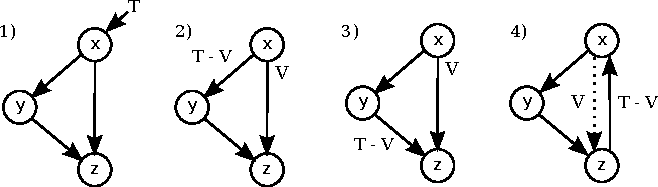
\includegraphics[scale=1.5]{images/n_17}
\end{center}

\begin{enumerate}
  \item $x$ riceve $T$ (TOKEN);
  \item $x$ invia il Token ad $y$ e un Visited ad $y$ e $z$ (supponiamo che il Visited verso $z$ abbia ritardi);
  \item $y$ riceve il Token, ed invia Token e Visited all'unico vicino disponibile, ossia $z$ (il Visited spedito da $x$ verso $z$ non è ancora arrivato);
  \item $z$ riceve il Token da $y$ e manda il Token e Visited verso $x$, dato che ancora non ha ricevuto il Visited da $x$. A questo punto $x$ riceve il Token da $z$ e capisce che $z$ ha commesso un errore, ignorerà quindi il Token ed elimina $z$ dalla lista dei suoi vicini. Nel momento in cui $z$ riceve il Visited di $x$, capisce che quello è un vecchio Visited (se $x$ era la prima volta che riceveva il Token, non avrebbe mandato un Visited a $z$), a questo punto $z$ capisce che ha inviato T al link sbagliato e quindi invia il Token ad un'altra strada (se disponibile), altrimenti manda RETURN verso $y$.
\end{enumerate}
Quindi il protocollo funziona anche senza i messaggi di "ACK", ma ammettiamo la possibilità di inviare T ad un nodo che lo ha già ricevuto, quindi la possibilità di sbagliare.\\
In questo caso $z$ se avesse ricevuto il VISITED da $x$ avrebbe cambiato stato in Avaiable ed avrebbe eliminato $x$ dal suo insieme degli Unvisited. A questo punto in ricezione del messaggio $T$ di $y$ avrebbe avuto l'insieme degli Unvisited Vuoto, e quindi avrebbe inviato un RETURN verso $y$.


\textbf{Andiamo ora ad analizzare il numero di messaggi utilizzati:}
\begin{itemize}
  \item \#$T$ e \#RETURN corretti = $2(n-1)$ 
  \begin{itemize}
      \item 2 è per i messaggi di T e RETURN
      \item $n-1$ indica tutti i nodi tranne l'iniziatore, poichè l'iniziatore non riceverà nessun messaggio di T e non invia nessun RETURN.
  \end{itemize}
  \item \#$T$ non corretti $\leq 2(m-n+1)$
  \begin{itemize}
      \item Ogni errore costa 1 messaggio, ma nel peggiore dei casi, il ritardo di comunicazione può forzare gli errori ad accadere in ogni arco che conduce al "sender" (back-edge), in alcuni ci possono essere anche due errori, uno in ogni direzione.
      
      
      %In ogni Arco $m$ posso sbagliare ma sicuramente non sbaglierò ad inviarlo al sender, quindi risparmio $-n+1$. Negli archi è possibile che si commettano due errori, uno in ogni direzione e da questo viene il 2.
  \end{itemize}
  
  \item \#VISITED = $2m - n + 1$, come nel \texttt{DF+}
  
\end{itemize}

\textbf{Andiamo infine a valutare i costi: }\\
\underline{Messaggi: (si sommano le tre quantità sopra)}
\begin{center}
  $M[$\texttt{DF++}$/R] \leq 4m - n + 1$
\end{center}

\underline{Tempo:}
Andiamo adesso ad effettuare una stima ideale del tempo, ovvero senza considerare gli errori che commetto. Al costo precedente di $4n-2$ devo togliere tutti i miglioramenti che applica questo protocollo:
\begin{center}
  $T[$\texttt{DF++}$/R] = 4n - 2 - n - n = 2n - 2$
\end{center}

Dove:
\begin{itemize}
  \item il primo $-n$ è degli ACK tolti;
  \item il secondo $-n$ è dei VISITED che posso inviare in parallelo con $T$ o con $RETURN$, nel caso in cui l'entità che riceve $T-V$ abbia l'insieme degli UNVISITED vuoto. Faccio questo perchè non devo aspettare niente di ritorno dalle entità in quanto gli ACK non ci sono più. 
\end{itemize}
Se non invio i Visited in parallelo allora il costo del tempo nel caso peggiore è $3n$.

\textbf{Nel caso in cui chieda direttamente questo protocollo:}
\begin{center}
  $T[$\texttt{DF++}$/R] = n-1 + n-1 = 2n - 2$
\end{center}
Dove:
\begin{itemize}
    \item $n-1$ sono i messaggi di T sia corretti che non. Non contiamo poi i Visited perchè vengono inviati in parallelo con T.
    \item $(n-1)$ sono i messaggi di Return
\end{itemize}

\section{DF*: Utilizzo di T come Visited Implicito}
Vediamo adesso un ulteriore miglioria applicabile al precedente protocollo: si possono utilizzare i messaggi di T come messaggi di VISITED impliciti, quindi nella direzione in cui invio T, non invio VISITED, ma in tutte le altre direzioni si.
Prima ad ogni invio di T si aveva un messaggio di VISITED sullo stesso link, questo non accade nella miglioria apportata. %si manda il messaggio di $T$ in parallelo con il messaggio di VISITED; quindi un $T$ corretto indica anche un VISITED.
\begin{center}
  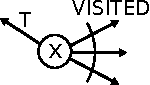
\includegraphics[scale=1]{images/n_19}
\end{center}
Il risparmio avverrà su tutte le entità \textbf{tranne} quelle che, quando vengono raggiunte per la prima volta da un messaggio T, hanno l'insieme degli UNVISITED già vuoto, ovvero che hanno già tutti i vicini già visitati dal Token e quindi non lo possono spedire a nessuno, \textbf{sono costrette ad inviare immediatamente return. Insieme a questo return l'entità invia ai suoi vicini meno quello a cui invia il RETURN i messaggi di visited, non risparmiando messaggi}. Sia $f^*$ questo numero di nodi, il numero di messaggi VISITED che salviamo è $n-f^*$ quindi:

\begin{center}
  $M[$\texttt{DF*}$/R] = 4m - n + 1 - (n - f^*)$
\end{center}

\begin{itemize}
    \item $ 4m - n + 1$: Il costo del protocollo $DF^{++}$ dove avevamo i T corretti, i T non corretti, i VISITED ed i RETURN.
    \item $n-f^*$ si ha un risparmio su tutti i nodi tranne esattamente $f^*$.
\end{itemize}
\begin{center}
  $T[$\texttt{DF*}$/R] = 2n - 2$
\end{center}
\begin{center}
  $M[$\texttt{DF*}$/R] = 4m - 2n + f^* + 1$
\end{center}
Al costo del protocollo precedente aggiungo un $-n+f^*$.
\begin{itemize}
  \item Caso migliore: grafo completo (ne risparmio $n-1$);
  \item Caso peggiore: stella (ne risparmio solo $1$).
\end{itemize}
Tra gli stati del protocollo c'è anche Avaiable.

Descrizione del protocollo a parole:
\begin{itemize}
    \item Iniziatore: Si sveglia tramite l'impulso spontaneo, crea l'insieme degli UNVISITED, composto da tutti i suoi vicini e ne sceglie uno (lo chiama "next"). Invia il token a questo e allo stesso tempo invia il  VISITED a tutto il suo vicinato meno quello a cui ha inviato il token.
    \item Idle: Se ricevo T allora creo l'insieme degli unvisited che contiene TUTTI i miei vicini (anche il sender), poi richiamo First-Visit.
    Se invece ricevo VISITED allora creo l'insieme degli unvisited che è composto da tutti i miei vicini meno il sender. Successivamente divento AVAIABLE.
    \item First-Visit: Elimino il sender dal mio insieme degli UNVISITED. Se quest'ultimo diventa vuoto, allora \textbf{invio RETURN al mio sender ed allo stesso tempo invio VISITED a tutto il mio vicinato meno il sender (a cui ho inviato return).} Poi divento DONE. Altrimenti scelgo un vicino dal mio insieme e gli invio il Token, mentre invio un VISITED a tutti i miei vicini tranne chi mi ha inviato il Token la prima volta e quello a cui ho inviato io il Token; successivamente divento VISITED. Altrimenti invio Return a mio "padre" ed allo stesso tempo invio il VISITED a tutti i miei vicini meno quello a cui ho inviato RETURN.
    \item AVAIABLE: Se ricevo T effettuo la first-visit. Altrimenti se ricevo VISITED aggiorno il mio insieme degli unvisited eliminando il vicino che mi ha inviato questo messaggio.
    \item VISITED: Se ricevo Visited allora aggiorno il mio insieme degli UNVISITED.
\end{itemize}


\section{Traversal in reti specifiche}
\subsection{Alberi}
In un albero la DFS è particolarmente efficente in termini di messaggi e non ha bisogno di nessuna miglioria. Infatti in un esecuzione del DF\_TRAVERSAL (il primo protocollo visto che aveva i messaggi di BackEdge) in un albero, nessun messaggio di BACKEDGE sarà inviato non essendo presenti cicli. Quindi il numero totale di messaggi è esattamente $2(n-1)$, stessa cosa per il tempo essendo sequenziale.
\begin{itemize}
  \item $m = n -1$
\end{itemize}
\begin{center}
  $T[$\texttt{DF}$/R] = 2(n-1) = O(n)$\\
  $M[$\texttt{DF}$/R] = 2(n-1) = O(n)$
\end{center}
%Essendo un albero aciclico, nessun messaggio di BACKEDGE verrà inviato, e non c'è bisogno di nessun miglioramento per il costo di entrambi.
\subsection{Anello}
In un anello, ogni nodo ha esattamente due vicini. La DFS in queste reti può essere applicata tramite la scelta di una direzione da parte dell'iniziatore, una volta che il messaggio di T ritorna indietro a lui il protocollo termina. Quindi ogni entità riceve un singolo messaggio di T; il costo sarà O(n).
\begin{itemize}
  \item $m = n$
\end{itemize}
\begin{center}
  $T[$\texttt{DF}$/R] = O(n)$
\\
  $M[$\texttt{DF}$/R] = O(n)$
\end{center}
Si può ottimizzare l'algoritmo scegliendo una direzione di invio.

\subsection{Grafi completi}
\begin{itemize}
  \item $m = O(n^2)$
\end{itemize}
L'esecuzione dell'algoritmo $DF^*$ richiederebbe O($n^2)$ messaggi. Un miglior protocollo potrebbe essere quello di fare in modo che l'initiator invii il token t sequenzialmente a tutti i suoi vicini uno alla volta; ogni entità ritorna poi il token all'initiator senza propagarlo a nessun altro. In questo caso il costo dei messaggi e del tempo sarebbe $2(n-1)$.
\begin{center}
  $T[$\texttt{DF}$/R] = 2(n-1)$\\
  $M[$\texttt{DF}$/R] = 2(n-1)$
\end{center}
Un'altra metodologia sarebbe quella di organizzare il grafo a stella:
\begin{center}
  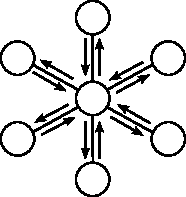
\includegraphics[scale=1]{images/n_20}
\end{center}
\begin{center}
      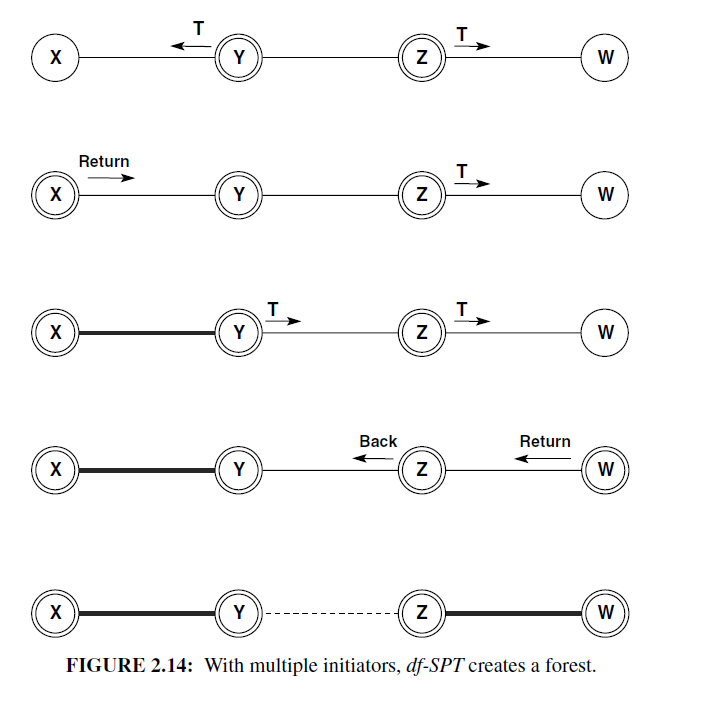
\includegraphics[scale=0.6]{images/asd.png}
    \end{center}


\chapter{Costruzione di uno Spanning Tree}
%Tutti i protocolli visti fino ad ora, hanno un numero di messaggi pari a $\Omega(m)$, dato che si lavora su grafi generici. Al crescere della rete, aumentano gli archi e quindi aumentano il numero di messaggi nei nostri protocolli. Questo va contro corrente all'idea di ampliare la rete per velocizzare il nostro sistema. L'idea è quindi quella di costruire uno Spanning Tree (Albero di copertura) e sfruttarlo poi in tutte le istanze dei nostri protocolli.
In un ambiente distribuito, costruire uno Spanning Tree di un grafo G significa muovere il sistema da una configurazione iniziale dove ogni entità è solo a conoscenza dei suoi vicini $N$, ad una configurazione dove:

\begin{enumerate}
  \item Ogni entità $x$ sceglie un sottoinsieme dei suoi vicini $N(x)$ come vicinato nello ST, chiamato TREE\_NEIGHBORS(x);
  \item L'insieme dei link corrispondenti forma uno ST di G.
\end{enumerate}
Quello che si vuole quindi è un algoritmo che, una volta eseguito, garantisce la costruzione di uno Spanning Tree $T(G)$ del grafo $G$.\\
\textbf{Le restrizioni} su cui faremo riferimento saranno $R+UI$.\\
Si noti che T non è noto a priori alle entità e potrebbe non esserlo dopo che è stato costruito: un'entità deve solo sapere quali dei suoi vicini sono anche suoi vicini nello spanning tree T.\\
%Formalmente: Quaderno
$P_{INIT} = $ Inizialmente nessun arco appartiene allo ST di un'entità x.\\
$P_{FINAL}$ = Per il suo calcolo si fanno riferimento ai tre punti successivi:
\begin{itemize}
    \item Per ogni entità, l'insieme degli archi che formano parte dell'albero sono comunque inclusi nei suoi vicini.
    \item Se un'entità sceglie un link, anche l'altra sarà obbligata a farlo
    \item Prese tutte le scelte dei collegamenti, esse formano un albero di copertura che è equivalente a quello originale.
\end{itemize}
In dettaglio:\\
$P_{INIT}$: $< \forall x \in \xi N_T(x) = \emptyset >$\\
$P_{FINAL}$: $< \forall x \in \xi N_T(x) \subset N(x) \land \cup_{x \in \xi} \equiv S.T.(G)>$

\section{Costruzione di uno Spanning tree con iniziatore unico: Protocollo \textit{Shout}}
Le informazioni che un'entità possiede sono le etichette dei numeri di porta dei suoi vicini e il fatto che, se si spedirà un messaggio, allora prima o poi sarà sicuramente consegnato. Sotto queste affermazioni, costruiamo un algoritmo per il calcolo dello ST attraverso i seguenti passi:

\begin{enumerate}
  \item L'iniziatore ``chiede'' al suo vicinato tramite un messaggio $Q$ di Broadcast "Sei un mio vicino nello ST?
  \item Un' entità $x \neq $ \texttt{initiator} che ha ricevuto $Q$, risponde ``\texttt{SI}'' solo se è la prima volta che riceve $Q$, ``\texttt{NO}'' altrimenti. L'iniziatore risponde sempre ``\texttt{NO}''.
  \item Contestualmente all'invio di un ``\texttt{SI}'', un'entità manda $Q$ al suo vicinato tranne ai ``sender'' (ricordiamoci che stiamo utilizzando il Flooding).
  \item Ogni entità termina la propria esecuzione quando ha ricevuto una risposta da tutti i vicini a cui ha inviato $Q$.
\end{enumerate}
Per un' entità x quindi, il suo vicinato nello ST sono i suoi vicini che hanno risposto SI, mentre per l'iniziatore sono tutti i nodi ai quali è stato inviato il messaggio Q.\\
Si ha quindi un \texttt{Broadcast} di $Q$ con una risposta per ogni $Q$ inviato. Il protocollo Shout infatti può essere visto come:

\begin{center}
  \texttt{Shout} = \textbf{Flooding} + \textbf{Reply}
\end{center}

\begin{figure}[H]
    \centering
    \hspace*{-0.75in}
    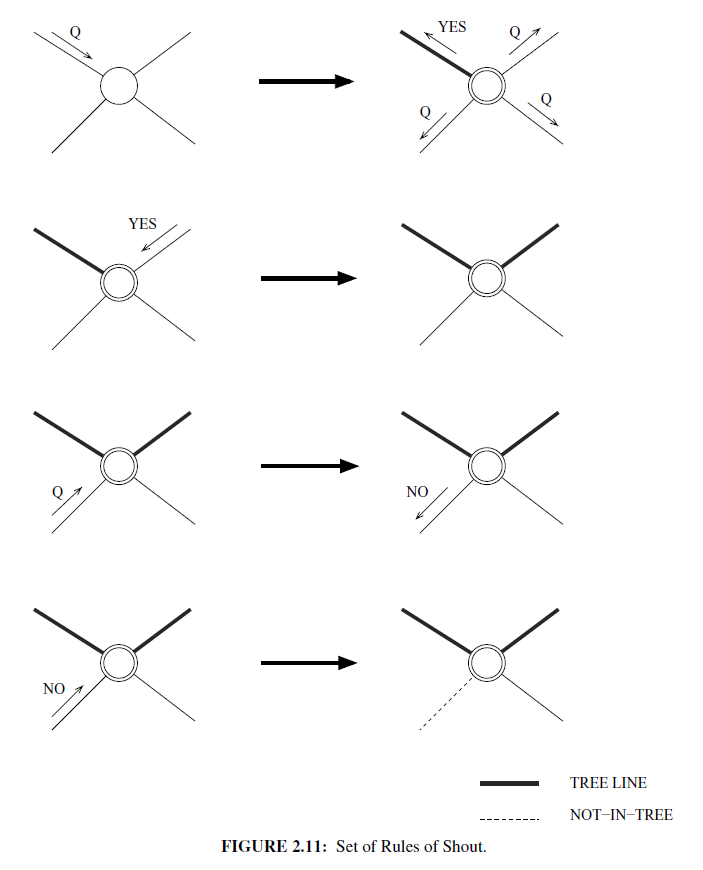
\includegraphics[width=15cm, keepaspectratio]{images/dddd.png}
\end{figure}

\subsection{Correttezza del protocollo}
Dimostriamo ora che dopo l'esecuzione del protocollo Shout si ha sempre uno ST radicato sul nodo iniziatore.\\
\theorem{
  Il protocollo \texttt{Shout} termina correttamente.
\begin{proof}
  Questo protocollo consiste nel Flooding del messaggio Q. Data la correttezza del Flooding, è garantito che ogni nodo riceverà la domanda, e che quindi risponderà SI o NO ad ogni Q che riceve. La terminazione segue proprio da questo. Per provare la sua correttezza bisogna dimostrare che il sotto grafo $G'$ definito dall'insieme $TREE\_NEIGHBORS$ è uno spanning tree di G, ossia è \textbf{Connesso}, \textbf{Contiene tutte le entità} e \textbf{Non contiene Cicli}.
  Osserviamo i seguenti tre punti:
  \begin{enumerate}
    \item \textbf{Connesso:} Se $x \in$ $T_N(y)$ allora $y \in$ $T_N(x)$ (poiché all'invio di un ``\texttt{SI}'' un'entità accetta di essere figlia e l'altra apprende di essere padre).
    \item \textbf{Contiene tutte le entità:} Se un'entità $x$ invia un "SI" ad $y$, allora $x \in T_N(y)$; inoltre è connessa all'iniziatore s da un cammino dove "SI" è stato inviato su ogni link. \\
    \textbf{Dim:} Supponiamo un nodo $x$ non raggiungibile dall'iniziatore $s$ dal grafo T indotto dalla relazione con il "padre". Questo significa che $x$ non ha mai inviato un messaggio di SI, ma questo implicherebbe che $x$ non ha mai ricevuto la domanda Q. Ma questo è impossibile per la correttezza del flooding, ogni entità ha per forza ricevuto il Q e quindi $x$ non può esistere.\\
    (Prof) Se per assurdo così non fosse, significherebbe che $x$ non ha mai inviato un "SI" ma ciò è assurdo per la correttezza del Flooding, poichè $x$ ha ricevuto sicuramente Q, e quindi ha inviato un \texttt{SI}. Quindi l'albero ottenuto dopo l'esecuzione sarà sicuramente connesso
    \begin{center}
      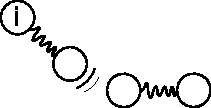
\includegraphics[scale=1]{images/n_21}
    \end{center}
    \item \textbf{Non contiene Cicli:} Ogni $x \neq $ \texttt{initiator} manda esattamente un solo messaggio ``\texttt{SI}''; se così non fosse, potrebbero essere presenti dei cicli che in un albero non possono essere presenti.
    
  \end{enumerate}
\end{proof}
}
Date queste supposizioni, il sottoinsieme $G'$ definito da tutti i $TREE\_NEIGHBORS$ contiene tutte le entità, è connesso e non contiene cicli. È possibile affermare che è uno Spanning Tree di G.\\
Si noti che G è in realtà un albero radicato nell'iniziatore. Ricordiamo che, in un albero radicato, ogni nodo (tranne la radice) ha un genitore: il vicino più vicino alla radice; tutti gli altri suoi vicini sono chiamati children. Il vicino a cui $x$ invia un $Si$ è il suo $genitore$; tutti i vicini da cui riceve un $Si$ sono suoi figli. Questo fatto può essere utile nelle operazioni successive.\\
L'esecuzione del protocollo Shout termina con la terminazione locale: ogni entità sa quando la propria esecuzione è terminata; questo si verifica quando entra nello stato \textit{done}.\\
Si noti tuttavia che nessuna entità, incluso l'iniziatore, è a conoscenza della terminazione globale (ovvero, ogni entità è terminata localmente). Questa situazione è abbastanza comune nei calcoli distribuiti. Se è necessario che l'iniziatore sappia che l'esecuzione è terminata (ad esempio, per avviare un'altra attività), Flood + Reply può essere facilmente modificato per raggiungere questo obiettivo.

\subsection{Costi}
Andiamo ora ad analizzare i costi del protocollo:

\underline{Messaggi:}
\begin{center}
  $M[$\texttt{Shout}$/RI] = 2 M[$\texttt{Flooding}$/RI] = 2(2m-n+1) = 4m - 2n + 2 = O(m)$
\end{center}
\begin{center}
  $M[$\texttt{Shout}$/RI] = 4m - (2(n-1)) = O(m)$
\end{center}
Dove:
\begin{itemize}
    \item 4m sono i 4 messaggi per arco dati i ritardi di comunicazione
    \item Ai 4m messaggi sottraggo tutti gli archi in cui passa un Q ed un SI, che sono appunto (n-1) + (n-1).
\end{itemize}

Questo perchè, se a seguito di una domanda rispondo "SI", sull'arco passano 2 messaggi, ma se invio "NO", per i ritardi di comunicazione, posso avere fino a quattro messaggi. Quindi ho 4 messaggi per arco, a cui sottraggo però gli 2(n-1) archi su cui passano (n-1) "SI" e (n-1) "Q".

\begin{center}
  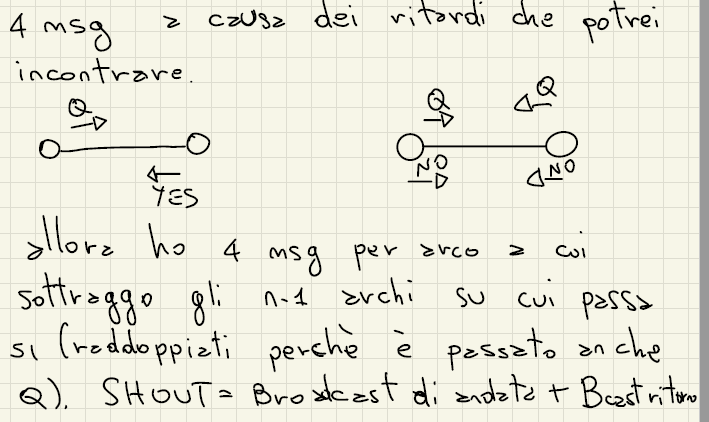
\includegraphics[scale=1]{aa/hh}
\end{center}

\underline{Tempo:}
\begin{center}
  $T[$\texttt{Shout}$/RI] = 1 + T[$\texttt{Flooding}$/RI] \leq d + 1 = O(d)$
\end{center}
Mandiamo i ``\texttt{SI}'' contemporaneamente ai $Q$; inoltre il $+1$ è per il \texttt{NO} che risponderà l'ultimo nodo nel caso peggiore in cui avesse già ricevuto la domanda Q da un'altra entità.

\begin{center}
  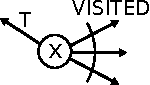
\includegraphics[scale=1]{images/n_22}
\end{center}

\subsection{Protocollo Shout}
\begin{lstlisting} [caption={\textit{Protocollo Shout.}}]
S = {INITIATOR, ACTIVE, IDLE, DONE}
Restrictions = RI

INITIATOR
    Spontaneously
    begin
        Tree-neighbours = $\emptyset$
        send(Q) to N(x)
        counter = 0
        become ACTIVE
    end

IDLE
    Receiving(Q)
    begin
        Tree-neighbours = {sender}
        send(YES) to sender
        counter = 1
        if counter = |N(x)|
        	become DONE
        else
        	send(Q) to N(x)\sender
        	become ACTIVE
    end

ACTIVE
    Receiving(Q)
    begin
        send(NO) to sender
    end
    
    Receiving(YES)
    begin
        Tree-neighbours =  Tree-neighbours $\cup$ {sender}
        counter = counter + 1
        if counter = |N(x)|
        	become DONE        
    end
    
    Receiving(NO)
    begin
       	counter = counter + 1
        if counter = |N(x)|
        	become DONE 
    end
    
\end{lstlisting}

\subsection{Complessità del problema: Lower Bound}
Vediamo ora quanto ci costa, in generale, la costruzione di uno Spanning Tree:

\underline{Messaggi:}
\begin{center}
  $M(ST/RI) \geq m = \Omega(m)$
\end{center}
\textbf{Dim del Lower Bound:} 
Assumiamo che esista un protocollo A corretto che, in ogni esecuzione sotto le restrizioni R ed UI, in ogni Grafo utilizza un numero di messaggi $<m$ per risolvere il problema della costruzione di uno spanning tree. Se cosi fosse ci sarebbe un arco in G dove non transitano messaggi in nessuna direzione durante un esecuzione di A. Consideriamo l'esecuzione di A in G e sia e=(x,y) l'arco dove non vengono trasmessi messaggi. Costruiamo ora un nuovo grafo G' da G ottenuto rimuovendo l'arco $e$ ed aggiungendo un nuovo nodo $z$ e due nuovi archi $e_1=(x,z)$ e $e_2=(y,z)$. Assumiamo che $z$ non sia iniziatore del protocollo. Eseguiamo ora la stessa identica esecuzione di A nel nuovo grafo G', dato che non transitavano messaggi tra x ed y è possibile eseguire la stessa esecuzione, poichè su G' il link tra x ed y nemmeno è presente. Però dato che nessun messaggio transitava tra x ed y, in G' nessun messaggio transita tra x e z e y e z, ma dato che z non è iniziatore e non riceve nessun messaggio, non invierà mai una risposta. Questo significa che in tempo finito il protocollo A termina, affermando che ha costruito una spanning tree di G' ma in questo caso z non è conneesso all'albero costruito, quindi A non termina correttamente.

\underline{Tempo:}
\begin{center}
  $T($\texttt{ST}$/RI) \geq d(G) = \Omega(d)$
\end{center}
Per raggiungere il nodo più lontano abbiamo bisogno di $d$ step.
Abbiamo quindi che Shout è ottimo sia in termini di messaggi ($\Theta(m)$, sia in termini di tempo $\Theta(d)$).

\section{Shout+ miglioramento di Shout}
Possiamo ridurre il numero di messaggi inviati rimuovendo i messaggi di tipo \texttt{NO}. Per ottenere questo possiamo fare in modo che la ricezione di un messaggio di tipo Q su un nodo che stà aspettando una risposta funzioni come "NO" implicito.\\
Prendiamo ad esempio un nodo $x$ che ha appena inviato un messaggio Q al suo vicino $y$.\\ Perchè $y$ potrebbe rispondere NO? \\Risponderà così solo se ha già ricevuto una domanda Q e quindi già risposto SI a qualche altra entità, in questo caso $y$ ha già inviato Q allo stesso tempo a tutti gli altri vicini, incluso $x$. Se $y$ risponde NO ad $x$, deve aver già inviato Q ad x. Possiamo ovviamente usare questa caratteristica a nostro vantaggio, dopo che $x$ invia Q ad $y$, se riceve SI sa che $y$ è un suo vicino, se invece riceve Q, dedurrà che $y$ ha risposto NO.\\
In altre parole, quando un messaggio Q arriva ad un nodo che sta aspettando una risposta può essere inteso come una risposta negativa, quindi concludiamo che è possibile non inviare messaggi di NO.
\begin{center}
  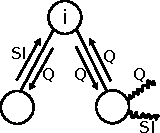
\includegraphics[scale=1.4]{images/n_23}
\end{center}
\underline{Messaggi:}\\
Su ogni arco viaggiano quindi le coppie di messaggi ($Q$,\texttt{SI}) o ($Q$,$Q$)

\begin{center}
  $M[$\texttt{Shout+}$/RI] = 2m$ (è effettivamente =)\\
\end{center}

\underline{Tempo:}\\ 
 Rispetto allo Shout risparmiano $1$, in quanto l'ultimo nodo non deve più attendere un'unità di tempo per ricevere i \texttt{NO} (non ci sono).
\begin{center}
  $T[$\texttt{Shout+}$/RI] \leq d$
\end{center}

\section{Algoritmo Shout+ con più iniziatori}
Abbiamo assunto fino ad ora che tutti i protocolli avevano iniziatore unico, ma come si comporterebbe il protocollo \texttt{Shout+} con più iniziatori?
\begin{center}
  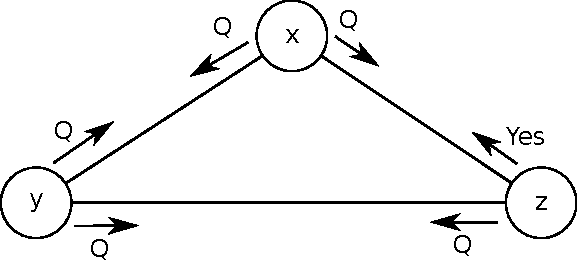
\includegraphics[scale=0.8]{images/n_36}
\end{center}
Quando su un arco viaggiano due domande, l'arco \underline{non} appartiene allo ST. \\
\texttt{Shout+} con più iniziatori \underline{non} funziona, perché \textbf{crea una foresta.}


\theorem{
  Il problema dello ST è deterministicamente non risolvibile sotto R (togliendo l'UI), ovvero che non esiste un protocollo deterministico che termina sempre correttamente in un tempo finito.
  \begin{proof}
  Per dimostrarlo prendiamo un grafo completo con 3 nodi ed etichettato come segue in figura.\\
    Supponiamo di avere un algoritmo deterministico A e più iniziatori:
    \begin{center}
      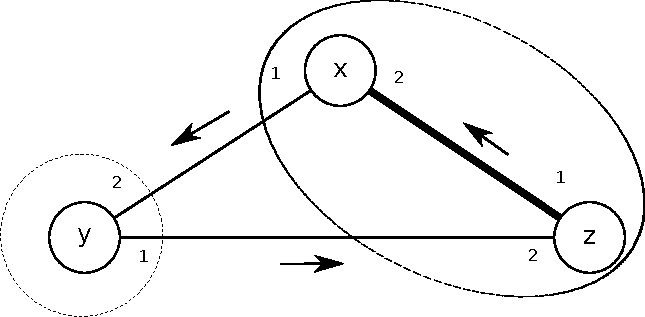
\includegraphics[scale=0.8]{images/n_37}
    \end{center}
    
    Supponiamo che $x, y, z$ siano tutti e tre iniziatori, che siano nello stesso stato, che inizino contemporaneamente il protocollo e che abbiano tutti valori identici. Se A è un protocollo che da soluzione al problema, dovrà funzionare sotto ogni condizioni di ritardo di messaggi e indipendentemente dal numero di iniziatori. 
Supponiamo di avere ritardo di comunicazione unitario, che sia presente la sincronia di Clock e che tutte le entità inizino contemporaneamente l'esecuzione del protocollo A. Dato che sono in stati identici (stessi valori iniziali e stessi numeri di porta), le entità eseguiranno le stesse computazioni, ottenendo gli stessi risultati (continuando ad avere gli stessi valori locali), inviare gli stessi messaggi agli stessi numeri di porta ed entrare eventualmente nel nuovo stato tutte insieme. In pratica tutte le entità continueranno ad essere completamente identiche. Se A da soluzione al protocollo, deve terminare in tempo finito. Nel nostro caso A dovrà solamente eliminare un arco per far si che si ottenga uno Spanning Tree; prendiamo per esempio l'arco (x,y). In questo caso la variabile Tree-neigbors sarà la porta con la label 2 dell'entità x e la porta 1 dell'entità y, invece z ha come Tree-neigbors porta \{1,2\}. In altri termini, quando il protocolli termina, tutte le entità hanno differenti valori per la variabile locale "Tree-Neighbors" ma questo è impossibile poichè per supposizione gli stati delle entità devono essere necessariamente identici.\\
    
    %Siccome $x, y, z$ hanno la stessa esecuzione e partono dallo stesso stato, in ogni momento, calcoleranno sempre lo stesso risultato e saranno quindi sempre nello stesso stato; quindi alla fine abbiamo o che tutti gli archi appartengono a ST, o nessuno. Ciò è \textbf{assurdo}.

  \end{proof}
}

\textbf{Causa del fallimento}\\
La causa per cui il protocollo Shout con più iniziatori fallisce è che un'entità non riesce a distinguere tra le varie richieste che gli vengono inviate. Quindi il più semplice approccio sarebbe quello di aggiungere un id ad ogni messaggio di "Q" e "Yes" così da identificarle.

Dobbiamo trovare l'insieme di restrizioni "minimo" (oltre a R) che ci permetta di costruire correttamente lo ST con più iniziatori.

\section{Spanning Tree con valori iniziali delle entità distinti}
Possiamo risolvere il problema aggiungendo una singola restrizione all'insieme R: ogni entità ha un valore iniziale unico (id) che permette di distinguerla dalle altre.
Quando un'entità invia un messaggio invia anche l'id dell' iniziatore.
\begin{center}
  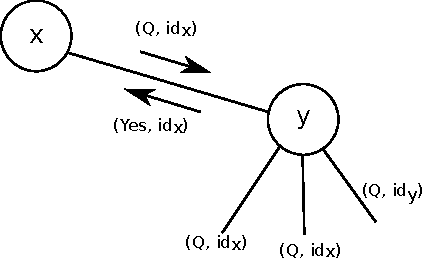
\includegraphics[scale=0.8]{images/n_38}
\end{center}
L'applicazione di questo approccio risulta nell'avere ogni iniziatore che costruisce il proprio spanning tree radicato in lui e che utilizza l'id degli altri iniziatori per distinguere tra le diverse costruzioni. Quindi invece che cooperare per la costruzione di un singolo spanning tree, si avranno contemporaneamente più spanning tree indipendentemente costruiti. Questo implica che  tutti i messaggi del protocollo (Ovvero messaggi di "Q" e messaggi di "Yes" nel protocollo Shout+) abbiano l'id dell'iniziatore. Sono richieste inoltre variabili addizionali poichè in ogni entità saranno presenti più istanze della variabile $TREE\_NEIGHBORS$, ovvero uno per ogni spanning tree che sta venendo costruito. Inoltre, ogni entità sarà in un differente stato per ognuna di queste costruzioni. Ricordiamoci che il numero di iniziatori non è noto a priori e può cambiare ad ogni esecuzione.
In questo modo costruiamo $K^*$ ST con $K^*=$ numero di iniziatori. Siccome \texttt{Shout+} ci costa $2m$, il costo è:

$$2m K^* = O(n^3)$$

poiché $1 \leq K^* \leq n$. %e poichè si sta costruendo non uno ma ma K* ST.

Ogni nodo può distinguere a quanti ST sta partecipando in base all'id dei messaggi.

\subsection{Algoritmo MultiShout}
Consideriamo adesso un algoritmo basato sul protocollo \textbf{Shout+} con un metodo migliore:
Un approccio migliore è quello di lasciare ad ogni iniziatore la possibilità di costruire il suo ST, ma di scegliere di far sopravvivere localmente solamente la costruzione con id \underline{minimo}. Quando un'entità si interfaccia con differenti costruzioni di uno ST, sceglierà sempre quella con id minore e terminerà quelle che conosce. I vantaggi di questo approccio sono:
\begin{enumerate}
    \item Ogni entità è coinvolta in una singola costruzione di uno ST.
    \item In terminazione, tutte le entità avranno un singolo ST in comune.
\end{enumerate} 

Gli stati di questo protocollo sono IDLE, ACTIVE e DONE. Tutte le entità iniziano in stato di IDLE ed in terminazione tutte le entità saranno in stato di DONE. 

Riassumendo quindi, quando un nodo x avente $id_x$ riceve un messaggio con $id_y$ tale che:

$$ id_y < id_x$$

Allora x smette di lavorare per l'entità a cui stava portando avanti la costruzione dello spanning tree e porta avanti la costruzione dello spanning tree radicato in y.
Il punto fondamentale di questo approccio è che solo lo ST con id minimo viene portato a termine tra gli iniziatori, quindi \texttt{MultiShout} costruisce un albero radicato sull'iniziatore con id minimo. Di conseguenza, i nodi conservano solo i dati relativi ad un singolo ST.\\
Per come si è costruito il protocollo però, quando un'entità ha concluso la sua costruzione, non sa se dovrà iniziare a lavorare nuovamente per qualcun altro, in quanto è possibile che un'entità che abbia terminato riceva un messaggio da un altro iniziatore (con la possibilità di avere id minore). Quindi è necessario includere nel protocollo un meccanismo che permetta la terminazione locale delle entità.
\\
\textit{Problema del protocollo:} \textbf{i nodi non hanno conoscenza locale di terminazione:} una possibile soluzione è fare in modo che le foglie dell'unico ST che viene portato a termine mandino al proprio padre un messaggio di fine lavoro fino alla radice, la quale diventa cosciente della fine del suo lavoro ed invia un messaggio di terminazione in broadcast. Possiamo vedere questo passaggio come un:
$$\textit{Convergecast + Broadcast}$$


\theorem{
Il protocollo MultiShout costruisce un ST radicato nell'iniziatore con id più piccolo tra gli iniziatori.
}
\begin{proof}
Sia s l'inizializzatore con id minore, consideriamo un altro iniziatore x diverso da s.
Da x verrà costruito quindi lo spanning tree radicato in lui, che chiameremo $T_x$. Dimostriamo due punti fondamentali:
\begin{enumerate}
    \item \textbf{La costruzione di $T_x$ non verrà completata:} Osserviamo che $T_x$ deve contenere tutti i nodi, incluso s, ma quando s riceve un messaggio relativo alla costruzione di un altro ST, avendo id minore di tutti, ignorerà il messaggio uccidendo la costruzione di quell'albero.
    \item \textbf{La costruzione di $T_s$ verrà completata:} Dato che l'id di s è il minore di tutti, nessuna entità ignorerà il messaggio e quindi lo ST sarà completato.
\end{enumerate}
\end{proof}

\subsubsection{Complessità}
Supponiamo di avere $K^*$ iniziatori connessi ognuno con un solo nodo nel sotto grafo $k_{n-K^*}$ completamente connesso (completo).
\begin{center}
  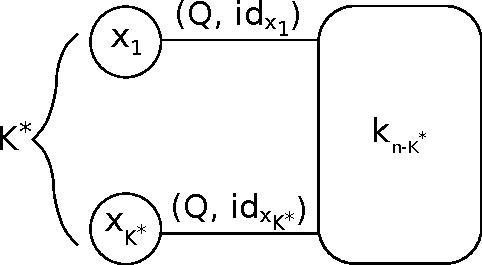
\includegraphics[scale=0.9]{images/n_39}
\end{center}
Inoltre, con $id_{x_1} > id_{x_2} > \cdots > id_{x_{K^*}}$.

Supponiamo adesso un'esecuzione dove i messaggi Q che inviano i $K^*$ iniziatori arrivano sul grafo completo in un ordine in base al loro indice, quindi $x_1$ arriva per primo, poi $x_2$ arriva per secondo e così via. Quando il messaggio $Q$ di $x_1$ arriva negli $n-K^*$ nodi, si genererà la costruzione dello spanning tree radicato in lui. Assumiamo adesso che prima che il messaggio $Q$ di $x_2$ arrivi nel grafo completamente connesso, la computazione di $x_1$ dentro il suddetto grafo sia conclusa, pagando quindi $O(n-k^*)^2$. Quando $Q$ di $x_2$ arriva nel grafo completamente connesso, tutto il lavoro precedentemente svolto da $x_1$ è da buttare via, poichè tutti i nodi adesso devono seguire la sua costruzione dello ST, avendo id più piccolo di $x_1$. Se si continuasse in questo modo, $O(n-k^*)^2$ verrebbe ripetuto per $K^*$ volte, per un totale di:

%Supponiamo ora che $x_1$ parta per primo e che inizi a costruire uno ST in $k_{n-K^*}$ pagando $2m = O(n^2)$. Assumiamo adesso che la costruzione dello ST radicato in $x_1$ sia conclusa (pagando quindi $O(n-k^*)^2$) prima che il messaggio Q di $x_2$ venga spedito all'interno del suddetto grafo. Tutto il lavoro fatto da $x_1$ è da buttare, poichè adesso i nodi dovranno seguire la costruzione dello spanning tree radicato in $x_2$. Si va avanti così fino a $x_{K^*}$, disfacendo di volta in volta il lavoro precedente.

\underline{Messaggi:}
\begin{center}
  $M[$\texttt{MultiShout}$] = O(k^*(n-k^*)^2)) + (n-1)+ (n-1) = O(n^3)$\\
  con $k$ frazione lineare rispetto ad $n$, ad esempio $k=\frac{n}{2}$
\end{center}
$k^*$ volte invio un messaggio in un grafo completo (archi = $m^2$) dato che $m=n-k^*$. E (n-1), (n-1) è per Convergecast e Broadcast in un albero (un messaggio per nodo).

\underline{Tempo:}
\begin{center}
  $T[$\texttt{MultiShout}$] \leq d + 1 + 2d = 3d + 1$
\end{center}
Dove:
\begin{itemize}
    \item  $d+1$ è il tempo speso per la costruzione dello ST attraverso il protocollo Shout
    \item $2d$ è il costo del Broadcast e Convergecast che parte dal minimo necessario per la terminazione del protocollo
\end{itemize}
%il $2d$ è per il tempo speso per effettuare il convergecast e broadcast del minimo finale, mentre lo $d+1$ è il tempo speso da normale protocollo di shout per la creazione dello ST.

\section{ST con altri protocolli e Iniziatore Unico}
Possiamo costruire uno Spanning Tree usando protocolli che risolvono il problema del Broadcast o dell'Attraversamento, opportunamente modificati.

\subsection{ST con Traversal normale DF}
Sappiamo che l'applicazione del protocollo $DF$ costruisce già effettivamente uno Spanning Tree del grafo che stiamo considerando. Questo è ottenuto rimuovendo gli archi dove transita un messaggio di BACKEDGE da G. In altre parole, l'insieme Tree\_Neighbors di un'entità $x$ saranno tutte le entità dalle quali riceverà un messaggio di RETURN, e se $x$ non l'iniziatore (poichè siamo su Iniziatore Unico come Restrizione), l' entità dalla quale $x$ ha ricevuto T per la prima volta.

\subsection{ST con Traversal normale DF*}
Il protocollo utilizza una visita in \textit{profondità}, quindi se ad esempio lo facessimo girare su un grafo completo (quindi $d(G)=1$) mi darebbe un output uno Spanning Tree dove $d(T) = n-1$. Visto che il nostro scopo è quello di costruire un albero di copertura per far girare i protocolli visti, e questi hanno complessità temporale che dipende dal diametro della rete, impiegherebbero un tempo elevato per il raggiungimento dell'obiettivo. Il nostro scopo è quello di avere $d(T) \leq 2d(G)$. Infine, il numero di messaggi da utilizzare per la costruzione dell'albero risulta essere troppo alto per i nostri scopi (circa $4m$).

\subsection{ST con Broadcasting}
\theorem{L'esecuzione di qualsiasi protocollo di Broadcasting costruisce uno Spanning Tree.}
Prendiamo un qualsiasi protocollo di broadcasting B. Da come abbiamo definito il broadcast, tutte le entità riceveranno l'informazione $I$ che inizialmente ha solo l'iniziatore.


Visto che i protocolli che utilizzano la DFS ci costruivano alberi ``alti``, proviamo ad utilizzare la visita in \textit{ampiezza}.

\subsubsection{BFS}
Per la costruzione dello Spanning Tree tramite la BFS, utilizziamo la seguente strategia.
\textbf{Strategia:}
\begin{enumerate}
  \item determinare il nodo con eccentricità minore (quello che detta l'eccentricità di $G$, ossia il \textit{nodo centrale});
  \item costruire un BF-ST radicato su tale nodo.
\end{enumerate}

\begin{center}
  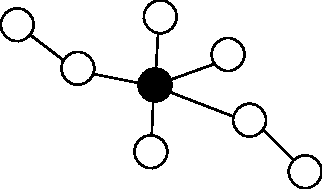
\includegraphics[scale=1]{images/n_24}
\end{center}

\subsubsection{Eccentricità}
In un nodo x: 
$r_G(x) = max\{ \delta_G(x,y), y \in V(G) \}$ [ECCENTRICIT\`{A} DEL NODO]\\
In un grafo: $r(G) = min \{ r_G(x), x \in V \}$. Il nodo \emph{x} con eccentricità minima in G è detto \textbf{centro di G} (in un grafo completo sono tutti centri).\\

Se si fa una BFS partendo da un centro (possono essere molteplici) otteniamo lo ST più basso possibile.\\
Infatti tale albero avrà altezza $r(G)$, possiamo quindi dire che: $2 d_G \geq d_{BFS} \geq d_G$.
%Ove $d_G$ è il diametro del grafo [\ref{def_diametro}].

Per costruire uno ST con BFS, sotto restrizioni di iniziatore unico si può fare nel seguente modo:\\
Iniziatore manda un messaggio in broadcast ai vicini e attende la risposta\\
Quando l'iniziatore ha avuto tutte le risposte rinvia un messaggio (tipo TOKEN)\\
L'entità che lo riceve fa partire la costruzione nel nuovo livello come visto sopra e poi rinvia il TOKEN all'iniziatore che lo invierà al fratello.

Il costo è $\mathcal{O}(n^2)$, considerando i seguenti tipi di messaggio:\\
$Q \leftarrow 2m - n +1$\\
$YES, NO \leftarrow 2m -n +1$\\
$T \leftarrow 2n r(g)$



\chapter{Esplorazione di un grafo anonimo}
Per questo capitolo si fa riferimento al seguente paper: \emph{D. Ilcinkas - Setting Port Number For Fast Graph Exploration}

Affrontiamo adesso il seguente problema: \textbf{Vogliamo inserire dei numeri di porta in modo tale che un robot esplori sequenzialmente un grafo in modo periodico (cioè ricominci quando ha finito) utilizzando il percorso minimo.} %e vogliamo che ci metta meno tempo possibile, ovvero che il percorso sia minimo.}

Specifichiamo il robot come un'\textbf{automa di Mealy}.

Il grafo in input ha topologia incognita ed il robot ha \textbf{orientamento locale} ovvero le etichette sugli archi uscenti dal nodo $v$ sono distinti e con valori:
\begin{center}
$1, \cdots, d_v = \deg (v)$\end{center}
\begin{center}
   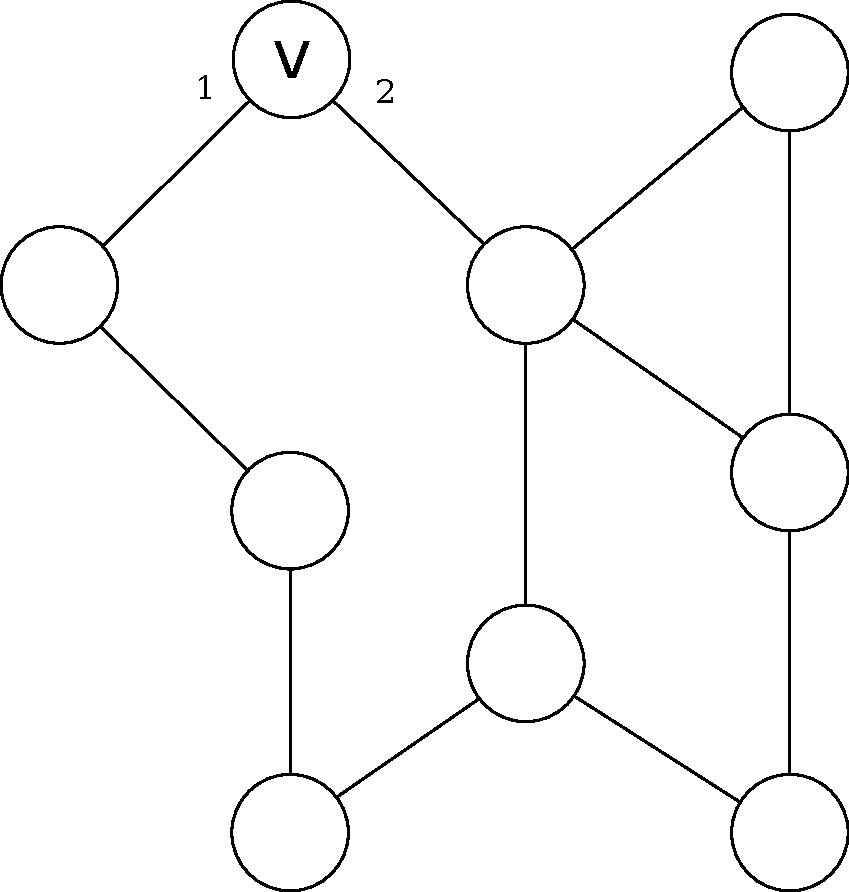
\includegraphics[scale=0.3]{images/n_25}
\end{center}

Per il robot dobbiamo specificare la \textbf{funzione di transizione}:\\\\
\begin{center}
 $f(s,i,d_v) = (s',i')$
\end{center}

Dove:
\begin{itemize}
 \item $s$ = stato in cui sono;
 %\item $i$ = porta in cui esco.
 \item $i$ = porta in cui entro nel nodo $v$ in cui vado.
 \item $d_v = \deg(v)$ Grado del nodo in cui arrivo.
 \item $s'$ = stato in cui vado una volta entrato in $v$;
 \item $i'$ = porta in cui esco quando sono su $v$.
\end{itemize}

La scelta migliore sarebbe trovare uno Spanning Tree del grafo incognito che stiamo considerando, in questo caso la lunghezza ($\Pi$) sarebbe $\Pi(n) = 2(n-1)$ dove:
\begin{itemize}
    \item 2 indica il dover scendere e risalire il grafo (stiamo attuando una DFS)
    \item n-1 indica il numero dei nodi dell'albero
\end{itemize}
\textbf{Perchè il lower buond del problema è n?}\\
L'OverBound del problema dovrebbe essere esattamente $\Omega(n)$ e non $2n$, ovvero si devono necessariamente attraversare tutti i nodi. Troviamo un percorso di lunghezza $\Pi$ pari ad $n$ su un Anello, per esempio, o se esiste nel grafo considerato un sottografo che è un anello, per poi etichettarlo in maniera tale da entrare sempre da porta 1 ed uscire sempre da porta 2. Il problema è che non sono sicuro che questo ciclo esista sempre. I grafi in cui è presente un ciclo al loro interno sono detti Hemiltoniani, ma sapere se un grafo è Hemiltoniano è un problema NP-completo. Ovvero:\\ Dato un grafo G trovare un sotto ciclo che tocchi tutti i nodi del grafo G passando solamente una volta per ogni arco e che ritorni al nodo di partenza.\\
Dato che questa strada è complessa scelgo di costruire prima uno Spanning Tree del grafo e poi far muovere l'automa li dentro, anche se passa più volte per arco.
\\\textbf{Un esempio di un grafo che non ammette ciclo emiltoniano è un qualsiasi grafo avente almeno un nodo con grado uno.} Poichè arrivati in quel nodo si deve necessariamente tornare indietro e quindi passare per un arco due volte. Dato che si vuole costruire uno Spanning Tree, ci sarà necessariamente un nodo di grado uno. Quindi è necessario tenere $2(n-1)$ come lowerBound e non $n$.

\subsection*{Risultato di impossibilità}
Non è possibile risolvere il problema di esplorazione periodica di un grafo se i numeri di porta sono dati arbitrariamente (se i numeri di porta sono specificati da un avversario, è facile far entrare l'automa in loop).

Nel 2006 Dobrev ha dato un upper bound al problema, pari a $10n$, usando la \textbf{regola della mano destra} ed usando \textbf{automa ad oblio} (non cambiano stato e ne ha solo uno):
\begin{center}
 $f(s,i,d) = (s,(i~mod~d) + 1)$
\end{center}
L'automa quindi uscirà su porta 1 quando la i è pari al grado (d) del nodo.

\section{Come possiamo migliorare il bound di 10n?}
%Abbiamo esplorato tutti i nodi ed il robot torna nel nodo di partenza, uscendo dalla porta di partenza. Nel nostro caso 
Consideriamo che l'automa abbia \textbf{memoria finita} nella quale non sono memorizzati i numeri di porta, poichè in un grafo qualsiasi non conosciamo il deg massimo.

Il periodo trovato è:
\begin{center}
 $\pi(n) \leq 4n-2$ 
\end{center}
Per questo miglioramento sono necessari 3 stati, aggiungere stati equivale ad aggiungere memoria all'automa. L'obiettivo è quello di costruire uno spanning tree in modo da risparmiare la visita di alcuni archi inserendo opportunamente i numeri di porta. \\
Fondamentale il fatto che posizioneremo dei numeri di porta in maniera tale che se esco da porta $i$ e quell'arco non è appartenente allo Spanning Tree, allora nessun altro arco con porta maggiore di $i$ sarà appartenente allo spanning tree. Questo è utilizzato dall'automa per evitare di testare troppi archi durante l'attraversamento.

\section{ST con Orientamento Locale:}
Consideriamo un generico spanning tree di G, chiamato $T$.
\begin{itemize}
    \item Sia $F \subseteq E$ il sottoinsieme di archi appartenenti all'albero $T$.
    \item $\forall v \in V$, $F_v$ denota l'insieme degli archi incidenti a $v$ in $T$.
\end{itemize}

\definition{un \textbf{orientamento locale} degli archi di un grafo è detto \textbf{compatibile} con un ST $T=(V,F)$ se e solo se:
\begin{enumerate}
 \item $\forall e \in E$, almeno uno dei suoi numeri di porta è 1 se e solo se $e \in F$;
 \item $\forall v \in V$ gli archi appartenenti allo ST ($F_v$) hanno i loro numeri di porta da 1 a $|F_v|$.
\end{enumerate}
}
 \textbf{Prima di poter far girare l'automa su un grafo, bisogna sia costruire uno spanning tree sia definire un orientamento locale. L'algoritmo Small-Ports permette di fare entrambe le cose insieme.}

\section{Algoritmo Small-Ports per la costruzione dello ST con orientamento locale}
Questo algoritmo permette di costruire un orientamento locale dato in input uno Spanning Tree, che permetterà al Robot di poter risolvere il problema proposto ad inizio capitolo.
\begin{enumerate}
 \item Come input si ha uno Spanning Tree $T$ di un grafo generico $G$. Sia $r$ la sua radice.

 \item $\forall v \neq r$, assegna la porta 1 all'arco di $T$ che conduce ad $r$. In $r$, assegna 1 ad un qualunque (quindi scelto arbitrariamente) arco in $F_r$.
 \item $\forall v$, assegna arbitrariamente le porte da 2 a $|F_v|$ (che indica da 2 al grado del nodo $v$) ai rimanenti archi $F_v$ (appartenenti a T quindi) se esistono.
 \item Infine $\forall v$, assegna arbitrariamente i numeri di porta da  $|F_v|+1$ a $d_v$, agli archi a cui non sono ancora stati assegnati dei numeri di porta, se esistono.% quindi i rimanenti archi non appartenenti a T, se esistono.
\end{enumerate}
\textbf{Spiegazione dei punti precedenti a parole:} I primi due punti sono intuitivi, il terzo invece fa sempre riferimento al fatto che vanno assegnati i numeri di porta più piccoli agli archi dove nell'altra estremità c'è porta 1, ovvero archi sempre appartenenti allo ST. Il quarto si riferisce all'inserimento dei numeri di porta di tutti gli archi che nell'altra estremità non hanno porta 1 e quindi non sono appartenenti allo ST.

Date queste regole quindi, qualora si uscisse da una porta con etichetta 1 allora siamo sicuri che si è attraversato un arco appartenente allo ST. Se così fosse però molto probabilmente ( a meno che il nodo su cui andiamo non abbia cardinalità = 1) non avrà anch'esso porta 1, e quindi bisognerà testare quale dei suoi archi uscenti è quello appartenente allo ST.

\example{
\begin{center}
   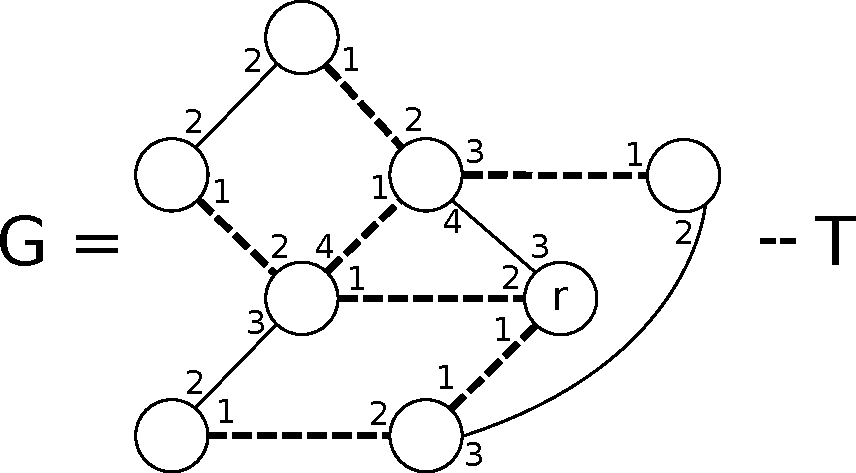
\includegraphics[scale=0.6]{images/n_26}
\end{center}
}

È un orientamento locale in quanto $\forall v \in V$ tutte le etichette vanno da 1 a $d_v$.

È compatibile con $T$ poiché valgono \textit{i)} e \textit{ii)}.

Otteniamo quindi uno e un solo arco con etichette entrambe 1, il quale non ci consente di dire quale dei due nodi estremi è la radice.
Abbiamo ottenuto quindi uno Spanning Tree con orientamento locale. Andiamo a definire come si dovrà muovere l'automa su di questo.
%\subsection*{Complessità}
%\begin{itemize}
% \item Passo 1: $=(m \log n)$
% \item Passo 2: $O(n)$
% \item Passo 3 + Passo 4: $2m -n$
%\end{itemize}
%Quindi la complessità totale è di $m \log n + 2m$.

\section{Funzione di transizione}
Trovato lo Spanning Tree del nostro grafo di partenza attraverso il corretto inserimento dei numeri di porta, analizziamo i movimenti del robot. Esso si basa su tre stati:
\begin{itemize}
\item Normal, l'automa sta percorrendo per certo un arco in T
\item Test, percorre un arco che può o meno essere in T
\item Backtrack, percorre un arco che sicuramente non è in T
\end{itemize}
\subsection{N: Normal}
\begin{center}
  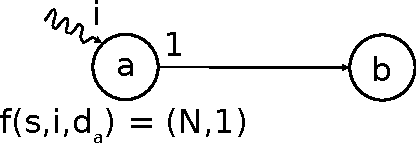
\includegraphics[scale=0.7]{images/n_27}
\end{center}
%Per la regola numero 2 definita precedentemente (quella dell'inserire etichetta 1 sempre nell'arco che va verso la radice), se esco da $a$ su porta 1, allora $b$ è il mio padre nello ST, quindi il robot esce in stato $N$, in quanto quell'arco è sicuramente appartenente allo ST. Abbiamo che \textbf{d} = Grado del nodo corrente e \textbf{i} = Porta d'ingresso.
\begin{equation}
  f(N,i,d) =
  \left\{
  \begin{array}{r
      @{\quad{\mbox{se}}\quad}
      l}
    (N,1) & i = d \\
    (T,i+1) & i \neq d \\
  \end{array}
  \right.
\end{equation}

\begin{itemize}
    \item Se la porta in cui entro su $v$ è esattamente uguale al suo grado, allora esco attraverso porta 1 in stato di Normal.
    \item Se invece il numero di porta in cui entro su $v$ è diversa dal suo grado allora cambio stato in Testing e mi muovo sull'arco avente porta $i+1$
\end{itemize}.

 %Se il nodo ha solo un arco (d = 1) allora sicuramente quello è appartenente allo ST, quindi esco nello stato di Normal su porta 1. Se invece la porta in cui entro (i) è diversa dal grado del nodo corrente dovrò cambiare stato in TEST. Questo metodo implementa una visita di $T$ in profondità.

\subsection{T: Test}
\begin{center}
  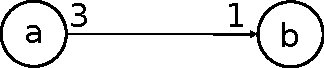
\includegraphics[scale=0.7]{images/n_28}
\end{center}

Se esco da $a$ su una porta diversa da 1 vado in stato $T$. Se trovo un valore 1, allora quell'arco è appartenente allo ST.

\begin{equation}
  f(T,i,d) =
  \left\{
  \begin{array}{r
      @{\quad{\mbox{se}}\quad}
      l}
     (N,1) & i = d = 1 \\
     (T,i+1) & i = 1 ~\textrm{e}~ d \neq 1 \\
     (B,i) & i \neq 1 \\
  \end{array}
  \right.
\end{equation}
\begin{itemize}
    \item Esco su porta 1 in stato N se trovo che $v$ ha come grado 1 e la porta in cui entro su $v$ è proprio 1.
    \item Esco su porta $i+1$ ancora in stato $T$ se trovo ancora porta 1 nel nodo in cui vado ma il grado di questo nodo è diverso da 1.
    \item Cambio in stato in BackTrack e attraverso porta $i$ se trovo porta diversa da 1 sul nodo in cui sono andato.
\end{itemize}


\subsection{B: Backtrack}
\begin{center}
  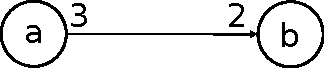
\includegraphics[scale=0.7]{images/n_28-2}
\end{center}

\begin{center}
  $f(B,i,d) = (N,1)$
\end{center}

\begin{itemize}
    \item Se mi posiziono su $v$ in stato di BackTrack allora cambio stato in Normal e attraverso porta 1, ovvero un arco che è sicuramente appartenente allo ST.
\end{itemize}

\subsection{Complessità}
\textbf{Perchè è $\Pi(n) \leq 4n$ il costo?} Questo equivale a chiedersi quanto vale il periodo $\Pi(n)$\\

L'automa deve esplorare in profondità tutto T andata e ritorno, spendendo quindi $2(n-1)$, a cui poi devo sommare i vari errori commessi dall'automa; può commettere 1 errore su ogni nodo ma può sbagliare su tutti, quindi $n$. Sbagliando deve anche tornare indietro, che è un altra aggiunta di $n$ errori. Quindi si avrebbe in totale: $2(n-1)+n+n = O(4n) $ o anche $\leq 4n$.
Se il grafo è un \textbf{albero} siamo ottimi, poichè il lower bound è anch'esso $n$.\\
In caso di \textbf{grafo completo} non posso esplorare l'albero convenientemente a meno che non si parta dalla radice, in quel caso usando solo 2 stati si avrebbe costo = $2n-2$.
Potrei però costruire un grafo $G'$ ring, in quel caso sempre con 2 stati si avrebbe un costo = $n$.
Purtroppo l'idea del ring si può applicare solo su grafi che siano Hamiltoniani (dotati di un cammino che tocca tutti i nodi una e una sola volta), ma sapere se un grafo è Hamiltoniano è un problema NP-completo.

Concludiamo quindi che il lower-bound è $2n-2$, esclusi i grafi Hamiltoniani.

\section{Prova formale della correttezza}
\textbf{Enunciato: } Sia G un grafo di dimensione $n$ con orientamento locale compatibile con uno spanning-tree T.
Se l'automa A inizia da un qualunque nodo in un qualunque stato, dopo al più 2 step A entra in un cammino chiuso P e lo percorre per sempre. Inoltre P è di lunghezza al più $4n-2$ e contiene tutti i nodi di G.
\begin{proof}
 \_
\begin{itemize}
    \item Sia G un grafo con n nodi;
    \item Sia $v$ un nodo arbitrario di G;
    \item Sia $e$ un arco dello ST di $v$ con porta 1.
\end{itemize}
Consideriamo ciò che otteniamo rimuovendo tale arco, il nostro T avrà allora 2 sotto alberi, quello che contiene $v$ lo chiameremo $T_1$ e con $n_1$ indichiamo il numero di nodi in $T_1$.

Per dimostrare l'enunciato useremo la seguente proprietà:\\
\textbf{Claim: } Se A entra in $v$ attraverso porta 1 in uno stato differente da B allora prima o poi lascerà $v$ attraverso porta 1 nello stato N. Inoltre, tra questi 2 eventi, esplora tutti i nodi di $T_1$ in al più $4n_1 - 2$ step, e non esce da nessun nodo non in $T_1$ attraverso porta 1 durante l'attraversamento.
\begin{proof}
Per poter provare il Claim ci si focalizza sul sottoalbero $T_v$ ottenuto tagliando l'arco con etichetta 1. Si prova quindi Per induzione sull'altezza di $T_n$:
\begin{itemize}
    \item Base: $h(T_1) = 0 \Rightarrow v$ \textbf{è} una foglia in T.
        \begin{itemize}
            \item Se v è una foglia anche su G, allora l'automa lascia automaticamente la foglia $v$ attraverso porta 1 in stato N ed il claim è dimostrato. Questo avviene perchè $d=i$ quindi si va sullo stato N.
            \item Se invece il $d(v)>1$ su G, l'automa entra in $v$ in testing $(T, i+1)$ ed attraverserà l'arco con etichetta 2. $v$ è una foglia su T, e dato che $e$ è in T, $e'$ non può esserlo, quindi la porta nell'altro estremo non potrà mai essere 1. Quindi tornerà indietro con B. In questo caso avremo 2 step, derivati da $(4n_1 -2)$ con $n_1=1$ 
        \end{itemize}
    \item Passo induttivo: $v$ \textbf{non} è una foglia in T.
    \begin{itemize}
        \item La porta "2" che è quella che l'automa attraverserà una volta posizionato su $v$, ci conduce ad una porta "1". Se andiamo a considerare il sotto albero $T_2$ radicato in questo nodo avremo:\\
        $h(T_2) \leq h(T_1) -1$, poichè si effettua uno step in profondità dal nodo v al sottoalbero ottenuto tagliando l'arco con etichetta 1.
        Possiamo quindi applicare l'ipotesi induttiva e avremo che in $4n_2-2$ step verrà visitato $T_2$.
        Ora l'automa torna in $v$ nello stato N, la scelta che seguirà dipende dal grado di $v$. Supponiamo $p$ la label più grande di un albero radicato in $v$; in generale avremo che per tutti gli archi con porta $i \leq p$ l'automa esplorerà l'albero $T_i$ in al più $4n_i - 2$ passi.\\
        \textbf{Quanti passi in totale effettua l'automa nei sotto alberi?}
    \end{itemize}
\end{itemize}
\begin{equation}\nonumber
\begin{split}
\#Step & \leq \sum_{i=2}^{p} (4 n_i - 2 +2) +2= 4\sum_{i=2}^{p} (n_i)+2  = 4(n'-1)+2 = 4n'-2
\end{split}
\end{equation}

\begin{itemize}
    \item $(4 n_i - 2)$ Sono i passi per esplorare il singolo sotto grafo.
    \item +2 dentro la parentesi sono i passi che l'automa fa verso il sotto grafo per poi tornare al nodo di partenza.
    \item +2 fuori dalla parentesi sono i passi che l'automa fa qualora ci fosse una porta che non conduce ad un sotto albero con porta 1 dall'altra parte. L'errore lo fa a porta $p+1$, infatti la sommatoria arriva fino a $p$.
    \item Dopo il primo $=$, $\sum_{i=2}^{p} (n_i)$ sono tutti i nodi del sotto albero T' tranne $v$, che sono infatti $(n'-1)$.
\end{itemize}

\begin{comment}


%Questi sono i passi che fa l'automa in ogni sotto albero. A questi vanno aggiunti anche i passi per raggiungere i sotto alberi e esattamente 2 step qualora ci fosse un altro arco che non ha 1 nell'altra estremità.
\begin{equation}\nonumber
\begin{split}
\#passiTot & = \sum_{i=2}^{p} 4 n_i -2 + 2(P-1) + 2 = \\
           & 4 \sum_{i=2}^{p} n_i -2 - 2(P-1) + 2(P-1) + 2 =\\
           & 4 \sum_{i=2}^{p} n_i =  4(n'-1) +2 = 4n'-2
\end{split}
\end{equation}


Dove:
\begin{itemize}
    \item $\sum_{i=2}^{p} n_i = (n'-1)$ fa quel valore perchè sono tutti i nodi nei rispettivi sotto alberi, che vengono chiamati $n'$ -1 invece è perchè la sommatoria inizia da 2 e quel -1 è esattamente il nodo $v$.
    \item La sommatoria indica tutti quelli che hanno porta 1 alla fine del link (nell'esempio sul quaderno erano $T_i, T_j, T_p$)
    \item $4n_i - 2$ Indica tutti quelli dentro al sottografo (numero di passi per attraversare tutti i nodi)
    \item $2(P-1)$ Tutti i passi da V ai sottografi (quelli tagliati) e viceversa. P indica tutti i vicini di V e -1 poichè è l'arco in entrata "dall'alto".
    \item +2 Se c'è qualche altro link oltre a P che non ha dall'altra parte etichetta 1, ed indica andare in Testing e tornare indietro con Backward.
\end{itemize}
\end{comment}

Abbiamo quindi dimostrato il claim.
\end{proof}
\textbf{Dimostro che si entra in un loop infinito}\\
Andiamo a dimostrare ora che il ciclo in cui entra l'automa è infinito.
Per come abbiamo definito l'etichettamento locale sappiamo che esisterà un arco con due "1" agli estremi e definiamo i nodi di questo arco come V e U. In entrambi i sottoalberi radicati nei due nodi l'automa entrerà nello stato di Normal su porta 1 e quindi è possibile applicare il Claim. Il numero dei passi sarà 4n' - 2 effettuati per esempio sul sottografo radicato in V, mentre 4n'' - 2 nel sottografo radicato in U. Quindi: \\
$$4n'-2 + 4n''-2 + 2 = 4n -2$$
Dove il +2 indica l'andata e ritorno dall'arco con etichetta 1-1.\\
Si avrà un ciclo infinito in cui vengono visitati tutti i nodi della rete in 4n -2 passi.\\
\textbf{Dimostro che l'automa entra nel ciclo infinito P dopo al più 2 archi attraversati:}\\
L'automa inizia da uno stato e posizione qualsiasi; per definizione della funzione di transizione ci possono essere tre casi:
\begin{itemize}
    \item Caso 1: L'automa lascia il nodo da porta 1 in stato N. Questo implica che l'automa entra immediatamente nel ciclo infinito e chiuso P. [0 step]
    \item Caso 2: L'automa lascia il nodo in stato B. In caso di BackTrack, per come abbiamo definito la transazione dell'automa, il prossimo arco che si attraversa è con porta 1 e si entra in stato N, quindi siamo dentro al ciclo P. [1 step]
    \item Caso 3: L'automa lascia il nodo $v$ attraverso l'arco $e$ di porta $i$ con $i\geq2$ in stato T. Abbiamo due possibilità:
        \begin{enumerate}
            \item L'arco $e$ è in T; implica che $e$ è già dentro il cammino chiuso. [0 step]
            \item L'arco $e$ non è in T; se così fosse all'altra estremità non ci sarà sicuramente 1, quindi l'automa arriva nell'altro nodo, cambia stato in B e ritorna nel nodo $v$ attraverso $e$ commettendo esattamente due errori. Successivamente lascerà $v$ tramite porta 1 in stato N poichè siamo in stato B ed entrerà nel ciclo infinito. [2 step]
        \end{enumerate}
%mero di porta che non è in $T$.
\end{itemize}
Allora effettivamente in al più due step, che sono i due errori in T, si entra nel ciclo.
\end{proof}
\textbf{Voglio garantire la terminazione del protocollo: }
Per garantire la terminazione del protocollo si potrebbe controllare che esso "passi" 3 volte sull'arco "eletto" (cioè quello che ha le due porte "1"), questo si può fare arrivando ad avere 9 stati.

\section{Distribuited Small Port}
Fino ad adesso abbiamo supposto che lo Spanning Tree venisse dato in input, proviamo a costruirlo dato un generico Grafo.
Andiamo ora a vedere un altro algoritmo che ci permetterà di costruire uno ST con orientamento locale. Questo è chiamato \texttt{Distribuited Small Ports} (\texttt{DSP}) e si basa su \texttt{Shout+}.
\begin{itemize}
    \item Solamente il nodo con l'automa sopra è sveglio e sarà la radice $r$ dell'albero.
    \item La radice invia un messaggio Q a tutti i suoi vicini.
    \item Un qualsiasi nodo $v \neq r$ è sveglio quando gli arriva almeno un messaggio. Questo sceglie come padre il nodo che gli ha inviato per primo un messaggio.
    \begin{itemize}
        \item Ogni nodo sveglio invierà una domanda Q (sei un mio vicino nello ST?) ed aspetta una risposta \texttt{SI}/\texttt{NO}.
        \item Quando un nodo invia un \texttt{SI}, mette $1$ sulla porta sull'arco utilizzato, perché questo conduce verso la radice.
        \item Quando il nodo $r$ (radice) riceve un \texttt{SI}, ordina i \texttt{SI} da $1$ a $|F_v|$, e le restanti risposte li ordina da $|F_v|+1$ a $d_v$.
        \item Quando un nodo $v != r$ riceve un 'Si' assegna i numeri di porta da 2 al $|F_v|$. Infine assegna i rimanenti numeri di porta agli archi rimanenti.
    \end{itemize}
\end{itemize}

%Finalmente $v$ manda un messaggio di "Parent" a tutti i suoi vicini scelti come parenti ed un messaggio di "Hello" a tutti quelli rimanenti. Quando un nodo $u$ riceve un messaggio da tutti i suoi vicini, sceglie l'orientamento locale come segue:
%\begin{itemize}
%Sia p il numero di messaggi "Parent" che un nodo $u$ ha ricevuto:
 %   \item Se $u$ è la radice, allora 
 %   assegna arbitrariamente i numeri di porta da 1 a $p$ agli archi $p$ che conducono ai mittenti di messaggi "Parent". Assegna poi i rimanenti numeri di porta ai rimanenti archi, se presenti.
%    \item Se $u$ non è la radice, assegna i numeri di porta da 1 al numero di vicini scelti come Parent. Poi assegna numeri di porta da 2 a $p+1$ al $p$-esimo arco che porta al mittende di un messaggio "Parent", se presenti. Infine assegna i rimanenti numeri di porta agli archi rimanenti.
%\end{itemize}
Ogni nodo sveglio invierà una domanda $Q$: Sei un mio figlio nello ST? ed aspetta la risposta \texttt{SI}/\texttt{NO}. Possiamo eliminare i messaggi \texttt{NO}, desumendoli dalla ricezione di una domanda.


\begin{center}
  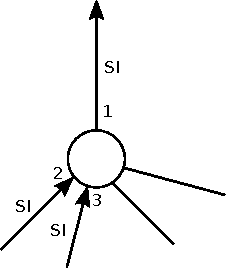
\includegraphics[scale=0.75]{images/n_32}
\end{center}

\theorem{
  L'algoritmo \texttt{DSP} costruisce uno ST del grafo e crea un orientamento locale compatibile con lo stesso, utilizzando $M[$\texttt{DSP}$/ RI] = 2m$. [Non fatto a lezione]
}

Si adatta a reti dinamiche:
\begin{itemize}
  \item se appare un arco nuovo, non lo consideriamo nell'esplorazione:
  \begin{center}
    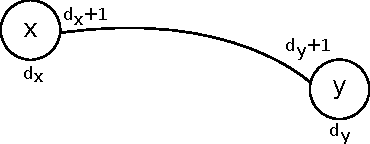
\includegraphics[scale=0.75]{images/n_33}
  \end{center}
  \item se appare un nuovo nodo con dei nuovi archi, scelgo un arco e metto \#porta 1 nell'arco che conduce al padre, mentre nel nodo raggiunto devo ``riaggiustare'' le numerazioni.
  \begin{center}
    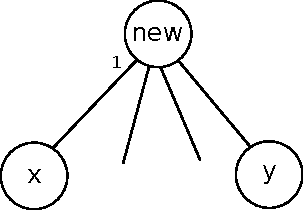
\includegraphics[scale=0.75]{images/n_34}
  \end{center}
  \item cancellazione di un arco non in ST: devo compattare i numeri di porta;
  \item cancellazione di un arco nello ST: devo sostituire integralmente lo ST;
  \item se cancelliamo un nodo di grado 1 (foglia nello ST) basta rinumerare:
  \begin{center}
    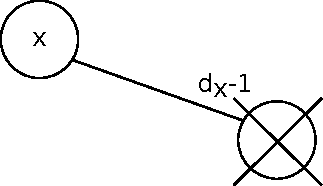
\includegraphics[scale=0.75]{images/n_35}
  \end{center}
  \item se cancelliamo un nodo di grado $> 1$, dobbiamo ricostruire lo ST.
\end{itemize}
\section{Miglioramento del Bound di 4n: Ci si basa sul numero di etichetta inserito}

Si può fare di meglio? Si!\\ \textbf{Facciamo in modo che all'etichetta più bassa corrisponde il sottoalbero più alto.}
In pratica l'automa avendo una "memoria" del passo precedente conosce la massima altezza che dovrà percorrere nell'arco successivo.
\textbf{Si ordinano le etichette di un generico nodo V in maniera inversamente proporzionale alla dimensione dei suoi sottoalberi.} Ovvero, più è piccola l'etichetta e maggiore sarà l'altezza del sotto albero. Le foglie quindi avranno tutte la stessa etichetta, quindi l'automa sbaglia nella prima o poi non sbaglia più. Questo funziona anche con le altre strutture della stessa altezza, dato che avranno lo stesso numero di porta, l'automa sbaglia una volta e poi finchè il numero di porta resta quello non sbaglia più.

\subsection{Descrizione delle strutture possibili}
Avendo questo ordinamento, la struttura più piccola che può stare nel sottoalbero è una foglia, che quindi avrà etichetta più grande di tutte le altre. Le foglie quindi avranno etichettamento consecutivo e quindi è possibile sbagliare nel primo arco, ma successivamente l'automa saprà che da li in poi saranno tutte foglie, e quindi non sbaglia più. Questo metodo si applica anche qualora ci fossero più strutture con la stessa etichetta, poichè potrò sempre risparmiare errori una volta aver sbagliato nella prima. Elenchiamone alcune:\\
Struttura prima di trovare una foglia: Un albero con altezza uno, ovvero due nodi messi a fila.\\
Ora abbiamo due possibilità:
\begin{itemize}
  \item Due nodi messi in fila
  \item Un nodo con due foglie.
\end{itemize}
Per ridurre il 4n dovrei eliminare un quantità di errori lineare rispetto al numero di nodi.
\subsection{Protocollo costruzione albero}

\begin{lstlisting}

Procedure Color(node v)
	node v become RED
	all nodes at distance 1 from v become GREEN
	all not yet colored nodes at distance 2 from v become BLUE
	
Procedure Backbone-Construnction(G) -> Tree
	pick an arbitrary node $v \in V$
	Color(v)
	$V_B = \{ v \}$ //nodi della backbone (all'inizio solo v)
	$E_B = \{ \emptyset \}$ //archi della backbone (all'inizio nessuno)
	while (the set of not colored nodes in $G \neq \emptyset$)
		pick a not colored node at distance 1 from some BLUE node $w_1$ 
			which is itself connected via node $w_2$ to some RED node v
		Color(v)
		$V_B = V_B \cup \{ w_1, w_2, v \}$
		$E_B = E_B \cup \{ (v',w_2), (w_2, w_1), (w_1, v)\}$
		node $w_1$ and $w_2$ becomes YELLOW
		
Procedure Tree-Construnction (G, B /*Backbone di G*/) -> ST
	$V_T = V_B$
	$E_T = E_B$
	
	[Stiamo estendendo la backbone in maniera tale da prendere i nodi a distanza 1 dai rossi. In termini di errori troviamo dei vantaggi poiche cosi
	facendo, i nodi rossi hanno il grado all'interno dell'albero uguale a quello che hanno nel grafo. Se il robot quindi si deve muovere da un nodo rosso non puo' sbagliare, dato che tutti gli archi di un nodo rosso sono tutti appartenenti allo ST che stiamo costruendo.]
	
	foreach node $v \in V\diagdown V_T$ at distance 1 from a RED node $v' \in V_B$ do
		$V_T = V_T \cup \{v\}$
		$E_T = E_T \cup \{(v,v')\}$
	foreach node $v \in V\diagdown V_T$ at distance 1 from some node $v' \in V_T$ do
		$V_T = V_T \cup \{v\}$
		$E_T = E_T \cup \{(v,v')\}$ 
		[Tutti i nodi che sono rimasti fuori dall'albero sono a distanza 1 da questo, e quindi li prendo]
    each YELLOW node v not connected to any BLUE made v' by edge $(v,v')\in E_T$ becomes ORANGE
\end{lstlisting}

\textbf{Osservazioni: }\\
\vspace{-10mm}
\begin{itemize}
\item I nodi rossi hanno tutti gli archi incidenti dentro lo ST.
\item Non è possibile che ci sia un nodo verde a distanza 1 da due nodi rossi.
\item Se prendiamo un qualunque nodo dell'albero che non sta nella backbone la sua distanza massima sarà 2, proprio per come è stato costruito
\item non si può comunque avere sottoalberi con altezza maggiore di 2
\end{itemize}

La Backbone è formata da nodi Rossi e Gialli con la proprietà che se il percorso che connette due nodi rossi contiene solo nodi gialli, allora ne contiene esattamente due di questi. I nodi rimanenti sono colorati o di Verde o di Blu se la loro distanza da un nodo rosso è 1 o 2 rispettivamente. La procedura ricolora tutti i nodi Gialli, che non hanno nodi Blu come vicini, in nodi Arancioni. Questa colorazione sarà utile per calcolare la lunghezza della distanza P.

Per andare ad etichettare il grafo dell'esempio sul quaderno le etichette 1 si mettono su tutti gli archi per andare VERSO la radice (dalle 4 regole viste all'inizio del paragrafo). I numeri di porta restanti vanno messi in base al numero di nodi nel sottoalbero e bisogna comunque numerare gli archi che non appartengono allo ST.

\textbf{Quanto risparmiamo con questo metodo?}\\
Se consideriamo un nodo rosso, esso avrà un certo numero di connessioni della backbone, se ora consideriamo il resto del vicinato e lo ordiniamo in ordine decrescente di size dei sottoalberi, più a destra possibile si avranno le foglie (gruppo L nel disegno), poi avremo le cosiddette foglie estese (gruppo E), poi i generici sottoalberi (gruppo A)

\begin{center}
    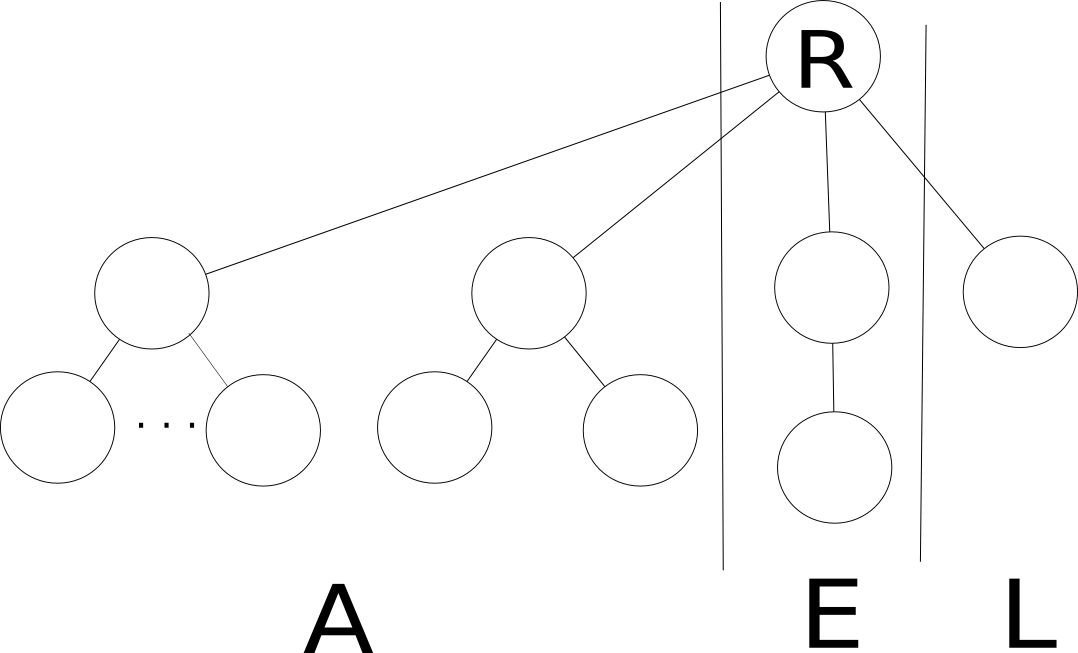
\includegraphics[scale=0.15]{images/automa1}
\end{center}

Consideriamo le tre tipologie in maniera separata, nel gruppo L l'automa farà al massimo un errore, nel gruppo E ne farà al massimo 2, uno nella foglia e uno nel nodo intermedio per controllare se ha un altro figlio, cioè se è ancora nel caso A, mentre per il tipo A saranno 2 errori per ogni tipo di sotto albero.\\ L'idea principale del protocollo è che inseriamo questi numeri di porta per fare in modo che \textbf{il robot esplori prima i sotto alberi più grandi e poi quelli più piccoli a mano a mano.}

v è un nodo rosso, indichiamo ad esempio $S_L(v)$ (numero di nodi di tipo L del nodo v) :
\begin{equation}\nonumber
S_L(v) = \begin{cases} 0, & \mbox{se il numero di figli di v di tipo L è 0}\\
1, & \mbox{altrimenti} \end{cases}
\end{equation}
\begin{equation}\nonumber
S_E(v) = \begin{cases} 0, & \mbox{se il numero di figli di v di tipo E è 0}\\
1, & \mbox{altrimenti} \end{cases}
\end{equation}
\begin{equation}\nonumber
S_A(v) = \#figliDiTipo A
\end{equation}

\begin{equation}
\begin{array}{ccc} 
S_L = \sum_{v \in RED} s_L(v) &
S_E = \sum_{v \in RED} s_E(v) &
S_A = \sum_{v \in RED} s_A(v) \\
S_Y = \#nodiGialli &
S_O = \#nodiArancioni &
S_R = \#nodiRossi
\end{array}
\end{equation}
Sia $n$ il numero di nodi e $p$ il numero di errori che possono commettere.\\
\textbf{Calcolo di n}\\
Avremmo:
$n \geq 3 S_A + 2 S_E + S_L + S_O + 2 S_Y + S_R$\\
Poichè 3 sono il numero di nodi che creano un sottoalbero di tipo A, 2 $S_e$ indica il numero di nodi se l'albero è una foglia estesa e 2 $S_y$ poichè i nodi gialli sono al più 2???
I nodi yellow che non sono diventati Orange è perchè hanno dei vicini Blue.\\
\textbf{Calcolo della Penalty [Vedere quaderno per i disegni su dove commetto errori]:} \\
Quanti errori commetto nella struttura $S_A$? Al più due.\\
Quanti errori commetto nella struttura $S_E$? Al più due.\\
Quanti errori commetto nelle foglie? Solo uno.\\
Quanti errori commetto sui nodi gialli? Al più due\\
Quanti errori commetto sui nodi Orange? Solo uno.\\
Quindi possiamo concludere che: la penalty è : \\
$p \leq 2 S_A + 2 S_E + S_L + S_O + 2 S_Y$\\
Mettiamoli in corrispondenza: \\
$p \leq 2 S_A + 2 S_E + S_L + S_O + 2 S_Y$\\
$n \geq 3 S_A + 2 S_E + S_L + S_O + 2 S_Y + S_R$\\

Sfruttiamo le seguenti proprietà per stimare il rapporto $p/n$\\
\vspace{-10mm}
\begin{itemize}
\item $S_Y + S_O = 2 S_R - 2$ Poichè $S_Y + S_O$ sono intermedi ai nodi rossi, se li sommo tutti ottengo due volte il numero dei rossi. (vedere quaderno per disegno)
\item $S_E \leq S_R$, $S_L \leq S_R$
\item $S_A \geq 0$
\end{itemize}
sommando sopra e sotto $S_O$ avremo: \\
$$\frac{2 S_A + 2 S_E + S_L + 2(S_Y + S_O)}{3 S_A + 2 S_E + S_L + 2(S_O + S_Y) + S_R} < \frac{2 S_A + 2 S_E + S_L + 4 S_R}{3 S_A + 2 S_E + S_L + 5 S_R} \leq \frac{2 S_A + 7 S_R}{3 S_A + 8 S_R} $$

Vediamo quindi il costo di questo algoritmo:\\
$$ 2n - 2 + 2p < 2n -2 + 2 \frac{7}{8} n = 3.75n -2 $$
Si ha 2P poichè commetto l'errore e torno indietro.\\
Risposta : SI, si può fare di meglio.\\

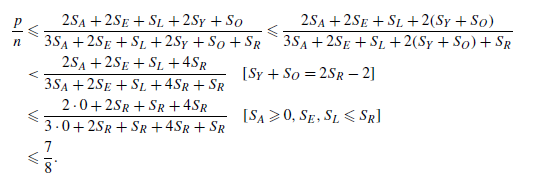
\includegraphics[]{images/66.png}\\
\textbf{Osservazione}: Senza stati, quindi senza memoria, il bound corrente è 4n-2.\\
$$O(2.8n) \leq Senza memoria (senza stati) \leq 4n-2$$
$$2n-2 \leq Con memoria \leq 3.5n -2 $$

Questo ultimo algoritmo fa riferimento a: \emph{Fast Periodic Graph Exploration with Constant Memory, 
L. Gasieniec, R. Klasing, R. Martin, A. Navarra, X. Zhang}


\chapter{Saturazione}\label{cap:saturazione}
In questa sezione, consideriamo i calcoli nelle reti ad albero sotto le restrizioni standard \textbf{R} più chiaramente, la conoscenza comune che la rete è un albero.\\
Si noti che la conoscenza di essere in un albero implica che ogni entità può determinare se è una \textbf{foglia} (cioè ha un solo vicino) o un nodo interno (cioè ha più di un vicino).\\
Abbiamo già visto come risolvere i problemi di Broadcast, Wake-Up e Traversal in una rete ad albero. I primi due sono risolti in modo ottimale dal protocollo Flooding, il secondo dal protocollo DF Traversal. Queste tecniche costituiscono il primo insieme di strumenti algoritmici per il calcolo in alberi con più iniziatori. Introdurremo ora un'altra tecnica molto basilare e utile, la \textbf{saturazione}, e mostreremo come può essere impiegata per risolvere in modo efficiente molti problemi diversi negli alberi indipendentemente dal numero di iniziatori e dalla loro posizione.\\
Prima di farlo, dobbiamo introdurre alcuni concetti e terminologia di base sugli alberi. In un albero T, la rimozione di un collegamento $(x,y)$ \textbf{disconnetterà T} in due alberi, uno contenente $x$ (ma non $y$), l'altro contenente $y$ (ma non $x$); li indicheremo rispettivamente con $T[x - y]$ e $T[y - x]$. Sia $d[x, y]$ = $Max\{d(x, z) : z \in T[y - x]\}$ la distanza maggiore tra $x$ e i nodi in $T[y - x]$. Ricordiamo che la distanza più lunga tra due nodi qualsiasi è chiamata \textbf{diametro} ed è indicata con $d$. Se $d[x, y] = d$, il cammino tra $x$ e $y$ si dice \textbf{diametrale}.

\section{Tecnica di Saturazione}
La tecnica della saturazione consiste nell'avere una configurazione iniziale (al tempo $t_0$) del nostro sistema in cui tutte le entità sono nello stato di Asleep (come nel Wake-up) ed avere una configurazione finale in cui il sistema avrà esattamente due entità nello stato di SATURATED e tutte le altre nello stato di PROCESSING. Per il funzionamento si assume come grafo un \textbf{albero T} non radicato e l'insieme delle restrizioni in cui si lavora è solo \textbf{R, si possono avere quindi più iniziatori.} Questa permetterà di trovare esattamente $2$ nodi vicini tra di loro e la tecnica consiste in tre stadi: %Permetterà di trovare esattamente $2$ iniziatori vicini tra loro ed assume come grafo un albero $T$ non radicato costruito sotto le restrizioni $R$.
\begin{enumerate}
  \item \textbf{Stadio di attivazione (Wake-Up)}: L'obiettivo è quello di eseguire il Wake-up. Viene svolto dagli iniziatori che, una volta diventati attivi, mandano un messaggio d'attivazione a tutti i loro vicini che diventeranno quindi Active. A loro volta attiveranno i loro vicini. Lo scopo è quello di avere tutti i nodi 'Active' (\texttt{Wake-Up}).
  \item \textbf{Stadio di saturazione (Convergecast)}: Viene iniziato dalle foglie dello ST. Queste inviano un messaggio $M$ al padre e passano allo stato di PROCESSING. Un nodo interno $x$ non appena riceve il messaggio $M$ da $deg(x) -1$ vicini, manda $M$ all'unico vicino che non gli ha mandato $M$ e considera questo come padre; inoltre passa allo stato di PROCESSING. Infine se un nodo nello stato di PROCESSING riceve $M$ da suo padre, passa allo stato di SATURATED. Lo scopo è quello di andare ad eleggere due nodi saturi (vedremo che sono due).
  \item \textbf{Stadio di risoluzione (Dipende)}:
  Viene iniziato dai 2 nodi saturati e la natura di questo stadio dipende dall'applicazione in cui ci troviamo.
\end{enumerate}
Ripetiamo come funziona lo stadio di saturazione:
\begin{itemize}
    \item Una foglia manda un messaggio M al proprio padre.
    \item Un entità non foglia aspetta di ricevere $|N(x)-1|$ messaggi di tipo M. Quando questo avviene manda M sull'unico link da cui non lo ha ricevuto.
\end{itemize}
Quindi si avranno: $\#msg(M) = n$, poiché ci sarà un arco in cui transitano due messaggi, la coppia di nodi di questo arco sarà la \textbf{coppia di nodi saturi}, viene infatti definita come tecnica \textbf{Edge-election}, perché è stato selezionato un arco.\\
\textbf{MIO:} Dato che si hanno n nodi e n-1 archi, trattandosi di un albero, ci sarà un singolo arco in cui vengono scambiati due messaggi M, i nodi che congiunge quell'arco saranno quelli SATURATED. Una volta che sono stati "scoperti" i nodi saturi inizia la fase di Risoluzione, che viene cominciata da quest'ultimi.\\
\theorem{
  Esattamente due nodi in stato di PROCESSING diventeranno SATURATED; inoltre questi 2 nodi sono l'uno il padre dell'altro (sono vicini).
 
%Per come abbiamo definito l'algoritmo, un'entità invia un messaggio M solamente a suo padre, e diventa SATURATED una volta che riceve M da quest'ultimo. Prendiamo ad esempio un nodo $x$ che invierà un messaggio M nel link che lo collega al suo parent. Prima o poi, dato che non sono presenti cicli, il messaggio arriverà ad un nodo SATURATED $s_1$. Questo nodo è diventato SATURATED perchè ha ricevuto un messaggio M dal suo parent $s_2$; poichè s2 ha inviato un messaggio M ad s1, s2 deve essere stato in PROCESSING e deve aver considerato s1 suo padre. Quindi quando il messaggio M di s1 arriverà su s2, anche s2 diventa saturo. Pertanto esistono almeno due nodi che diventano saturi.

\textbf{Dimostrazione}\\

  \begin{center}
    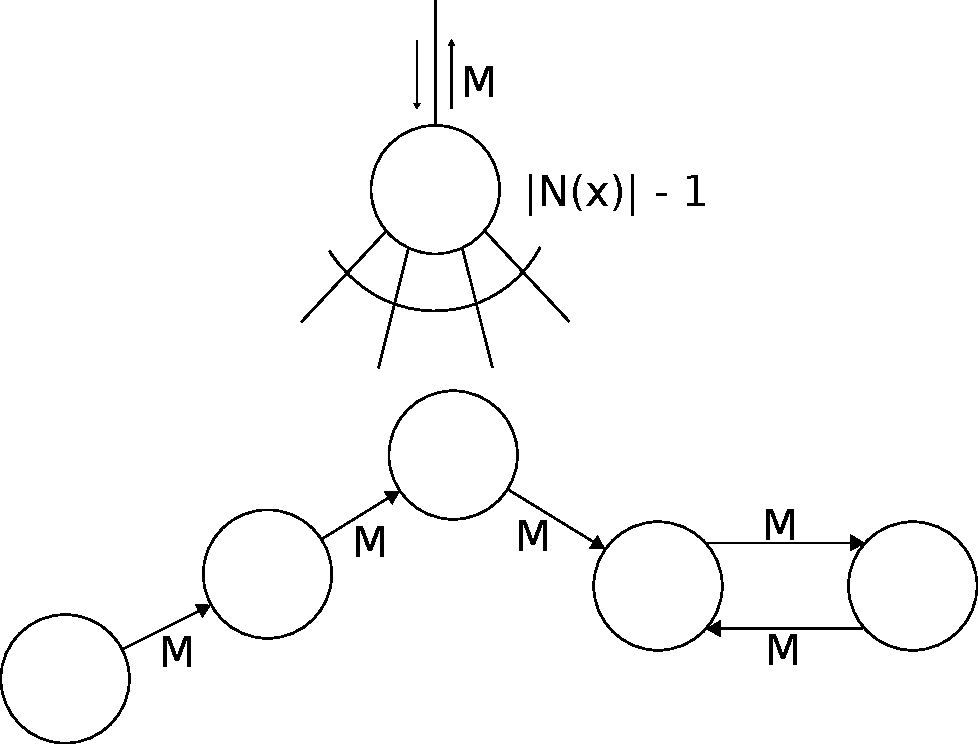
\includegraphics[scale=0.5]{images/n_40}
  \end{center}
\begin{itemize}
    \item \textbf{Dimostro che esattamente due nodi diventano Saturated:}
    \begin{enumerate}
        \item Supponiamo che $x$ nodo foglia invia un messaggio M a suo padre.
        \item Dato che ci troviamo su un albero non ci saranno cicli, quindi prima o poi questo messaggio raggiungerà un nodo $s_1$ in stato di SATURATED.
        \item 
        
        Questo nodo per essere diventato SATURATED deve aver ricevuto M da suo padre $s_2$, ma se $s_2$ ha inviato M allora è sicuramente in stato di PROCESSING e deve aver considerato $s_1$ suo padre.
        \item Quando M inviato da $x$ arriva ad $s_1$, questo lo invia a suo padre, che è $s_2$ ma questo è in stato di PROCESSING e riceve M, quindi diventa SATURATED.% tramite $s_1$ diventerà per forza anche lui SATURATED.
    \end{enumerate}
    
    
    %\\ Nel percorso fatto dai messaggi M, prima o poi arriviamo ad un nodo SATURATED poiché siamo in un albero (non abbiamo cicli). In particolare, quando arriviamo al nodo SATURATED, esso invia il messaggio M a suo padre, ma dato che è Saturated allora suo padre è sicuramente in stato di Processing, ovvero ha già inviato un messaggio M.
    %e quindi il nodo prima di lui avrà considerato il messaggio M, 
    Se me conclude che anche il nodo prima diventa SATURATED. Almeno due nodi diventano SATURATED.
    
    \textbf{Altra possibile dimostrazione:} Si può confermare che i nodi saturi sono 2 per la correttezza del Convergecast. Durante questo protocollo, ogni entità manda esattamente un messaggio, ma dato che le entità sono $n$ e gli archi in un albero sono $n-1$, ci sarà per forza un arco in cui transiteranno due messaggi M, e quell'arco è proprio quello che congiunge i due nodi saturi.
    
    
    \item \textbf{Dimostro che i nodi Saturated sono uno il padre dell'altro (sono vicini):}\\  Assumiamo, per assurdo, $\exists x,y$ SATURATED con la distanza tra di loro maggiore di 2.
  \begin{center}
    $d(x,y) \geq 2$

    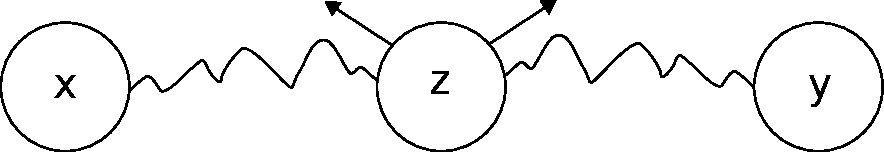
\includegraphics[scale=0.5]{images/n_41}
  \end{center}

In questo caso affinchè $x$ ed $y$ fossero nodi saturi $z$ dovrebbe aver mandato due messaggi di tipo M, ma questo è assurdo, perchè va contro le ipotesi del protocollo (non può esistere $z$ che manda due M nelle due direzioni: ogni nodo manda un solo M, questo è assurdo). Se ne conclude quindi che i due nodi saturi sono sicuramente vicini tra di loro.
  %Non può esistere $z$ che manda due M nelle due direzioni: ogni nodo manda un solo M, questo è assurdo. Contraddice che il nodo centrale dovrebbe inviare due messaggi M, la contraddizione è che tra X ed Y non ci deve essere nessuno se ci fosse, allora quel nodo dovrebbe aver mandato 2 messaggi Min in entrambe le direzioni

\end{itemize}
}

\textbf{Importante:} Quali nodi diventano saturi dipende strettamente dal ritardo di comunicazione e quindi è totalmente imprevedibile. Esecuzioni successive con gli stessi iniziatori potrebbero generare coppie di nodi saturi diverse ad ogni esecuzione.

\subsection{Complessità}
\underline{Messaggi [Prof]:}
$M[$\texttt{SatureTree,R,treee}$] \leq 2(n-1) + (n-1+1) = 3n - 2$
\begin{itemize}
    \item $2(n-1)$ è il costo della prima fase del Wake-Up
    \item $(n-1+1)$ è un singolo messaggio per arco, che in un albero sono $n-1$ mentre l'unico arco in cui transiteranno due messaggi è quello che connette i due nodi saturi, che quindi abbiamo un $+1$.
\end{itemize}
Supponiamo di avere $K^*$ iniziatori:
\begin{center}
  $M[$\texttt{SatureTree,R,treee}$] = n + K^* - 2 + (n-1+1) = 2n + K^* -2$\\
\end{center}
Dove:
\begin{itemize}
    \item $(n + K^* - 2)$ Costo del wake-up con $k^*$ iniziatori.
    \item $(n-1+1)$ uguale a sopra.
\end{itemize}

Durante il processo di saturazione, esattamente un messaggio viene trasmesso su ogni arco, tranne quello che connette i due nodi saturi, dove M viene inviato due volte, quindi il totale è $n-1+1 = n$ messaggi.


\underline{Tempo [Prof]:}
$T[$\texttt{SatureTree,R,tree}$] \leq d + d$
\begin{itemize}
    \item Il Primo d è il costo in tempo del Wake-up
    \item Il Secondo è del ConvergeCast (risalita del messaggio dalle foglie)
\end{itemize}
\underline{Tempo:}
Per determinare il tempo ideale siano:
\begin{itemize}
 \item $I \subseteq V$ iniziatori;
 \item $L \subseteq V$ foglie;
 \item $t(x)$ tempo dall'inizio dell'algoritmo fino a che $x$ non diventa ACTIVE.
\end{itemize}

Un nodo SATURED $s$ deve aspettare che tutte le foglie siano ACTIVE e che i messaggi M generati da esse lo raggiungano, quindi deve aver aspettato:
\begin{center}
  $\max \lbrace t(l) + d(l,s) : l \in L \rbrace$
\end{center}

Uno nodo non iniziatore $x$ diventerà ACTIVE al tempo:

\begin{center}
  $t(x) = \min \lbrace d(x,y) : y \in I \rbrace$
\end{center}

Quindi il costo totale è:

\begin{center}
  $T[$\texttt{FullSaturation}$] \leq \max \{ \min \{ d(l,y) \} + d(l,s) : y \in I, l \in L \} \leq 2d $
\end{center}

\textbf{ConvergeCast:}
\begin{enumerate}
    \item Una foglia invia un messaggio al parent.
    \item Ogni nodo interno aspetta fin quando non ha ricevuto tutti i messaggi dai suoi figli e successivamente invia un messaggio al proprio padre.
\end{enumerate}



\section{Esempio di applicazione: Protocollo MinFind}

$$P_{INIT} = < \forall x \in \xi, value(x) \in \mathbb{R}, status(x) = Avaiable>$$
$$
P_{FINAL} =   < 
  \forall x \in \xi, status(x)= MIN \; if \; value(x) = min
\{value(y), y \in \xi \}$$$$ \&\&  status(x) = LARGE \;altrimenti >$$
Vediamo ora un esempio di applicazione della Saturazione per trovare il più piccolo valore all'interno di un sistema. Ogni entità $x$ ha un certo valore $v(x)$ ed è in uno stato uguale a tutte le altre (AVAIABLE). L'obiettivo è quello di trovare il minimo tra tutti i valori $v(x)$ delle entità, e fare in modo che in terminazione ognuna di esse conosca se è o no il minimo all'interno del sistema, ed entrare rispettivamente nello stato di MINIMUM o LARGE.\\
\textbf{Attenzione:} L'insieme delle restrizioni sulle quali ci basiamo resta comunque $R$. Più di un'entità all'interno del sistema può avere il minimo valore poichè sono ammessi valori uguali tra più entità. Si assume un albero non radicato come grafo.\\
Si assume sempre rete ad Albero.
\begin{itemize}
    \item Se l'albero fosse radicato, allora il problema sarebbe più semplice, poichè in questa tipologia, è presente sia un nodo speciale (la radice) sia un orientamento logico dei link, infatti ogni nodo può capire quale link è "up", ovvero che lo porta alla radice, e quale link è "down", ovvero che lo allontana da quest'ultima. In questa tipologia, per trovare il minimo, la radice effettua un broadcast di richiesta "down" per richiedere la computazione del minimo valore dell'albero. Le entità poi effettueranno quello che è il convergecast iniziato dalle foglie. I nodo determineranno il minimo valore del proprio sotto albero e lo rispediranno nell'arco "up". Ne risulta che il minimo valore è computato alla radice, che effettuerà poi il broadcast di questo a tutti. \textbf{Il convergecast} può essere utilizzato solamente in un albero RADICATO.
    \item Nel nostro caso però non abbiamo un albero radicato, ma il processo di \textbf{Full Saturation} ci permette comunque di risolvere il problema della ricerca del minimo. Vediamo come funziona:
\end{itemize}

L'algoritmo inizia sempre con lo stadio di Attivazione, che farà in modo che tutte le entità siano ACTIVE. A questo punto quando inizia lo stadio di Saturazione, all'interno del messaggio M che parte dalle foglie, le entità inseriscono il valore minimo a loro conosciuto, quindi le foglie invieranno semplicemente il loro id, mentre un nodo interno terrà contro del minimo locale del suo sotto albero ed invierà a suo padre solamente questo. Ne segue che quando i due nodi saturi saranno eletti, sapranno il valore minimo del proprio sotto albero, che invieranno in broadcast nello stadio di Risoluzione.
%Nell'algoritmo tutte le entità partono dallo stato di Avaiable (che è lo stesso di ASLEEP), tramite impulso spontaneo un'entità inizia la propria esecuzione ed invia un messaggio a tutti i suoi vicini per fare in modo che tutte le entità, quando inizia lo stadio di Saturazione siano nello stato di ACTIVE. Un nodo diventa processing quando manda M al padre. Quando da processing ricevo altri M aggiorno il minimo locale.

%\textbf{Funzionamento dell'algoritmo:}
%Tramite il processo di saturazione vengono scambiati i minimi locali di ogni nodo includendo il valore che un'entità ha nel messaggio M, fino ad eleggere i due nodi SATURATED che avranno ognuno il minimo locale del proprio sotto albero. Questi due nodi si scambiano poi i due minimi venendo quindi a conoscenza del minimo globale. A questo punto inizia il processo di risoluzione (Stadio 3) dove viene fatto il \textbf{Broadcast} del messaggio di minimo su un albero partendo da due radici, quindi il costo è il seguente:

\underline{Messaggi:}\\
$M[$\texttt{MinFind,R,tree}$] \leq 3n - 2 + n - 2 = 4n - 4$
\begin{itemize}
    \item 3n - 2 è il costo della saturazione.
    \item n è il costo del broadcast.
    \item -2 sono i messaggi risparmiati sull'arco saturato, dove i nodi già conoscono il minimo globale.
\end{itemize}

\begin{center}
  $M[$\texttt{MINFIND,R,treee}$] = n + K^* - 2 + (n-1+1) + (n-2) = 3n + K^* - 4$\\
\end{center}
Dove:
\begin{itemize}
    \item $(n + K^* - 2)$ Costo del wake-up con $k^*$ iniziatori.
    \item $(n-1+1)$ uguale a sopra.
    \item $n-2$ costo del broadcast che viene avviato dai nodi saturi, risparmiamo due messaggi perchè i nodi saturi già conoscono il minimo globale.
\end{itemize}
Possiamo vedere che al costo della \textit{FullSaturation}, sono stati aggiunti $n-2$ messaggi utilizzati nel terzo stadio (\texttt{Broadcast} su albero partendo da due radici).


\underline{Tempo:}
$T[$\texttt{SatureTree,R,tree}$] \leq 3d$
\begin{itemize}
    \item d nel sottografo del primo nodo saturato
    \item d nel sottografo del secondo nodo saturato
    \item d Broadcast del messaggio
\end{itemize}


Il costo di T ed M è ottimo asintoticamente, poichè è obbligatorio che tutti i nodi del grafo siano presi in considerazione [Vedere quaderno di Carpi, in fondo, per disegni].\\
\underline{Tempo [Studenti]:}
\begin{center}
  $T[$\texttt{TreeElectMin}$] = T[$\texttt{FullSaturation}$] + \max \{ d(s, x) : s \in S, x \in V \} \leq 3d$
\end{center}

Tramite saturazione possiamo risolvere anche: massimo, somma elementi, prodotto, predicati logici; in pratica tutte le funzioni dette di semigruppo, in cui valgono le proprietà commutativa e associativa. Si possono fare anche alcune funzioni statistiche tipo la media. In particolare vedremo di seguito come la ricerca dell'eccentricità tramite saturazione faccia scendere il costo da $n^2$ a $n$.

\section{Ricerca dell'eccentricità}
La tecnica di base è stata finora utilizzata per risolvere problemi a valore singolo; cioè problemi la cui soluzione richiede l'identificazione di un unico valore. Può anche essere utilizzato per risolvere problemi multivalore come il problema di determinare le \textbf{eccentricità} di tutti i nodi.\\
Utilizziamo adesso la Saturazione per trovare l'eccentricità dei nodi saturi all'interno dell'albero. Iniziamo con una definizione:\\
\definition{
L'eccentricità di un nodo $x$, denotata con $r(x)$, è la più grande distanza tra $x$ e ogni altro nodo nell'albero: $$r(x) = Max\{d(x,y) : y \in V)\}$$
Notiamo che il \textbf{centro} è il nodo con eccentricità minima.
}\\
\definition{
In un albero, dato un arco $\{x,y\}$ si denota con $T[x - y]$ l'albero contenente $x$ ma non $y$ ottenuto rimuovendo l'arco $\{x,y\}$
}

Applicando la definizione appena descritta si ottengono quindi 2 sottoalberi, uno che contiene il nodo $x$ che sarà $T[x - y]$, l'altro invece conterrà il nodo $y$ e sarà $T[y - x]$. \\\\
\textbf{Come si calcola l'eccentricità di un singolo nodo:}\\
Per calcolare la propria eccentricità, un nodo $x$ deve determinare la massima distanza da tutti gli altri nodi. Per far questo, $x$ deve effettuare il Broadcasting della richiesta, diventando automaticamente lui la radice dell'albero, si utilizza poi il convergecast sull'albero radicato in $x$; facendo questo si colleziona la massima distanza dagli altri nodi.\\
\textbf{Costo messaggi:} $2(n-1)$ dove:
\begin{itemize}
    \item n-1 è  per il Broadcast
    \item n-1 è per il Convergecast
\end{itemize}
Se volessi utilizzare questo metodo per il calcolo dell'eccentricità di ogni nodo, si spenderebbe $n(2(n-1))$ poichè ogni nodo effettua un numero di messaggi pari a $2(n-1)$.\\

\textbf{Il costo per il calcolo dell'eccentricità di ogni nodo con il metodo precedentemente descritto è O($n^2$). Mostreremo adesso che tramite la saturazione il costo scende a O($n$)}\\

\textbf{Possiamo usare la saturazione per rilevare l'eccentricità di tutti i nodi aggiungendo al messaggio M un valore di "altezza".}

\subsection{Calcolo dell'eccentricità di ogni nodo tramite Saturazione: Protocollo Eccentricity}
Il nostro obiettivo è quello di determinare l'eccentricità di ogni nodo. Il primo passo per la risoluzione del problema consiste nell'applicare la Saturazione per calcolare l'eccentricità dei due nodi saturi. Da notare che non sappiamo a propri quali nodi diventeranno saturi, ma basta sapere che quando ci diventano sapranno sicuramente la loro eccentricità. Per far questo è necessario includere nel messaggio M inviato da un'entità $x$ al parent $y$ la \textbf{massima} distanza di $x$ dai nodi del suo sotto albero $T[x-y]$ (che non contiene y)+ 1, poichè deve arrivare ad $y$. In questo modo un nodo saturo $s$ saprà la distanza $d[s,y]$ per ogni vicino $y$; quindi potrà calcolare la sua eccentricità. \\
Il nostro obiettivo però è calcolare l'eccentricità di ogni nodo, non solo quella dei nodi saturi.\\

La cosa interessante è che le informazioni disponibili presso ciascuna entità al termine della fase di saturazione sono quasi sufficienti per farle calcolare la propria eccentricità.\\
Consideriamo un'entità $u$; ha inviato il messaggio $M$ al suo genitore $v$, dopo averne ricevuto uno da tutti gli altri suoi vicini; il messaggio da $y \neq v$ conteneva $d[u, y]$. In altre parole, $u$ conosce già la distanza massima da tutte le entità \textbf{tranne} quelle nell'albero $T[v - u]$. Pertanto, l'unica informazione che manca a $u$ è $d[u, v] = Max\{d(u, y) : y \in T[v - u]\}$. Notare che 
$$
d[u, v] = Max\{d(u, y) : y \in T [v - u]\} = 1 + Max\{d[v, z] : z \neq u \in N (v)\}.
$$
Riassumendo, ogni nodo, tranne quelli saturi, \textbf{manca di un'informazione: la distanza massima dai nodi dall'altra parte del collegamento che lo collega al suo genitore}. Se i genitori possono fornire queste informazioni, l'attività può essere completata. Sfortunatamente, anche ai genitori mancano le informazioni, a meno che non siano i nodi saturi.\\
I nodi saturi hanno tutte le informazioni di cui hanno bisogno. Hanno anche le informazioni che mancano ai loro vicini: sia $s$ un nodo saturo e $x$ sia un vicino insaturo; a $x$ mancano le informazioni $d[x, s]$; per l'equazione sopra, questo è esattamente $d[x, s] = 1 + Max\{d[s, z] : x \neq z \in N(s)\}$, e $s$ conosce tutti i $d[s, z]$ (erano inclusi nei messaggi $M$ ricevuti). Quindi, i nodi saturi $s$ possono fornire le informazioni necessarie ai loro vicini, che possono quindi calcolare la loro eccentricità. La buona proprietà è che ora questi vicini hanno le informazioni richieste dai propri vicini (più lontani dai nodi saturi). Pertanto, la fase di risoluzione di \textit{Full Saturation} può essere utilizzata per fornire le informazioni mancanti: partendo dai nodi saturati, una volta che un'entità riceve le informazioni mancanti da un vicino, calcolerà la sua eccentricità e fornirà le informazioni mancanti a tutti gli altri suoi vicini.\\

\textbf{ATTENZIONE:} Nello stadio di Risoluzione l'informazione che viene propagata non è una notifica, poichè è diversa per ogni vicino che la riceve, ma resta comunque un singolo messaggio.

Gli algoritmi utilizzati nelle tre fasi quindi sono:
\begin{itemize}
    \item Wake-up
    \item Saturazione
    \item Broadcast NON di notifica, ogni entità riceve un informazione diversa.
\end{itemize}
\textbf{Costo dei Messaggi:}
\begin{itemize}
    \item $2n-2$ per il Wake-Up
    \item $n$ per la saturazione
    \item $n-2$ nella fase di risoluzione (Broadcast)
\end{itemize}
Si avranno quindi $4n-4$ messaggi (esattamente come il MinFind).

\textbf{Costo del Tempo:}\\
Paghiamo $d$ per tutte e 3 le fasi, quindi si avrà $3d$.

\section{Calcolo del Centro dell'albero}
Il centro in un grafo/albero è il nodo con eccentricità minore, ovvero il nodo che ha la distanza minima da ogni altro nodo all'interno del grafo. Da notare che una rete può avere più di un centro. Risolvere questo problema implica fare in modo che ogni entità in fase di terminazione entri rispettivamente nello stato di $center$ o $notCenter$.\\
\subsection{Sviluppo del protocollo}
Per risolvere il problema del Centro possiamo utilizzare il fatto che il centro è l'entità che ha eccentricità minima. Applicheremo quindi:
\begin{enumerate}
    \item Protocollo Eccentricity per trovare l'eccentricità di ogni nodo. Questa parte sarà iniziata dagli iniziatori.
    \item Ultime due fasi del MinFind. Questa parte sarà iniziata dalle foglie che tramite il Convergecast potranno inviare M al loro padre che conterrà il loro valore di eccentricità.
\end{enumerate}
Infine i saturi invieranno in broadcast il minimo trovato in modo che tutti i nodi lo conoscano e quindi un'entità può determinare se è centro o meno, cambiando stato rispettivamente in $center$ oppure $notCenter$.

\textbf{Messaggi:}
\begin{itemize}
    \item $4n - 4$ per l'eccentricity.
    \item $n$ fase risalita della ricerca del minimo (ConvergeCast).
    \item $n-2$ Broadcast finale.
$$Totale: 6n -6$$
\end{itemize}
\textbf{Tempo:}
\begin{itemize}
    \item $3d$ per Eccentricity.
    \item $d$ per ConvergeCast.
    \item $d$ per il Broadcast.
    $$Totale: 5d$$
\end{itemize}

\subsection{Miglioramento del protocollo di ricerca del Centro}
Possiamo migliorare il protocollo grazie a delle proprietà relative ai centri in un albero. Siano $d_1[x]$ e $d_2[x]$ il valore più grande ed il secondo valore più grande tra tutti i valori ricevuti da x durante l'applicazione del protocollo di ricerca dell'eccentricità, cioè tra la massima distanza tra $x$ ed i nodi del sotto albero $T[y-x]$ (\textbf{Attenzione: Quindi la massima distanza tra $x$ e L'ALTRO sotto albero NON radicato in lui}) per ogni $y$ vicini ad $x$. In simboli: 
\begin{center}
    $d_1[x]$ e $d_2[x]$ sono il valore più grande ed il secondo valore più grande in $T[y-x]$ 
\end{center}
Il centro di un albero ha interessanti proprietà tra le quali:\\
\lemma[2.6.2]{
In un albero o c'è un unico centro o ce ne sono 2 e sono vicini tra loro.
}\\
\textbf{Dim:} Supponiamo per assurdo che  esistono due centri $x$ ed $y$ non vicini tra loro e sia $p$ il cammino che connette $x$ ad $y$. Visto che abbiamo supposto $x$ ed $y$ non vicini allora il cammino $p$ conterrà almeno un altro nodo, ma può anche contenere altri sotto alberi radicati in questo nodo.\\
Il nodo più lontano da $x$ (che quindi ne determina l'eccentricità) può essere:
\begin{itemize}
    \item o in un sotto albero di $x$: Se così fosse $y$ sarebbe comunque più lontano e allora sarebbe solo $x$ il centro.
    \item o in un sotto albero di $y$: Se così fosse $x$ sarebbe comunque più lontano e allora sarebbe solo $y$ il centro.
    \item o in un sotto albero di $p$: Se così fosse dovrebbe esistere un centro sul Path ma anche questo è assurdo.
\end{itemize}
Se ne conclude che non può esistere un cammino tra i due centri.

\lemma{In un albero tutti i centri giacciono su tutti i percorsi diametrali.}

\lemma[2.6.3]{
Un nodo $x$ è centro se e solo se $d_1[x]-d_2[x]\leq 1$, inoltre se vale la disuguaglianza stretta allora $x$ è l'unico centro.\\
}

\textbf{Dim:}
Supponiamo $x$ sia l'unico centro e:
\begin{itemize}
    \item Se $d_1[x]-d_2[x] > 1$: Se così fosse, il nodo $y$ che determina $d_1[x]$ avrebbe distanza minore di $x$ da tutti gli altri e perciò sarebbe lui il centro. Ma questo è assurdo perchè $x$ è centro per supposizione.
    \item Se $d_1[x]-d_2[x] = 1$: Allora anche il nodo $y$ che determina $d_1[x]$ sarà un centro perchè avrà le stesse distanze di $x$ dagli altri nodi. Ma per supposizione $x$ era l'unico centro.
    \item Se $d_1[x]-d_2[x] = 0$: Il lemma vale, perchè $x$ è l'unico centro, qualunque altro nodo diverso da $x$ andassi a scegliere sarebbe più lontano da tutti gli altri nodi.
\end{itemize}

\lemma{Siano $y$ e $z$ vicini di $x$ tali che $d_1[x] = d[x, y]$ e $d_2 [x] = d[x, z]$. Se $d[x, y] - d[x, z] > 1$, allora tutti i centri sono in $T [y - x]$.}

Il lemma 2.6.3 ci da le informazioni necessarie per cambiare il protocollo sopra descritto. Un'entità $x$ può determinare se è o no $centro$ se viene a conoscenza del valore $d[x,y]$ di ogni suo vicino $y$. Ma questa informazione è esattamente quella che viene data ad un entità dall'applicazione del protocollo Eccentricity. Questo comporta che per risolvere il problema del centro è necessario solamente il suddetto protocollo. Quando un'entità ha l'informazione necessaria a computare il suo raggio, controllerà se il più grande valore ed il secondo più grande valore che ha ricevuto differiscono di almeno uno. Se così fosse allora diventerà $centro$, altrimenti cambierà stato in $notCenter$\\
\textbf{Calcolo del Costo:}
Nel protocollo precedentemente descritto si utilizza solamente l'Eccentricity e qualche calcolo addizionale, ma comunque il costo resta il medesimo di quest'ultimo protocollo.
\begin{itemize}
    \item Messaggi: $4n - 4$
    \item Tempo: $3d$
\end{itemize}

\chapter{Leader Election}
Il problema della Leader Election consiste nell'avere una configurazione iniziale del sistema in cui tutte le entità partono dallo stesso stato (AVAIABLE) e concludere con una configurazione avente tutte le entità nello stato di FOLLOWER tranne una che sarà nello stato di LEADER.
%Qualche volta è necessario che una determinata entità in un ambiente distribuito diventi temporaneamente il controller centrale di tutto il sistema. Per far questo, esistono protocolli che fanno in modo che tutte le entità partono da uno stesso stato AVAIABLE e al termine del protocollo tutte le entità saranno nello stato di FOLLOWER ed uno solo è nello stato di LEADER.\\
LEADER può diventarci qualsiasi entità, poichè non sono presenti restrizioni sul quale entità deve diventare leader oppure quante entità iniziano la computazione.
$$P_{INIT}=< \forall x \in \xi, status(x)=AVAILABLE >$$
$$P_{FINAL}=< \exists x \in \xi, status(x)=LEADER \text{ \& } \forall y \neq x \text{ , } status(y)=FOLLOWER >$$
La scelta del Leader può essere vista come un modo per ``forzare'' l'iniziatore unico in tutti i protocolli visti.
Esiste, tuttavia, un risultato di \textbf{impossibilità} sotto R (link bidirezionali, connettività, e affidabilità totale), ovvero che non esiste un protocollo deterministico che termina sempre correttamente in tempo finito se le restrizioni sono solo quelle di R:\\
\theorem{
  Il problema della Leader Election è deterministicamente non risolvibile sotto R.
\begin{proof}
 Basta considerare una rete costituita da 2 sole entità identiche, con gli stessi numeri di porta e con lo stesso stato (stesso valore iniziale).
 
 \begin{center}
  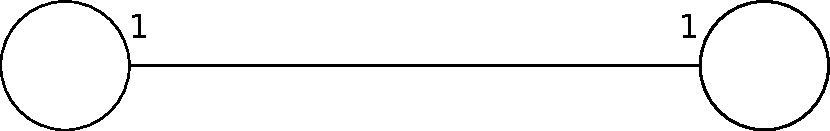
\includegraphics[scale=0.3]{images/n_42}
 \end{center}
 Sia P un protocollo che risolve il problema della Leader Election sotto R, questo protocollo deve risolvere il problema sotto qualsiasi circostanza. Consideriamo uno scenario in cui le due entità iniziano il protocollo P simultaneamente e abbiamo un ritardo di comunicazione unitario. Le due entità essendo identiche avranno la stessa esecuzione, se una riceve il messaggio anche l'altra lo riceverà e così via, se una diventa Leader anche l'altra diventa Leader, ma questo va contro la richiesta, ovvero quella che ci deve essere un solo leader, quindi P non è un protocollo che risolve il problema.
\end{proof}
}
La conseguenza di questo teorema è che bisogna rompere la simmetria, ma sotto R questa simmetria non si riesce a rompere. Il primo approccio sarebbe quello di aggiungere la restrizione di Inizializzatore Unico, ma in questo caso avremmo già il leader, e quindi sarebbe inutile applicare il protocollo. Dobbiamo quindi scartare questa possibilità e modificare le restrizioni in modo tale da ``distinguere'' ogni entità. Per far questo è comune utilizzare una specifica restrizione, che riguarda l'assegnamento di valori distinti (id) ad ogni entità. Chiamaremo questo nuovo s et di restizioni: Insieme standard per l'elezione:

\definition{
  Si dice \textbf{insieme standard per l'elezione}, l'insieme di restrizioni
  \begin{center}
    $IR = R \cup {ID}$
  \end{center}
}

\section{Elezione del Leader}
Come possiamo utilizzare questa nuova restrizione per rompere la simmetria ed eleggere quindi un leader?
Analizzando il problema della Leader Election, non importa quale delle entità diventi Leader, basta che ce ne è una, quindi utilizzando il fatto che i valori iniziali sono distinti per ogni entità, una possibile soluzione potrebbe essere quella di scegliere l'entità con il valore minore:
\begin{itemize}
 \item \texttt{Elect Minimum}
 \begin{enumerate}
    \item Trova il valore più piccolo;
    \item Eleggi come LEADER l'entità con tale valore.
  \end{enumerate}
Altro approccio:
  \item \texttt{Elect Minimum Initiator}
 \begin{enumerate}
    \item Trova il valore più piccolo tra gli iniziatori;
    \item Elegge come LEADER l'entità con tale valore.
  \end{enumerate}
Altro approccio ancora potrebbe essere quello di utilizzare i valori distinti delle entità per costruire uno spanning tree della rete ed eleggere la radice come nodo Leader:
  \item \texttt{Elect Root}
  \begin{enumerate}
    \item Costruisce uno ST radicato;
    \item Elegge come LEADER la radice.
  \end{enumerate}
\end{itemize}

Entrambi i protocolli funzionano \underline{solo} sotto le restrizioni IR, quindi da qui in avanti prendermo questo determinato set di restizioni. Il problema della leader election dipende dal sistema su cui si stiamo basando.

\section{Election su alberi: utilizzo del protocollo Saturation}
Supponiamo di lavorare su una topologia ad albero, quindi dove $m = n-1$:

\begin{itemize}
  \item Elezione con \texttt{Elect Min}\\
  Abbiamo già visto come trovare in modo ottimale il valore minimo di un albero utilizzando la \textbf{Saturazione.} Il protocollo che abbiamo studiato si chiama \textbf{MinFind}, supponendo che abbiamo ($K^*$) iniziatori il costo della leaderElection tramite questo metodo è:
  \begin{center}
    $M[$\texttt{TreeElectMin}$] = (2n + K^* -2) + (n-2) = 3n + K^* - 4 \leq 4n - 4$
  \end{center}
  dove: 
\begin{itemize}
    \item $(2n + K^* -2)$ è il costo della saturazione con $K^*$ iniziatori.
    \item $(n-2)$ è il costo del broadcast per comunicare alla rete chi è il Leader.
\end{itemize}
  
  La strategia di Elect Minimum Initiator ha lo stesso costo di questo approccio.
  \item Elezione con \texttt{Elect Root}\\
  Usiamo i primi due stage della Saturazione per eleggere i due nodi saturati, poi questi due si scambiano il loro ID ed il minimo diventa LEADER:
  \begin{center}
    $M[$\texttt{TreeElectRoot}$] = (2n + K^* -2) +2 + (n-2) = 3n + k^* - 2 \leq 4n - 2$
  \end{center}
\end{itemize}
\begin{itemize}
    \item $(2n + K^* -2)$ Costo normale della Saturazione con $K^*$ iniziatori.
    \item $+2$ Sono i due messaggi che si scambiano i nodi saturi per capire chi di loro è il minimo
    \item $n-2$ Notifica in broadcast
\end{itemize}


Dei due metodi è preferibile il secondo se consideriamo la lunghezza in bit dei messaggi:

In questo approccio solo n messaggi nella Saturazione portano un valore, mentre tutti gli altri solo segnali. Quindi il numero totale di bit trasmessi sarà:
\begin{center}
  $B[$\texttt{TreeElectMin}$] = n (c + \log_2 id) + c (2n + k^* - 2) = O(n \log n + n) = O(n \log n)$\\
%Dove id denota il valore maggiore inviato in un messaggio e c = O(1) denota il numero di bit richiesti per distinguere tra differenti messaggi. 
  $B[$\texttt{TreeElectRoot}$] = 2(c + \log_2 id) + c(3n + k^* - 2) = O(\log n + n) = O(n)$
\end{center}
Nell'elezione tramite la radice, solamente il messaggio di Election porta un ID di un nodo.
Dove:
\begin{itemize}
  \item $c$: bit per rappresentare i segnali (O(1));
  \item $id$: ID più grande da inviare in un messaggio.
\end{itemize}
Quindi in termini di numero di bit, Elect Root è migliore di Elect Minimum.
\section{Election su ring}
Un ring consiste in un ciclo di lunghezza n, dove ogni entità possiede esattamente due vicini; a livello topologico c'è una totale simmetria delle entità.\\ 
L'etichettamento \underline{non} è ordinato (è arbitrario) quindi globalmente le entità \underline{non} hanno la stessa destra e sinistra ma localmente distinguono le due direzioni.
\begin{center}
  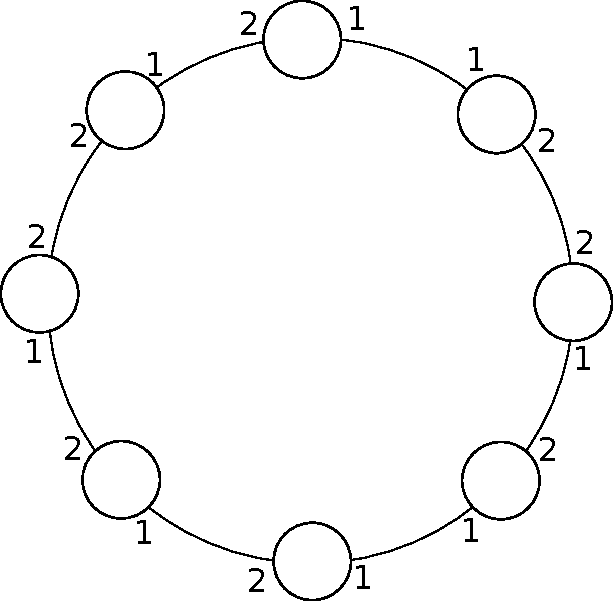
\includegraphics[scale=0.5]{images/n_43}
\end{center}
Consideriamo adesso il problema della Leader Election in un ring chiamato R sotto le restrizioni IR \{\textit{Bidirectional Links, Connectivity, Total Reliability, Initial Distinct Values}\}, ovvero ogni entità ha un valore iniziale diverso dalle altre.\\ Analizziamo il problema di trovare il minimo e di eleggere un nodo all'interno di un ring. Chiameremo gli "altri" gli $N(x) - $ sender di un'entità $x$.

\subsection{All The Way: Risoluzione del problema della Leader Election su Ring}
Stati del protocollo:
\begin{itemize}
    \item Asleep, Awake, Follower, Leader
    \item $S_{init}$ = ASLEEP
    \item $S_{term}$ = FOLLOWER, LEADER
\end{itemize}
Quando un'entità inizia, sceglie uno dei due vicini e gli invia un messaggio di "Election" contenente il suo id; quando un'entità riceve l'id di un altro nodo propaga il suo e quello che gli è arrivato, tenendo traccia dell'id minimo visto fino ad ora. Ogni messaggio viaggia fin quando non torna dall'entità che lo ha spedito.\\
\textbf{Terminazione:} Per la terminazione si utilizza un contatore per ogni entità, per tenere traccia di quanti ID diversi vengono ricevuti, ed un contatore in ciascun messaggio, in modo che ciascuna entità possa determinare $n$ quando riceve il suo messaggio dalla parte opposta da quella in cui l'ha spedito. Quando un'entità ha ricevuto un messaggio da tutte le altre $n$ (ed è a questo che serve il contatore) sà che ha terminato il protocollo e se ha ID pari al minimo cambia stato in LEADER. Se un'entità ha l'id maggiore del minimo, cambia stato in FOLLOWER.\\
\textbf{Attenzione:} In questo protocollo non è presente la notifica finale, un'entità una volta che capisce quante altre entità stanno partecipando al protocollo (è il valore $n$) saprà se ha ricevuto il messaggio da tutte le altre. Finchè questo non accade non può terminare la sua esecuzione. Quando invece ha ricevuto un messaggio da tutte le altre può cambiare stato o in LEADER o in FOLLOWER in base al suo id.

\textbf{Calcolo del costo:}\\ \textbf{Un messaggio originato da ciascuna entità viaggerà attraverso tutto il ring esattamente una volta.} Quindi si avranno esattamente $n^2$ messaggi in totale, ognuno contenente un contatore e un valore per un totale di $n^2log(id+n)$ bits, per quanto riguarda il tempo invece si avrà al più 2n. \textbf{Il caso pessimo è quando c'è un unico iniziatore.}\\
\underline{Messaggi:}
\begin{center}
  $M[$\texttt{AllTheWay}$] = n^2$ (è effettivamente =)
\end{center}
\underline{bit:}
\begin{center}
  $B[$\texttt{AllTheWay}$] = n^2*\log_2(id+n)$
\end{center}

Perchè ognuno degli $n^2$ messaggi contiene un contatore ed un id. Il contatore al massimo arriverà ad $n$.

%poiché codifichiamo insieme $id$ (al massimo $n$) e $cont$ (al massimo è $n$).

\underline{Tempo:}
\begin{center}
  $T[$\texttt{AllTheWay}$] \leq (n - 1) + n   = 2n - 1$
\end{center}
\begin{itemize}
    \item (n-1) indica il dover passare tutte le entità meno una per svegliare il minimo qualora non fosse già sveglio (caso peggiore).
    \item n invece sono i messaggi inviati dal minimo quando si sveglia.
\end{itemize}



\begin{center}
  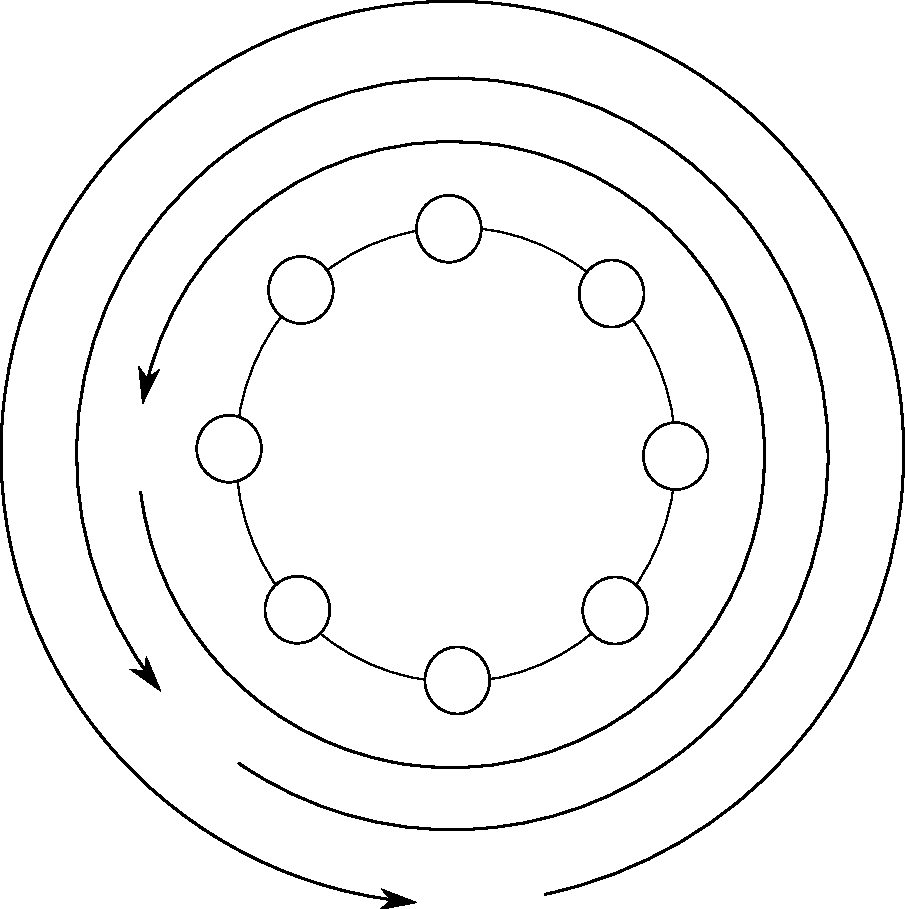
\includegraphics[scale=0.5]{images/n_44}
\end{center}

\textbf{Risoluzione dell'Elect Minimum Initiator tramite All The Way:} Si deve trovare il valore minimo tra tutti gli initiator. In questo caso tutte le \textbf{altre} entità non invieranno nessun messaggio, ma si limiteranno a propagare solamente il messaggio contenente l'id più piccolo che hanno ricevuto, non originando quindi nessun messaggio. Bisogna stare attenti però, perchè va modificata la parte del contatore, in quanto non tutte le entità che propagano possono essere iniziatori. Quindi si ha un problema sulla terminazione. Per come abbiamo definito il protocollo però, solamente l'effettiva entità che ha $id$ più piccolo riceve un messaggio con il suo stesso $id$ dall'altra parte in cui ha effettuato la send, quindi questa potrà poi notificare a tutte che il protocollo può terminare. Questo avviene tramite il messaggio di notifica da parte del LEADER che farà cambiare stato a tutte le altre entità che partecipano al protocollo in FOLLOWER.\\
\underline{Messaggi:}
\begin{center}
  $M[$\texttt{AllTheWayMINIT}$] \leq nk^* + n $
\end{center}
\underline{Tempo:}
\begin{center}
  $T[$\texttt{AllTheWayMINIT}$] \leq 3n - 1$
\end{center}
Quindi, qualora ci fosse un unico inizializzatore in questo caso si risparmiano molti messaggi, ed è il best case che è $O(n)$. Se invece tutte le entità sono inizializzatori questo protocollo utilizza $n$ messaggi in più dell'altro metodo.

\subsection{As far as it can}\label{asfar}
Il protocollo inizia con tutte le entità in stato di AVAIABLE. Queste, quando ricevono un impulso spontaneo inviano tutte nella stessa direzione il loro messaggio di election che contiene il loro $id$ e cambiano stato in AWAKE. Un'entità in stato di AVAIABLE riceve il messaggio di election invia il suo messaggio e controlla se ripropagare anche quello che gli è arrivato.
Se un'entità riceve un ID più grande di quello che ha visto fino ad adesso non effettua il forwarding di tale messaggio. Tutti gli iniziatori che iniziano tramite impulso spontaneo scelgono la stessa direzione nella quale inviare i messaggi, in questo caso \textbf{right}. Se un'entità è in stato di AVAIABLE = ASLEEP riceve un messaggio di Election allora:
\begin{itemize}
    \item Invia il suo messaggio contenente il suo id all'interno della rete e SUCCESSIVAMENTE controlla se ripropagare o no il messaggio che gli è appena arrivato.
    \item Per la decisione, controlla se  il valore di tale messaggio è minore del minore id che ha visto fino ad adesso. Se così fosse allora effettua il forwarding di tale messaggio (generando quindi un nuovo messaggio).
    \item Un'entità in stato di AWAKE, genera messaggi SOLAMENTE se hanno un valore più piccolo di tutti quelli visti fino a quel momento.
\end{itemize}
\textbf{Terminazione:} Siamo sicuri che il protocollo termina poichè solo il messaggio con ID minimo finisce il giro e solo l'entità con quell'ID saprà di essere il leader. A questo punto l'unica entità a conoscenza del fatto che il protocollo può terminare lo comunica agli altri con un singolo messaggio di notifica ed il protocollo termina essendo eletto il LEADER.

\textbf{Quando un'entità termina la propria esecuzione?}\\
Il messaggio avente id minimo attraverserà sempre tutto il ring, perchè nessuna entità lo fermerà, e quindi sarà l'unico che ritorna al suo mittente. Questo fatto ci da la possibilità di costruire un meccanismo per far terminare il protocollo. Se un'entità riceve un messaggio con il suo stesso id, allora sa di essere il minimo, e quindi il LEADER. Tutte le altre entità avranno visto questo messaggio, ma non sapranno se potrebbero arrivare altri messaggi contenenti id più piccoli di quello visto da loro. Quindi per assicurare la terminazione, il leader invia la notifica in una direzione del link, che attraverserà tutte le altre entità facendo cambiare stato in FOLLOWER.\\
\underline{Messaggi:}

\begin{center}
    Il LowerBound dei messaggi per la Leader Election è $\Omega(nlogn)$ su sistemi Asincroni
\end{center}{}

Ovviamente questo protocollo ha un numero di messaggi minore uguale di quello precedente, il numero esatto dipende da molti fattori. Considerando il costo del messaggio di "Election", esso attraverserà il ring fino a quando non trova un'entità avente id minore oppure completerà il giro. Quindi il costo dipende da come sono posti gli id all'interno del ring.\\
\textit{Worst Case:} L'id \#1 si sveglia prima di tutti ed invia il messaggio verso l'entita con id 2. Esso attraverserà sempre tutto il ring, costando n messaggi. L'id \#2 si fermerà solamente all'entità con id \#1, quindi il costo nel worst case è $n-1$, ottenibile se l'id \#2 è collocato immediatamente dopo l'id \#1 nella stessa direzione. In generale quindi l'id \#(i+1) verrà interrotto da chiunque abbia un id minore e quindi il costo è al più $n-i$ messaggi. Questo succederà se tutte le entità con questi id sono una accanto all'altra e l'id \#(i+1) è collocato immediatamente dopo la direzione in cui sta viaggiando il messaggio. Infatti il worst case è \textbf{quando le entità sono simultaneamente attivate in ordine "crescente".}
Questo implica che il messaggio con id 1 attraversa n nodi, quello con id 2 ne attraversa n-1 e cosi via costando $O(N^2)$
\begin{center}
  $M[\texttt{AsFarAsItCan}] = \sum_{i=1}^{n} i + n = \frac{n(n+3)}{2} + n = \in O(n^2)$
\end{center}
Dove $n$ è il numero di messaggi per la notifica.
$n^2$ lo paghiamo quando siano particolarmente sfortunati,nel caso medio infatti, con un generico ordinamento, si ha $O(n \log n)$ (come il QuickSort).
Il caso peggiore qui è quando le entità all'interno del ring sono posizionate in maniera tale da avere il valore in ordine crescente.

\textbf{Costo del Tempo: [Siamo ottimi, il Lower Bound è $\Omega(n)$]}
$$T[AsFar,R,id,Ring] \leq n-1 + n + (n-1) = 3n - 1$$
dove:
\begin{itemize}
    \item Dato che non è detto che il minimo si svegli subito, nel caso peggiore si sveglierà all'ultimo, quindi diciamo che si "girano" tutti i nodi -1 che è proprio il minimo, quando si sveglia il messaggio si bloccherà proprio li.
    \item n indica il giro che farà il messaggio del minimo una volta sveglio.
    \item $n - 1$ indica il giro per la notifica.
\end{itemize}
Possiamo notare che il costo dell'AsFar è uguale a quello dell'All the Way con l'aggiunta di $n-1$ messaggi per la notifica, che non era presente nell'All the Way.




\begin{center}
  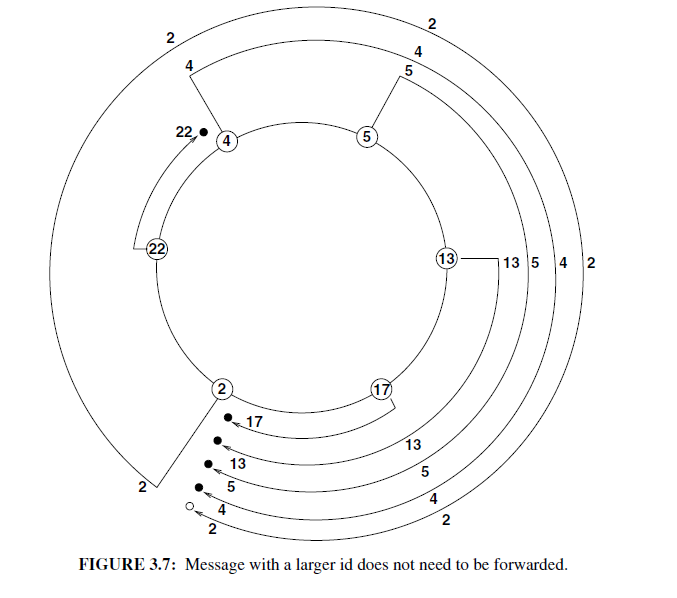
\includegraphics[scale=0.5]{images/asFar.png}
\end{center}

\begin{lstlisting} [caption={\textit{Protocollo AsFarAsItCan.}}]
Stati: S = {AVAIABLE, AWAKE, FOLLOWER, LEADER}
$S_{INIT}$ = {AVAIABLE}
$S_{FINAL}$ = {FOLLOWER, LEADER}
Restrictions = R, id, ring

AVAIABLE
    Spontaneously // evento spontaneo
    begin
        send("Election", id(x)) to right
        min := id(x) //il nostro valore
        become AWAKE
    end
    
    Receiving("Election", value) // evento istantaneo
    begin
        if value < id(x) then
            min := value
        else
        	min := id(x)
        send("Election", min) to other
        become AWAKE
    end

Procedure NOTIFY
    begin
        send("Notify") to N(x) \ sender
        become LEADER
    end

AWAKE
    Receiving("Election", value)
    begin
        if value < min then
            send("Election", value) to other //alla direzione opposta da dove e' arrivato
            min := value
        else
            if value = id(x)
                NOTIFY
            endif
        endif
    end
    Receiving("Notify")
    begin
        become FOLLOWER
        send("Notify") to other
    end
\end{lstlisting}

\textbf{Se mandassi il messaggio in entrambe le direzioni?}\\
Un altra idea potrebbe essere di mandare su tutte e due le direzioni e aspettare che uno solo dei due messaggi rivenga notificato all'entità che l'aveva mandato.\\
Purtroppo il lowerbound risulta come il precedente, poiché per il nodo con il minimo potrei avere $2n - 1$, quindi come numero messaggi siamo comunque nell'ordine di $n^2$, come tempo invece siamo scesi a $n/2 + n$.

\textbf{Costo del numero di Messaggi:} Il caso peggiore è uguale all'All The Way asintoticamente, ma si risparmiano alcuni messaggi.
$$\sum_{i=1}^{n} i = \frac{n(n+1)}{2} =  \in O(n^2)$$

\textbf{Costo del Tempo:} $n/2 + n$\\


\subsection{Controlled Distance}
Sviluppiamo ora un algoritmo che permetterà di risolvere il problema della Leader Election con un costo di $O(n \log n)$ per il numero di messaggi. Un'entità manda un messaggio di FORTH contenente la sua candidatura nella due direzioni, ma entro una distanza limitata. L'entità che invia la candidatura cercherà quindi di diventare leader di una porzione di rete, se quel messaggio arriva alla distanza prefissata, l'entità in quella posizione manda un messaggio di BACK. Se l'entità riceve 2 messaggi di BACK significa che è il minimo in quella porzione. Se così fosse allora incrementa la distanza iniziando un nuovo \textbf{stage}, l'obiettivo è quello di diventare leader di tutto il ring.\\
Un'entità diventa DEFEATED se riceve un messaggio avente id più piccolo del suo. Anche se è sconfitta partecipa comunque al protocollo effettuando il forwarding dei messaggi delle altre entità ancora in gioco.\\
Se un'entita in stato di CANDIDATE riceve un messaggio con un id più piccolo del suo diventa automaticamente Defeated indipendentemente dallo stage in cui è. Se un messaggio torna indietro dall'entità che lo ha inviato ma quell'entità nel mentre è diventata Defeated allora il messaggio viene semplicemente terminato.\\ Nel caso in cui uno o entrambi i messaggi di BACK non ritornano indietro l'entità non incrementa il proprio stage, quindi prima o poi riceverà un messaggio avente id più piccolo del suo diventando DEFEATED.\\
\textbf{Correttezza:}\\
%Siamo sicuri che questo algoritmo terminerà perché $dis$ è crescente quindi prima o poi il detentore del minimo si sveglierà ed il suo messaggio "FORTH" gli tornerà indietro e diventerà LEADER. Un'entità che non ha l'id minimo prima o poi incontrerà un'entità con un id minore del suo e quindi anche se fosse candidata non riceverà due messaggi di BACK e quindi non potrà iniziare un nuovo stage. Rimanendo bloccata prima o poi riceverà un messaggio avente id minore del suo, e diventerà DEFEATED.
La correttezza dell'algoritmo segue dalla funzione $f: stage \longrightarrow distanza $. Il messaggio contenente Id minimo attraverserà sempre un'entità, indipendentemente dal suo stato (ricordiamo che un'entità in stato di $candidate$ se riceve un messaggio con id più piccolo diventa automaticamente $defeated$). Quando la distanza che l'entità avente id minimo può raggiungere diventa $n$ il messaggio con id minimo viaggia su tutto il ring e quell'entità riuscirà a diventare LEADER e tutte le altre saranno Defeated.

%Libro: Un'entità x genera un messaggio con il proprio id e questo messaggio attraversa il Ring in entrambe le direzioni fin quando o viene terminato o quando raggiunge una cerca distanza $f$; se il messaggio non viene terminato si ritorna un messaggio di "return" all'entità che lo ha spedito. Quando arriva, quell'entità sa di essere quella con l'id minore in quella parte di ring delimitata dalla distanza $f$.\\
%%Idee:\\
%%\vspace{-10mm}
%\begin{itemize}
%\item Distanza limitata: L'entità imposterà un limite sulla distanza di invio del messaggio.
%\item Messaggi di ritorno: Se durante l'attraversamento dell'intervallo limitato il messaggio non viene terminato da nessuna entità, in ambe le parti, avente id minore allora si invierà il return al nodo originario per "concedere" l'autorizzazione ad allungare la distanza possibile.
%\item Spedisco e verifico su entrambi i versi
%\end{itemize}
\begin{center}
  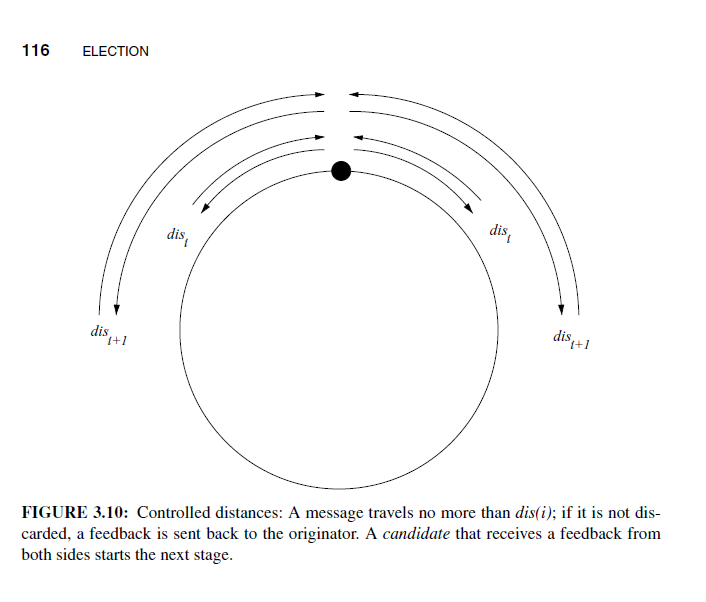
\includegraphics[scale=0.5]{images/controlled.png}
\end{center}
Se si inizia un nuovo Stage, il numero delle entità prese in considerazione sarà sicuramente maggiore di quelle dello stage precedente, quindi la funzione è monotona crescente. ($dis(i) > dis(i-1)$).

Riassumendo:
\begin{itemize}
\item in ogni stato elettorale ci sono alcuni candidati
\item ogni candidato manda un messaggio in entrambe le direzioni con il proprio id
\item un messaggio viaggia sul ring fin quando non incontra un id più piccolo o raggiunge la distanza prefissata
\item se un messaggio non incontra id più piccoli torna all'entità originante
\item infine un candidato che riceve entrambi i suoi messaggi in BACKWARD inizia un nuovo stage
\item se un candidato riceve un messaggio (di FORTH) nella direzione opposta a quella a cui l'aveva mandato allora diventa LEADER e lo notifica
\item se un candidato riceve un messaggio con ID più piccolo, diventa DEFEATED indipendentemente dallo stadio in cui si trova
\item un entità sconfitta inoltra i messaggi delle altre entità quando necessario, se il messaggio è la notifica lo inoltra e poi termina.
\item Se un'entità è in stato di ASLEEP e riceve un messaggio di FORTH da un'altra entità ma il suo $id$ è minore di quello all'interno del messaggio di Forth, allora si cambia stato in CANDIDATE, e si inizia il protocollo.
\item Se un'entità è in stato di ASLEEP e riceve un messaggio di FORTH da un'altra entità ma il suo $id$ è MAGGIORE di quello all'interno del messaggio di Forth, allora si cambia stato in PASSIVE, e l'unica cosa che si fa è che si inoltrano i messaggi che arrivano.

\end{itemize}
Tipi di messaggio:\\
\vspace{-10mm}
\begin{itemize}
\item Messaggio di candidatura, FORTH
\item Messaggio di back, BACK
\item Messaggio di notifica, NOTIFY, che viene spedito in una singola direzione.
\end{itemize}
Stati possibili delle entità nel protocollo:
\begin{itemize}
    \item ASLEEP (in p\_{init} tutte le entità sono in questo stato)
    \item CANDIDATE
    \item DEFEATED
    \item FOLLOWER
    \item LEADER
\end{itemize}
Un'entità inizia la propria esecuzione nello stato di ASLEEP. Cambia stato in CANDIDATE mediante impulso spontaneo e diventa DEFEATED se riceve un ID più piccolo del suo.\\
Il costo dell'algoritmo dipende totalmente dalla scelta della funzione $f$ utilizzata per determinare la massima distanza in cui viene inviato un messaggio "Forth" in un determinato Stage.
\subsection{Costo dei messaggi}
\textbf{con $i>1$}\\
%Per avere una stima dei messaggi invece useremo il parametro $n_i$ che indica le entità sopravvissute allo stadio $i-1$, cioè le entità che erano candidate e sono arrivate allo stadio i-esimo. Vediamo perchè questo valore è: $n_i \leq \big\lfloor \frac{n}{dis(i-1)+1} \big\rfloor$\\
\textbf{Calcoliamo il massimo numero di entità candidate ad arrivare allo stage $i-esimo$ $n_i$:}
Queste entità sono tutte quelle che hanno superato lo stage $i-1$. Per essere sopravvissute, l'id dell'entità $x$ deve essere minore di tutti i suoi vicini a distanza $dis(i)$ in entrambe le parti del ring. Quindi in ogni gruppo di $dis(i) + 1$ entità consecutive, al più una sopravvivrà lo stage $i-1$ ed inizierà lo $stage(i)$. Fondamentale che tra due entità in stato di Candidate ci sono esattamente $dis(i)$ entità comuni. [VEDERE DISEGNO SUL QUADERNO] \\
Ora, quanti insiemi posso avere in un ring? n proprio come il numero delle entità quindi disequazione:

$$(dis(i-1)+1) * n_i \leq n$$
$$n_i \leq \frac{n}{dis(i-1) + 1}$$

\textbf{Calcolo dei messaggi allo stage(i):}\\
Un'entità che inizia lo $stage(i)$ invierà il messaggio di "FORTH" in entrambe le direzioni, ogni messaggio viaggerà al più $dis(i)$ di distanza, per un totale di $2n_i(dis(i))$ numero di messaggi. Esaminiamo ora il messaggi di "BACK": Ogni entità che sopravviverà a questo stage riceverà tale messaggio in entrambe le direzioni, le entità che sopravvivranno allo stage(i) sono $n_{i+1}$, quindi aggiungeranno al totale dei messaggi inviati un $2n_{i+1}dis(i)$ messaggi. Ogni entità che inizia ma \textbf{non} sopravvive allo $stage(i)$ riceverà o un NO o un singolo messaggio di "BACK", causando un costo di \textbf{al più} $dis(i)$ messaggi. Il numero di queste entità è $n_i - n_{i+1}$ quindi il numero di messaggi in questo caso sarà  $(n_i - n_{i+1})dis(i)$. In totale le trasmissioni di messaggi di "BACK" saranno al più $2n_{i+1}dis(i) + (n_i - n_{i+1})dis(i)$.\\
\textbf{Riassumendo}, il numero totale di messaggi inviati allo $stage(i) > 1$ è:
\begin{center}
    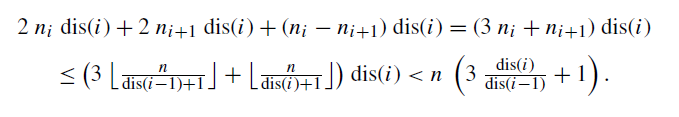
\includegraphics[scale=0.6]{aa/bb.png}
\end{center}
Posso mettere il $<$ perchè tolgo il $+1$ sotto, questo mi permette di semplificare ed infatti viene sempre solamente $+1$.


\subsection{Numero di messaggi inviati al primo Stage (quindi i = 1)}
Il primo stage è differente, poichè ogni entità può essere CANDIDATE; le $n_2$ entità che sono sopravvissute a questo stage avranno causato che i messaggi contenenti il loro id avranno viaggiato a distanza $dis(1)$ sia per i messaggi di FORTH che per i messaggi di BACK, causando $4n_2dis(1)$ messaggi. Le $n-n_2$ entità che non sopravvivranno a  questo stage causeranno un costo di al più 3 messaggi ognuno, poichè avremo 2 messaggi di FORTH ed uno solo di BACK nel peggiore dei casi, quindi avremo $3(n - n_2)dis(1)$ messaggi. Quindi il primo stage costa:
\begin{center}
    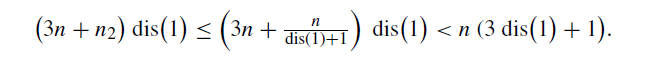
\includegraphics[scale=0.6]{aa/cc.png}
\end{center}
Perchè in questo caso $n_2 = n_i$ e quindi il valore può essere sostituito tenendo conto del $dis(1)$.\\
\textbf{Calcolo finale:}
Per trovare il numero di messaggi è necessario essere a conoscenza del numero totale $k$ di stages. Sappiamo che il leader sarà eletto appena il messaggio con id più piccolo effettua un giro intero del ring, quindi quando $dis(i) \geq n$. In altre parole, $k$ è il più piccolo intero tale che $dis(k) \geq n$. Tale intero è chiamato pseudo-inverso di n ed è denotato da $dis^{-1}(n)$.
Quindi il numero totale di messaggi utilizzati dal protocollo \textbf{Control\_Distance} è al più:
\begin{center}
    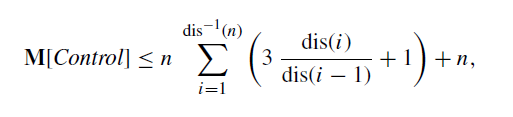
\includegraphics[scale=0.6]{aa/dd.png}
\end{center}
Dove:
\begin{itemize}
    \item $dis(0)$ = 1.
    \item Il $+ n$ finale è il messaggio per la notifica.
\end{itemize}

Per finalizzare il costo bisogna scegliere la funzione $dis$:\\

\textbf{Funzione Esponenziale: $dis(i) = 2^{i-1}$} e $dis^{-1}(n) =log(n) + 1$
$$\sum_{i=1}^{log(n) + 1 }n(3\frac{2^{i-1}}{2^{i-2}} + 1) = \sum_{i=1}^{log(n) + 1 }n(3 * 2^{i-1-i+2}+1) =  7nlogn$$
Con la scelta opportuna di $dis$ quindi siamo riusciti a migliorare il worst case portandolo a $O(nlogn)$.\\
\textbf{Parole del prof:} Se ci limitiamo a funzioni che fanno un risultato costante al rapporto $\frac{dis(i)}{dis(i-1)}$, il buond migliore è dato per $f(i) = 3^i$ e viene $6.309 n log n + n$.
\subsection{Tempo}
Il tempo richiesto dallo $stage(i)$ è il tempo necessario al messaggio contenente l'id più piccolo per arrivare alla distanza prefissata e tornare indietro dal suo mittente. Quindi esattamente $2dis(i)$ unità di tempo necessarie. Un addizionale $n$ va aggiungo sia per la notifica finale, sia per il wake-up iniziale dell'entità avente il minimo id. Questo quindi comporta che il tempo totale del protocollo è:
\begin{center}
    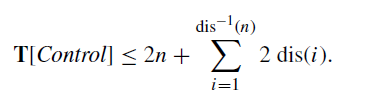
\includegraphics[scale=0.6]{aa/ee.png}
\end{center}
Anche qui dipende dalla scelta della funzione $dis$.\\
\textbf{Funzione Esponenziale: $f(i) = 2^{i-1}$}\\
Il tempo con questa funzione sarebbe O(n).

\begin{comment}


\textbf{Poniamo} dis(1) = Infinito
$$T[Control\_dis,Ring,R,id] \leq n + \frac{n}{2} + \frac{n}{2}$$
dove:
\begin{itemize}
    \item n è per il primo giro (trovare il minimo)
    \item $\frac{n}{2}$ per trovare il più piccolo nel caso non fosse sveglio
    \item $\frac{n}{2}$ per la notifica
\end{itemize}
\textbf{Poniamo $dis(1) = n/2$.}\\
 $T[$\texttt{Control}$] = \frac{n}{2} + 2n + n$
 \begin{itemize}
     \item $\frac{n}{2}$ per il wake-up
     \item $2n$ perché i 2 messaggi FORTH del minimo devono fare tutto il giro
     \item $n$ per la notifica
 \end{itemize}
 
\textbf{Poniamo $dis(1)=n$} allora $T[$\texttt{Control}$] = \frac{n}{2} + n + n$.\\In questo caso si ha il problema che all'inizio del protocollo non si conosce il numero delle entità, si può usare un trucchetto che è quello di porre $dis(1)$ a infinito.
\end{comment}

\begin{footnotesize}
\textbf{Nota: }
a scopo informativo, esiste un protocollo chiamato \emph{Stages} con un bound di $2n log n$, in pratica questo protocollo funziona che ad ogni passo dimezza sempre il numero di candidati
\end{footnotesize}

\section{Election su Griglia}
Trattiamo adesso il problema dell'Election su Griglia.
Una griglia di dimensioni $n = a \times b$ ha $a \cdot b$ nodi in cui il generico nodo ha 4 vicini, tranne quelli ai bordi che ne hanno 3 e quelli negli angoli che ne hanno 2.\\
In una griglia rettangolare si avranno sempre:
\begin{itemize}
    \item 4 angoli: entità con grado 2
    \item $2(a+b-4)$ entità di bordo con grado 3. Dove a sono le colonne mentre b sono le righe. il 4 non sono i 4 angoli della griglia, ma sono i 2 angoli della prima colonna e i 2 angoli della prima riga, nella figura sottostante $x_{1,1}$ viene presa in considerazione quindi due volte.
    \item (a-2)(b-2) entità interne aventi grado 4
\end{itemize}
\begin{center}
      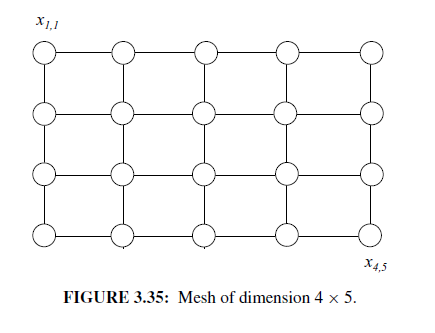
\includegraphics[scale=0.7]{images/griglia.png}
\end{center}

La simmetria di una griglia può essere utilizzata a nostro vantaggio per il problema della Leader Election. Poichè non importa quale entità diventi leader, possiamo eleggere uno dei quattro angoli. In questo caso, il problema dello scegliere il leader su n entità si riduce a trovare il leader tra 4 entità. L'idea quindi è quella di restringerci alla candidatura solo per gli angoli e far passare messaggi solo sul bordo così in pratica è come avere un ring.
Ci sono però alcune accortezze da considerare:
\begin{enumerate}
    \item Un initiator non è detto che stia sul bordo.
    \item Se così fosse la prima fase sarà il wake-up così da svegliare tutti i nodi compresi gli angoli, che poi faranno le loro candidature tramite l'All the Way o l'As\_far o protocollo Stage.
\end{enumerate}
\section{Costruzione del protocollo per Leader Election su Griglia}
Date queste accortezze il protocollo consisterà in:
\begin{itemize}
    \item wake-up che parte dagli iniziatori.
    \item fase di election sul "ring" esterno iniziata dai nodi angolo.
    \item Broadcast della notifica iniziata dal Leader che ha vinto.
\end{itemize}
Nella fase di election gli angoli spediscono in entrambe le direzioni, se chi riceve è un'entità di grado 2 o 3 allora continua il protocollo, se invece ho grado 4 (sono interno) o ignoro il messaggio o gli rispondo che sono un nodo interno e che quindi non mi verranno più inviati messaggi.\\
\subsection{Sviluppo del protocollo}
\begin{enumerate}
    \item Wake-up: Ogni $k^*$ iniziatore invierà un messaggio di Wake-up a tutti i suoi vicini, un nodo generico invece che riceverà un messaggio di sveglia da uno dei suoi vicini lo ripagherà a tutti tranne la porta dove lo ha ricevuto, dato che siamo su una griglia i messaggi inviati da ogni nodo non potranno essere più di 3. Per un totale di $3n +k^*$ messaggi inviati.
    \item Elezione su RING e messaggi errati: Bisogna scegliere sia quale protocollo utilizzare, sia come gestire i messaggi errati all'interno. Per la gestione, si fa in modo che un'entità invii il messaggio su entrambi le porte, quindi una sicuramente sarà quella del ring, mentre l'altra si gestisce l'errore. Questo farà in modo che l'entità interna che risponde, utilizzi 1 singolo messaggio, ma così facendo si fa in modo che l'entità nel ring non invii più messaggi errati a quella interna.
    \item Broadcast di Notifica: Si può utilizzare il Flooding, che se iniziato da uno dei 4 nodi costa $3n$.
\end{enumerate}
Da notare che l'azione più dispendiosa è il wake up iniziale.

\subsection{Calcolo del corso dei Messaggi}
Il numero di Collegamenti all'interno di una griglia è:
$$m=a(b-1)+b(a-1)$$
$M[grid\_leader,R,id,grid] \leq $ wake\_up + elezione + messaggi sbagliati verso l'interno + notifica in broadcast\\
Mettiamoci nel caso peggiore, ovvero che a svegliarsi sia un nodo interno e che vengano anche spediti messaggi ai nodi interni dal ring esterno, così da appunto mandare messaggi inutili.
\begin{itemize}
    \item Costo del Wake Up: Abbiamo $2(m)$ ma in questo caso $m = 4+3(a+b-4)+2(a-2)(b-2)$.
    \begin{itemize}
        \item $4$ indica gli angoli
        \item 3(a+b-4) indica i nodi di bordo
        \item 2(a-2)(b-2) indica i nodi interni
    \end{itemize}
    \item costo dell'elezione: Utilizziamo il protocollo stage, dato che l'elezione è come se avvenisse su un Ring. La proprietà dello stage è che il numero di candidati vengono dimezzati quindi avremmo $2n'$ come costo. Siano $n'$ i nodi posti solamente sul ring; essi sono un numero pari a $2(a+b-2)$. Considerando anche in questo caso gli errori che vengono commessi, un costo addizionale di $2(a+b-4)$ messaggi saranno inviati dal bordo verso i nodi interni, che dovranno rispondere un "Non mandarmi più messaggi perchè hai sbagliato" e quindi la risposta costa altri $2(a+b-4)$ messaggi. In conclusione il numero di messaggi che verranno inviati in questa fase sono:
    $$4(a+b-2)+2(a+b-4) = 6(a+b)-16$$
    \item Broadcast della notifica: Dato che sappiamo che l'UI è esattamente un angolo, esso invierà sempre 2 messaggi. un nodo generico manda la notifica in broadcast sempre su due link poichè i nodi interni aspettano esattamente due notifiche, ogni nodo quindi manda esattamente due messaggi. Così facendo il costo del broadcast è esattamente $2n$.\\\\La notifica costa: $2m - n +1 = 2 (2ab -b-a) -ab +1 = 3ab-2a-2b+1 \approx 3n$\\
Per la notifica si può fare che i nodi sul bordo inviano solo 2 messaggi, quelli interni aspettano l'arrivo di 2 messaggi e poi ne inviano altri 2, sugli archi da cui non gli sono arrivati. Quindi possiamo scendere a $2n$ messaggi per la notifica.
\end{itemize}
In conclusione, la fase più dispendiosa è il Wake Up iniziale che costa $4n$\\\\
Se a svegliarsi non sono i nodi sul bordo, essi andranno svegliati tramite un wake-up.\\
$m = a(b-1) + b(a-1)$, quindi per il wake-up si spenderebbero all'incirca $2n$ messaggi.

Per far viaggiare il protocollo di Leader Election solo sul bordo si potrebbe fare che i nodi esterni, quando ricevono un messaggio di candidatura, inviano 2 messaggi nei link rimastigli, uno rimarrà quindi nel bordo e proseguirà nel protocollo, l'altro direzionato all'interno della griglia verrà quindi ricevuto da un entità che sa di essere un nodo interno, ignorerà quindi il messaggio.

Se un entità riceve un messaggio di BACK sa che esso proviene da un entità di bordo e quindi potrà conoscere la sua effettiva situazione degli archi.

Se applichiamo \emph{Stages} avremo $\mathcal{O}(2n' \log n')$ con $n' = 2a + 2b - 4$ e con 2 stadi elettorali abbiamo eletto il leader.

\section{Election su Grafi Completi}
Affrontiamo adesso il problema della Leader Election con una topologia a grafo completo. Se usassimo un algoritmo standard saremmo nell'ordine di $n^2$. Risolvere la leader election ha come conseguenza diretta quella di risolvere il wake-up, il lower-bound per questo nei grafi completi avevamo visto essere $\Omega(\frac{1}{2}n \log n)$ tramite la tecnica dell'avversario.\\
\textbf{Insieme delle restrizioni:} Insieme standard per l'elezione. $(R+ID)$\\
Per costruire un protocollo più efficiente per l'ELECTION in un grafo Completo utilizzeremo una tecnica chiamata \textbf{Territory Acquisition.}\\
L'insieme degli stati in questa tecnica è il seguente:\\
\textbf{Stati:} \{LEADER, FOLLOWER, ASLEEP, CANDIDATE, PASSIVE, CAPTURED\}\\
\textbf{Descrizione a parole:}
In questa tecnica abbiamo un certo numero di candidati dove ognuno di essi prova a "catturare" i suoi vicini \textbf{uno alla volta} tramite l'invio di messaggi "CAPTURE" contenenti l'id del mittente ed il numero di nodi catturati fino ad ora (lo \textit{Stage)}. Se il tentativo va a buon fine, l'entità che ha ricevuto il messaggio diventa "Captured" e il candidato entra in un nuovo Stage continuando la sua esecuzione. Altrimenti il candidato diventa "Passivo". Trattandosi di un protocollo sequenziale, ovvero che una singola entità alla volta può essere conquistata da un'altra in stato di CANDIDATE, e trovandoci su grafo completo, appena un'entità possiede uno stage di valore $\frac{n}{2} +1 $ allora cambia stato in LEADER ed invia un messaggio di "notifica" a tutti i suoi vicini (ovvero a tutte le entità del sistema dato che siamo su grafo completo). Fondamentale il fatto che se due entità hanno lo stesso stage, allora vince chi ha l'id più PICCOLO.\\ 
Riassumendo: Un'entità in un qualsiasi momento può essere "Candidate", "Captured" o "Passiva". Un'entità Captured ha in memoria \textbf{l'id, lo stage} ed il collegamento al suo "possessore", ovvero l'entità che l'ha catturata. Le entità che sono CANDIDATE lo diventano tramite impulso spontaneo in stato di ASLEEP.
Di seguito le \textbf{regole formali:}
\begin{enumerate}
\item Un entità candidata x manda un messaggio di CAPTURE ad un suo vicino y (che non fa già parte del territorio di x)
\item Se y è passivo o Asleep l'attacco ha successo. x incrementa il suo stage ed y diventa Captured.
\item Se y è "CANDIDATE", il risultato dell'attacco dipende dallo stage e dall'id delle due entità:
\begin{itemize}
    \item Se $stage(x) > stage(y)$, l'attacco ha successo. x incrementa il suo stage ed y diventa Captured.
    \item Se $stage(x) = stage(y)$, l'attacco ha successo se $id(x) < id(y)$ altrimenti $x$ diventa passivo.
    \item Se $stage(x) < stage(y)$, x diventa passivo.
\end{itemize}
\item Se y è "CAPTURED" allora x deve sconfiggere il padrone di y, che chiameremo z, prima di poter catturare y. Se così fosse, y manda a z un messaggio di WARNING con stage(x) e l'id(x) e:
\begin{itemize}
\item Se z è candidato in uno stage più alto o nello stesso stage di x ma $id(z) < id(x)$ allora l'attacco a y da parte di x non ha successo. z quindi lo notifica a y che lo notifica a x.
\item In tutti gli altri casi (ovvero se z è già stato a sua volta catturato, se z è passivo, se z è un "Candidate" in uno stage più piccolo o ha lo stesso stage di x ma con id più grande di x) l'attacco ha successo; z lo notifica a y che lo notifica a x e se z era candidato diventa passivo (dato che z poteva già essere "Passivo").
\end{itemize}
\item Se l'attacco ha successo, y è catturata da x, x incrementa il suo $stage(x)$ e continua l'esecuzione della sua conquista.
%\item Quando una delle entità diventa il leader, lo notifica tramite broadcast a tutte le altre.
\end{enumerate}
Al protocollo va aggiunta poi la notifica finale.
\\
\subsection{Costo dei Messaggi}
Da notare che ogni tentativo effettuato da un Candidato ad un vicino anch'esso "Candidato" o "Passivo" costa esattamente due messaggi:
\begin{itemize}
    \item Uno per "Capture".
    \item Uno per la Notifica.
\end{itemize}
Se invece il suo vicino è già stato Catturato, due messaggi addizionali verranno inviati:
\begin{itemize}
    \item Uno dall'entità già catturata al suo padrone.
    \item Il messaggio di ritorno dal Padrone all'entità.
\end{itemize}
Questo metodo risolve quindi il problema dell'elezione sui grafi completi.

\subsection{Descrizione a parole del protocollo}

\begin{itemize}
    \item \textbf{AVAIABLE:} Se ricevi impulso spontaneo allora fissa lo stage = 1, il valore = id(x) e crea l'insieme "others" che contiene tutto il tuo vicinato. Scegli un nodo dentro questo insieme ed invia il messaggio di Capture a quest'ultimo allegando il suo stage ed il tuo id. Successivamente diventa CANDIDATE.\\
    Se invece non ti svegli tramite impulso spontaneo ma ricevi un messaggio di Capture da Avaiable allora invia immediatamente il messaggio di accettazione salvando l'entità che è tua "padrona", il tuo stage che è = 1 e lo stage del tuo padrone +1 (puoi vedere questo valore perchè te lo ha inviato all'interno del messaggio). Successivamente cambia stato in CAPTURED.
    \item \textbf{CANDIDATE:} Se ricevi un messaggio di tipo "Capture" allora fai tutti i controlli sopra. Da notare che se chi attacca vince questa entità diventa CAPTURED.\\
    Se invece ricevi un messaggio di "ACCEPT" allora incrementa il suo stage e controlla subito se questo valore è $\geq \frac{n}{2} +1$. Se cosi fosse invia la notifica a tutti i tuoi vicini (che sono tutte le entità dato che siamo su un grafo completo) e diventa Leader. 
    Altrimenti il tuo stage non è grande a sufficienza per vincere, prova quindi ad inviare un altro messaggio di Capture ad un altro dei tuoi vicini.
    \item \textbf{Candidate:} Se ricevi il messaggio di "reject" cambia stato in PASSIVE. \\ Se ricevi il messaggio di "Terminate" cambia stato in FOLLOWER.
    \\ Se ricevi uno "Warning" significa che un'entità sotto il tuo controllo è stata attaccata da un altra in stato di CANDIDATE, effettua i controlli sopra ed invia "NO" o "YES" in base a questi.
    \item \textbf{Passive:} Se ricevi un messaggio di CAPTURE hai comunque in memoria lo stage dell'ultima entità che ti ha conquistato, quindi controlla comunque se lo stage e l'id dell'entità che prova a conquistarti ora sono validi (fai i controlli precedenti). Se i controlli vanno a buon fine diventa nuovamente CAPTURED salvando lo stage del tuo possessore e quale è il tuo possessore.
\end{itemize}

\subsection{Calcolo del costo}
\'E necessario tenere traccia di quanti candidati possono essere presenti allo $stage(i)$. Rappresentiamo questo valore con $n_i$. Per calcolare questo valore però è necessario assicurare che un nodo venga catturato da al più 1 candidato nello stesso stage.\\
\textbf{Vediamo un esempio del problema del protocollo appena enunciato:}\\
Supponiamo quattro entità x, y, z, w; x e y sono nello stesso stage e z è catturata da w.\\
Se sia x che y mandano un messaggio di candidatura a z, questa allora manderà un WARNING a w e verrà poi notificata la risposta, supponiamo poi che prima che arrivi il messaggio di notifica, z processa anche y e manda quindi un altro WARNING a w, a questo punto abbiamo 2 notifiche da parte di w, queste possono essere entrambe positive. Ci ritroveremmo quindi che sia x che y hanno conquistato z, ma secondo z essa è legato solo all'ultima processata, quindi y.\\
\subsubsection{Risoluzione del problema:}
Possiamo ovviare a questo problema mettendo un buffer nelle entità.
Facciamo in modo che i messaggi di Warning siano inviati uno alla volta e solamente al vero padre dell'entità che sta venendo conquistata
Facciamo in modo un'entità aspetti dopo un WARNING quale sia la risposta ricevuta, così nello stesso caso di sopra la nuova domanda (di y) sarebbe stata mandata al vero candidato, cioè x.\\
Apportiamo le seguenti modifiche:
%S\vspace{-5mm}
\begin{enumerate}
\item Se un nodo catturato y riceve un messaggio di CAPTURE da un candidato x che è in uno stadio più piccolo di quello conosciuto da y, allora y notifica immediatamente a x che l'attacco non ha avuto successo (x diventa passivo). Di conseguenza, un nodo y catturato invierà solo WARNING per un attacco che ha stage più alto del suo. 
\item Se un nodo y manda un WARNING al suo padrone z riguardante un attacco di x, allora y aspetta la risposta da z prima di mandare eventuali altri WARNING.
\end{enumerate}
La conseguenza di questo secondo punto è che se un attacco da x ha successo (e quindi il suo stage viene incrementato) y invierà al nuovo padrone x qualsiasi WARNING successivo generato dall'elaborazione dei messaggi di cattura accodati. Dopo questa modifica, è garantito che il territorio di due candidati nello stesso stage non abbia nodi in comune.\\
\colorbox{yellow}{\textbf{Quanti candidati possono essere presenti allo stage i?}}\\
Ogni candidato ha un territorio di grandezza i e questi territori sono disgiunti, quindi non possono esserci più di $$n_i \leq \frac{n}{i}$$ candidati (Le entità vengono conquistate una alla volta, il protocollo è sequenziale). \\
\colorbox{yellow}{\textbf{Quanti messaggi inviano $n_i$ candidati allo $stage(i)$?}}\\
Ognuno darà origine ad un attacco che costerà al massimo 4 messaggi; quindi, nello stage i, ci saranno al più $$\frac{4n}{i}$$ messaggi. \\
\colorbox{yellow}{\textbf{Determiniamo ora il numero di Stage necessari per la terminazione del protocollo.}} \\
Consideriamo il seguente fatto: Se un Candidato ha conquistato un territorio di grandezza $$\frac{n}{2} +1$$, nessun altro candidato può diventare Leader. Quindi, un candidato può diventare leader appena raggiunge quello stage (successivamente fa il broadcast della notifica di "vittoria" a tutti gli altri nodi).\\
In conclusione, il numero totale di messaggi, incluso $n-1$ messaggi per la notifica finale in broadcast è il seguente:

$$ n-1 + \sum_{i=1}^{\#stadi} 4 n_i \leq n-1 + 4 \sum_{i=1}^{n/2} n_i = 4 n H_{n/2} + n + 1$$
Dove:
\begin{itemize}
    \item (n-1) è il costo della notifica in broadcast su un grafo completo, ovvero l'entità LEADER invia un messaggio a tutti i suoi vicini che sono $n-1$.
    \item La sommatoria indica i messaggi inviati dalle entità candidate allo stage(i) che sono appunto al più 4 per ognuna di esse.
    
\end{itemize}

Che da un costo complessivo di:
$$M[CompleteElection, R, id, K_n] \leq 2.76 n log n - 1.76 n + 1$$
Il costo del libro è il seguente:\\
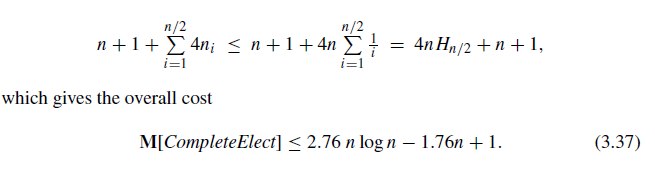
\includegraphics[]{images/fff.png}
Dal libro e dagli appunti presi a lezione, ne risulta che la serie è un'armonica crescente, che ha come risultato $nlogn$, credo che sia questo il $H_{n/2}$ sulla foto del libro.\\


\textbf{Siamo ottimi per i messaggi?}
SI! perchè il lower bound per QUALSIASI protocollo di Leader Election su grafo completo è $\Omega(n \log n)$ messaggi, dato che ha come sotto problema quello del Wake-Up, ovvero che tutte le entità, prima di eleggere il Leader devono necessariamente essere sveglie. Abbiamo visto tramite la tecnica dell'avversario che il Lower Bound per il Wake-up è $\frac{1}{2}n \log n$.


\textbf{Tempo:}\\ $$T[CompleteElection, R, id, K_n] \leq 4 \frac{n}{2} + 1 \leq 2 n$$
\begin{itemize}
    \item $ 4 \frac{n}{2} $ Perchè abbiamo 4 messaggi per stage nel caso peggiore.
    \item + 1 indica la notifica finale che, essendo in un grafo completo, costa una singola unità di tempo.
\end{itemize}

\textbf{Siamo ottimi per il tempo?} NO! perchè è possibile sviluppare un protocollo che ogni entità invia l'id a tutti i suoi vicini (che sono n-1 in un grafo completo) e poi tutti rispondono con un messaggio contenente il loro ID, così che ogni entità possa determinare se il suo è l'id minimo oppure no. In questo caso spediamo $O(1)$ tempo ma il costo dei messaggi va a $O(n^2)$.

\subsection{Miglioramento del protocollo Complete Election: tolgo la sequenzialità e riesco ad abbassare il tempo}
Il protocollo che abbiamo appena visto impone che ad ogni singolo stage un'entità possa conquistarne esattamente un'altra, quindi abbiamo in gioco il fattore della sequenzialità. Per effettuare una miglioria sul tempo è necessario ridurre il numero di stage. Per far questo però è necessario togliere la sequenzialità, ovvero fare in modo che in ogni stage un'entità deve cercare di conquistarne più di un'altra.\\
\textbf{Caso Estremo:} Abbiamo un singolo iniziatore che contatta tutti, il tempo in questo caso sarebbe $O(1)$ ma il numero dei messaggi salirebbe a $O(n^2)$. Ne risulta quindi che bisogna porre un limite sulle entità contattabili.\\
\textbf{Creazione dell'algoritmo migliore:} Vediamo adesso come creare un'algoritmo che ci consenta di avere $O(n \log n)$ messaggi e $O(\log n)$ tempo.\\
Facendo riferimento alle domande poste durante lo sviluppo del precedente protocollo:\\
\textbf{Quanto è il numero delle entità candidate contemporaneamente allora stage i-esimo?}: Esattamente $n_i$.
Se allora stage i-esimo si conquistano $2^i$ entità allora $n_i = \frac{n}{2^i}$. Così facendo il numero di messaggi inviati raddoppia ma il numero delle entità che li mandano dimezza, e quindi siamo restati sulla stessa complessità. Al più la metà delle entità che si sveglia passa allo stage successivo.
\begin{center}
    Costo dei Messaggi: $O(n \log n)$\\
    Costo del tempo: $O(\log(n))$
\end{center}

\chapter{Sistemi Sincroni}
Negli ambienti di calcolo distribuito che abbiamo considerato finora, non abbiamo fatto alcuna ipotesi sul tempo. Infatti, dal modello sappiamo solo che in assenza di guasto, un messaggio trasmesso da un'entità alla fine arriverà al suo vicino: l'\textbf{assioma dei Ritardi Finiti}. Non viene specificato altro, quindi non sappiamo ad esempio quanto tempo impiegherà una comunicazione. Nel nostro ambiente ogni entità è dotata di un orologio locale; ancora non viene fatta alcuna ipotesi sul funzionamento di questi orologi, sulla loro velocità e su come si relazionano tra loro o ai ritardi di comunicazione. Per questi motivi, gli ambienti di calcolo distribuito descritti dal modello di base sono comunemente indicati come \textbf{sistemi completamente asincroni}. Rappresentano un estremo nello spettro dei sistemi di scambio di messaggi rispetto al tempo.\\
Non appena aggiungiamo restrizioni temporali, facendo ipotesi sugli orologi locali e/o sui ritardi di comunicazione, descriviamo diversi sistemi all'interno di questo spettro.\\
All'estremo opposto ci sono i \textbf{sistemi completamente sincroni, ambienti di elaborazione distribuiti in cui vi sono forti ipotesi sia sugli orologi locali che sui ritardi di comunicazione}. Questi sistemi sono definiti dalle seguenti due restrizioni sul tempo: \textbf{clock sincronizzati e ritardi di trasmissione limitati}.

\textbf{Limitazione 6.1.1 Orologi sincronizzati} Tutti gli orologi locali vengono incrementati di un'unità contemporaneamente.\\
In altre parole, tutti gli orologi locali "ticchettano" simultaneamente. Si noti che questa ipotesi non significa che gli orologi abbiano lo stesso valore, ma solo che il loro valore viene incrementato allo stesso tempo. Si noti inoltre che l'intervallo di tempo tra incrementi consecutivi in generale non deve essere costante.\\
Per semplicità, nel seguito assumeremo che sia così e indicheremo con $\delta$ tale costante.\\

\textbf{Per convenzione},
\begin{enumerate}
    \item le entità trasmetteranno i messaggi (se necessario) ai loro vicini solo allo scoccare del ticchettio dell'orologio;
    \item ad ogni tick dell'orologio, un'entità invierà al massimo un messaggio allo stesso vicino.
\end{enumerate}

\textbf{Limitazione 6.1.2 Ritardi di comunicazione limitati} Esiste un limite superiore noto sui ritardi di comunicazione subiti da un messaggio in assenza di errori.\\
In altre parole, esiste una costante $\Delta$ tale che, in assenza di guasti, ogni messaggio inviato all'istante $T$ arriverà e sarà elaborato all'istante $T + \Delta$. In termini di tick dell'orologio, ciò significa che in assenza di errori, ogni messaggio inviato al tick dell'orologio locale $t$ arriverà e sarà elaborato dal tick dell'orologio $t + \lceil \frac{\Delta}{\delta} \rceil$ (ora del mittente).\\
Riassumendo, un sistema completamente sincrono è un ambiente informatico distribuito in cui valgono entrambe le restrizioni di cui sopra. Si noti che la conoscenza di $\Delta$ può essere sostituita dalla conoscenza di $\lceil \frac{\Delta}{\delta} \rceil$.

Il caso sincrono è quindi un caso particolare del caso asincrono, ma avrà due aspetti che possiamo sfruttare:
\begin{enumerate}
   \item L'allarme.
   \item Il silenzio: se un'entità non riceve nulla da un certo Edge (arco) per un certo periodo di tempo, può effettuare delle assunzioni. Questo non poteva accadere nel sistema asincrono poichè come restrizione avevamo che "prima o poi" un certo messaggio sarebbe sicuramente arrivato.  In un sistema sincrono invece, o il messaggio arriva ad un determinato tempo di clock o non arriverà mai.
\end{enumerate}

\section{Leader Election su Ring sincrono}
Prendiamo adesso in esempio il problema della Leader Election su un ring sincrono.\\
\textbf{Restrizioni:} Insieme Standard per L'elezione (IR) e Sync:
\begin{itemize}
    \item \textbf{Synchronized Clocks}: Tutti i clock sono incrementati di un'unità simultaneamente. Da notare che questo non significa che tutte le entità hanno lo stesso valore di clock, ma che il loro valore sarà incrementato allo stesso momento per tutte.
    \item \textbf{Unitary Communication Delays}: In assenza di fallimenti, un messaggio trasmesso arriverà e sarà elaborato al massimo in un tick di clock.
    %\item Bounded Communication Delays: Esiste un upperbound per i ritardi di comunicazione subiti da un messaggio in assenza di errori. Ovvero che posso fare delle assunzioni se il messaggio non arriva dopo un certo tempo.
    \item \textbf{Boundend Message}: Esiste una costante $c$ tale per cui ogni messaggio conterrà \textbf{al più $c$ bits}. Se non si riesce a spedire un messaggio in un singolo tick di clock allora si deve necessariamente suddividere in pacchetti.
\end{itemize}


\section{Protocollo Speed}
In questo protocollo viene eletto il LEADER solamente tra gli iniziatori. Tutte le entità che non ricevono un impulso spontaneo appena gli arriva un messaggio diventano RELAYER. Queste non origineranno nessun messaggio ma saranno comunque partecipi della leader election facendo aspettare i messaggi su di loro ed eliminandoli qualora ricevessero messaggi aventi id minori. Assumiamo poi che tutti gli id delle entità siano abbastanza piccoli da essere contenuti all'interno di un singolo pacchetto.
Stati del protocollo:
\begin{itemize}
    \item Stati: S = ASLEEP, CANDIDATE, FOLLOWER, LEADER, RELAYER
    \item        $S_{INIT}$ = ASLEEP
    \item        $S_{FINAL}$ = FOLLOWER, LEADER
\end{itemize}
Il protocollo che vedremo si basa sul protocollo \textbf{AsFar} con la caratteristica che i messaggi viaggiano a velocità differenti in maniera direttamente proporzionale rispetto alla grandezza del loro id. I messaggi con id minori quindi viaggiano a velocità maggiori, mentre i messaggi con id maggiore saranno "rallentati". Questo rallentamento è ottenibile sfruttando il sistema sincrono; possiamo fermare un messaggio su un'entità per quanto tempo vogliamo.\\
In questo nuovo protocollo un id verrà scartato se:
\begin{itemize}
    \item Incontra id più piccolo su un'entità.
    \item Viene "sorpassato" da un messaggio avente id più piccolo.
\end{itemize}
In un sistema sincrono però, ogni trasmissione di un messaggio prende al più una singola unità di tempo; quindi, tutti i messaggi verranno spediti alla stessa velocità.\\ \textbf{Come possiamo implementare le diverse velocità nei messaggi in base agli id?}\\
Assumiamo innanzitutto che la dimensione di un messaggio possa essere contenuta all'interno di un singolo messaggio, e che quindi non ci preoccupiamo della suddivisione in pacchetti. La risposta è la seguente:
\begin{itemize}
    \item Quando un'entità x riceve un messaggio con un valore $i$ minore di tutti gli altri visti fino ad ora (\textbf{perchè ci basiamo sull'AsFar quindi ogni entità manda l'id solamente se è minore del suo comunque)}, invece che effettuare immediatamente il forwarding del messaggio sul ring, $x$ trattiene questo messaggio per un certo periodo di tempo (ovvero per un certo numero di tick di clock). \textbf{Questo tempo d'attesa è tanto grande quanto più grande è l'id del messaggio}, ovvero in simboli, $f(i)$ (ovvero il tempo che aspetta, in tick di clock) è direttamente proporzionale ad $i$ (ovvero il valore dell'id).
    \item Se un messaggio con un id minore arriva a $x$ durante questo tempo d' attesa, $x$ rimuove $i$ dalle sue considerazioni ed effettua il processing del nuovo valore. Altrimenti, dopo aver trattenuto $i$ per $f(i)$ tick di clock, x effettua il forwarding del messaggio nel ring.
\end{itemize}

\textbf{FONDAMENTALE:}\\
\begin{center}
    Queste regole faranno in modo che un messaggio con valore $i$ viaggi all'interno del ring ad una velocità di $1+f(i)$.
\end{center}

\textbf{Esempi:} Se un messaggio arriva a tempo $0$ su un'entità, allora sarà rinviato dopo $1+f(i)$ tempo alla prossima entità, poi a tempo $2+2f(i)$, $3+3f(i)$ e si continua fin quando o viene scartato oppure completa il giro di tutto il ring. All'interno del codice questo è implementato tramite $c(x)+f(id).$

Più grande è il valore di un messaggio, ovvero $i$, più tempo aspetterà su una determinata entità. In conclusione, soltanto l'entità con id minimo passerà tutto il ring, tutte le altre invece, o incontreranno direttamente l'entità con l'id minimo, o verranno sorpassate da quest'ultimo; se così fosse l'entità che in quel momento riceve l'id più piccolo, uccide quello che aveva e si mette ad aspettare $1+f(i)$ tick di clock di quello che gli è appena arrivato. La correttezza del protocollo segue dal fatto che l'id più piccolo non verrà mai scartato da nessuna entità e ritornerà quindi all'entità che lo ha generato, quell'entità quindi diventerà LEADER.

\subsection{Calcolo del costo:}
\subsubsection{Numero di messaggi}
Le performance generali del protocollo descritto dipendono dalla funzione $f$ che si sceglie, bisogna quindi stimare il numeri di messaggi inviati in funzione di quest'ultima. Innanzitutto, il numero di messaggi generati dall'entità con id minimo saranno $2n$, poichè serve un $n$ per tutto il giro e serve un $n$ per il messaggio di notifica di "vittoria".\\
\textbf{Supponiamo adesso che siano tutti iniziatori e tutti in stato di "CANDIDATE"} e come funzione scegliamo \textbf{$f(id) = id$}. Calcoliamo quanti messaggi si avrebbero nel caso peggiore:\\
Quante entità riesce a superare il messaggio con id minimo? $n$\\
Quante entità riesce a superare il messaggio con il secondo id minimo? $n/2$\\
Quante entità riesce a superare il messaggio con il terzo id minimo? $n/3$\\
e così via, in totale quindi avremo: $$\sum_{i=1}^{n}\frac{n}{i} + n = O(n \log n)$$ questa serie è uguale al calcolo del costo di quella sulla territory acquisition. Scegliendo quindi la funzione $f(id) = id$ abbiamo migliorato il costo dell'AsFar da $n^2$ a $n \log n$. Intuitivamente più aumentiamo il ritardo e più il costo diminuisce, vediamo quindi un altra funzione.\\
$f(id) = 2^i$\\
Quante entità riesce a superare il messaggio con id minimo? $n$\\
Quante entità riesce a superare il messaggio con il secondo id minimo? $n/2$\\
Quante entità riesce a superare il messaggio con il terzo id minimo? $n/4$\\
In generale quindi si ha:
$$\sum_{i=1}^{n}\frac{n}{2^{i-1}}  +n = O(n)$$
Questo è possibile però se si assume che l'informazione dell'$id$ sia abbastanza piccola da essere contenuta in un singolo pacchetto. Ciò è corretto solamente se i valori in input sono limitati da $2^c$. Infatti all'interno dell'insieme delle restrizioni era presente anche \textbf{InputSize($2^c$).}\\
\textbf{Domanda di Francesco:}
\'E buono come costo? SI! perchè il lower bound per la leader election su Ring sotto le restrizioni di R ed ID era $\Omega(n \log n)$, mentre con la restrizione del $Sync$ siamo riusciti ad abbassare il lower bound.\\
\textbf{Tempo:}\\
Il costo del tempo in questo caso è esponenziale e sarà l'entità che ha id più piccolo a generare questo tempo: $$O(n 2^{id})$$
\textbf{Dim:} Consideriamo un'entità $x$ che diventerà Leader. Il suo messaggio ha viaggiato all'interno di tutto il ring alla velocità di $f(id)+1 = 2^{id}+1$ dove l'id è il valore dell'entità $x$. Questo messaggio torna a lei dopo $(n-1)(2^{id}+1)$ unità di tempo. A questo va aggiunto un $n$ per la notifica.\\
Il tempo è Super Esponenziale, ovvero che non è esponenziale in $n$ ma nel range dei valori di input $id$.\\

\begin{center}
    Lower Bound per la Leader Election su sistema \textbf{Asincrono} è:
    $$Messaggi: \Omega(n \log n) $$ $$Tempo: \Omega(n)$$
\end{center}

Si devono però confrontare i due casi peggiori. Quindi il caso peggiore gli ($O$). Nella leader election Asincrona si aveva che era $O(n \log n)$ qui invece siamo $O(n)$ quindi abbiamo migliorato. Per il tempo invece avevamo $O(n)$ ma qui siamo esponenziali e non va bene.

\textbf{Numero di bit:} $$B[speed] = O(n \log(id))$$
Dove:
\begin{itemize}
    \item Poichè ogni entità ($n$) contiene un $id$ che è rappresentato nel sistema come $\log(id)$. Le dimensioni dell'input sono $\log(id)$ come nel protocollo TwoBits. Dato che di $id$ ne ho $n$ allora avrò quel numero. 
\end{itemize}

\textbf{Confronto tra i Bound [Numero di Bit credo]:}
Il costo peggiore della Leader Election è $log(valore)$, ma su speed abbiamo $log(id)$. Il tempo nel caso dell'id Massimo (Ovvero quello ci metterà sempre di più) è $log^{id}$, che rispetto a quello $log(id)$ è pessimo.


Ricordiamoci che abbiamo assunto che tutte le entità si svegliano allo stesso momento, ma questa assunzione non è fondamentale, poichè possiamo effettuare un wake-up ed eleggere il leader solamente tra gli iniziatori spontanei del protocollo.

\subsection{Informazioni Aggiuntive sul protocollo}
 \textbf{Partecipano alla leader election solo gli iniziatori}, quindi i restanti non partecipano attivamente al protocollo.
 
 \begin{itemize}
     \item ASLEEP: Se ricevi impulso spontaneo allora invia il messaggio contenente il tuo id verso destra e diventa CANDIDATE.\\
     Se invece da questo stato ricevi un altro messaggio allora salvati il suo id e propaga questo messaggio dalla direzione opposta in cui l'hai ricevuto, poi diventa RELAYER.
     \item CANDIDATE: Se in questo stato ricevi un messaggio contenente un certo id, controlla se è più piccolo di quello conosciuto a te fino a quel momento. Se così fosse allora aggiorna il minimo e mettiti ad aspettare il tempo necessario per quel messaggio. Successivamente diventa RELAYER (quando il tempo è terminato rispedirai il messaggio nella direzione opposta in quello in cui l'hai ricevuto).\\
     Se invece l'id che ti è arrivato è proprio uguale al tuo allora diventa LEADER e notificalo tramite 1 singolo giro di ring scegliendo una direzione.\\
     Se il tempo che hai atteso per un messaggio è terminato allora propagalo nella direzione opposta di quella in cui l'hai ricevuto.\\
     Se ricevi la notifica diventa FOLLOWER.
     \item RELAYER: Se ricevi un messaggio avente un certo id, controlla se è più piccolo di quelli visti fino ad adesso. Se così fosse allora aggiorna il minimo locale e mettiti ad aspettare $c(x)+f(id)$ tick di clock. Quando questi sono passati allora invia il messaggio nella direzione opposta di quella in cui l'hai ricevuto.\\
     Se ricevi la notifica diventa FOLLOWER.
     
 \end{itemize}
 
\section{Protocollo TwoBits}

\theorem{
In assenza di guasti, ogni sequenza finita di bit (che chiameremo messaggio $\alpha$) può essere comunicata trasmettendo 2 messaggi indipendentemente dalla grandezza di questi.
}
\textbf{Dim:} Supponiamo sistema sincrono e due entità, x ed y; x deve inviare un messaggio $\alpha$ in binario a y. Indichiamo con $I()$ il casting in base 10 (intera) del messaggio. Prima dell'invio, a questo viene aggiunto un 1 davanti poiché se questo iniziasse con 0 ci sarebbe il rischio di perdere dati. Sia $I(1\alpha)$ il cast ad intero del messaggio $1\alpha$ (che sarebbe la sequenza binaria di $\alpha$ e l'1 davanti) consideriamo il seguente protocollo:
\begin{enumerate}
    \item Entità $x$:
    \begin{enumerate}
        \item Manda un messaggio (1 bit) a y con "Start-Counting".
        \item Aspetta $I(1\alpha)$ tick di click e poi:
        \item Manda un messaggio (1 bit) ad y come "Stop-Counting".
    \end{enumerate}
    \item Entità $y$:
    \begin{enumerate}
        \item Alla ricezione del primo bit con "Start-Couting" come messaggio, salva il valore corrente $c_1$ del suo clock.
        \item Alla ricezione del secondo bit con "Stop-Counting" come messaggio, salva il valore corrente $c_2$ del suo clock e calcola $c_2 - c_1$ che restituisce $I(1\alpha)$. A questo punto lo trasforma in binario, butta via il primo uno e ottiene nuovamente $\alpha$.
    \end{enumerate}
\end{enumerate}
Concludiamo affermando che è possibile spedire qualsiasi messaggio di qualsiasi dimensione tramite la trasmissione di soli 2 bits.\\
\textbf{Calcolo del costo:}\\
Precisamente, il "costo della comunicazione" di un protocollo P completamente sincrono è una coppia formata da $<P,T>$ dove P denota il numero di pacchetti, e T denota il numero di unità di tempo. La complessità quindi del protocollo Speed è la seguente:$$Cost[Speed(i)] = <O(n \log i), O(n 2^{id})>$$ mentre del protocollo 2bits è $$C[TwoBits(\alpha)] = <2, O(2^{|\alpha|})>$$ $$|\alpha|=\log_2(I(1\alpha))$$
Il tempo di attesa è $I(1\alpha)$ e la dimensione dell'input è $log_2 I(1\alpha)$, però più cresce $1\alpha$ e più tempo sarà necessario per l'invio, perciò \textbf{il tempo è esponenziale rispetto la dimensione dell'input.}
\\
\textbf{Domande del professore:}\\
Posso fare meglio per il numero dei messaggi? No, siamo ottimi.\\
Perchè il tempo è $2^{|\alpha|}$? Intanto $|\alpha|$ è la dimensione dell'input. Il tempo d'attesa è esattamente $I(1\alpha)$, ma all'interno del sistema il tempo è $log(I(1\alpha))$ quindi per ottenerlo devo elevarlo al quadrato.\\
(Dalla ragistrazione:) Mentre nei sistemi Asincroni il tempo che siamo è una stima, nei sistemi Sincroni il tempo che diamo è esattamente il tempo che ci mette il protocollo a terminare correttamente.


\chapter{Gathering}
\emph{R. Kalsing, E. Markou, A. Pelc - Gathering Asynchronous Oblivious Mobile Robots In A Ring}

\textbf{Problema del Gathering:} Convogliare un insieme di robots posizionati tutti in un differente nodo all'interno di un grafo in un singolo nodo.\\
Nel nostro caso abbiamo studiato, all'interno dell'articolo, il problema del Gathering in una topologia \textbf{RING} non orientata. In questo caso le assunzioni che facciamo sono le seguenti:
\begin{itemize}
    \item Ogni robot all'inizio della computazione si trova su un nodo distinto.
    \item Ogni robot fa le proprie scelte localmente (\textbf{Autonomous}).
    \item I robot non hanno un identificatore univoco, quindi non hanno id che li distingue (\textbf{Anonymous}).
    \item Sono omogenei, tutti quanti eseguono lo stesso algoritmo deterministico.
    \item sono Oblivi, ovvero non hanno memoria (\textbf{Oblivious}).
    \item Sono silenti, ovvero non hanno nessun modo di comunicare esplicitamente tra di loro (tipo attraverso connessioni wireless) (\textbf{Silent}).
    \item Sono non-orientati, ovvero i robot non hanno modo di concludere se un nodo si trova a nord o a sud della loro posizione e quindi non concordano tra di loro su un determinato sistema di coordinate.
    \item Sono Asincroni
    \item Ogni robot si sveglia in un tempo finito e infinite volte.
    \item Multiplicity detection capability: Durante la fase di Look, che vedremo successivamente, i robot possono vedere un nodo che contiene più di un robot (chiamata, appunto, molteplicità). Esistono quattro tipi di molteplicità:
    \begin{itemize}
    \item \textbf{Global Strong}: Un robot durante la look vede tutti i robot che ha la configurazione, compresi anche esattamente tutti i robot in ogni determinata molteplicità su un nodo. 
    \item \textbf{Global Weak}: Un robot riesce a vedere se sono presenti molteplicità all'interno del ring ma non da quanti e quali robot la compongono. (All'interno dell'articolo viene utilizzata questa).
    \item \textbf{Local Strong}: Un robot riesce a vedere le molteplicità solamente se ne fa parte, in questo caso riesce a vedere anche quali altri robot ne fanno parte insieme a lui.
    \item \textbf{Local Weak}: Un robot riesce a vedere la sua molteplicità all'interno di un nodo ma non sa se all'interno del ring ne sono presenti altre.
    \end{itemize}
\end{itemize}
Le assunzioni che vengono fatte sono molte poiché vogliamo capire se in questo contesto comunque possiamo concludere qualcosa.\\
\section{Modello LOOK, COMPUTE, MOVE}
I robot si muovono solo osservando l'ambiente che li circonda, e lavorano in cicli di Look-Compute-Move (LCM). \textbf{All'inizio i robot sono dormienti e sono attivati dall'avversario del problema. Trovandoci in un sistema Asincrono, l'avversario può svegliare i robot nell'ordine che vuole, con l'unico vincolo che deve svegliarli prima o poi tutti.}\\
Vediamo in dettaglio le fasi che compongono il ciclo LCM:
\begin{itemize}
  \item \textbf{Look}:\\
  Fa una foto della configurazione del sistema. In questa fase un determinato robot, grazie alla fotografia, riesce a vedere tutto il ring e la sua configurazione, ovvero quali nodi sono liberi e quelli sono occupati. Notare bene che la foto è instantanea, ovvero i robot che vengono visti sono solamente quelli sui nodi e non sugli archi (mentre si stanno spostando). (Dal momento in cui un robot fa la foto al momento in cui si muove altri robot potrebbero già aver cambiato posizione)
  
  \item \textbf{Compute}:\\
  In base alla configurazione percepita, il robot decide su quale nodo adiacente spostarsi (fa quindi un singolo step). Il robot può anche restare nel nodo in cui si trova.
  
  \item \textbf{Move}: \\
  Avviene lo spostamento
\end{itemize}
La durata di queste fasi non ha restrizioni dato che siamo in un sistema Asincrono, basta che tutte abbiano durata finita. Da notare che i robot sono Oblivi, quindi non si possono basare su configurazioni precedenti per effettuare una mossa dato che non hanno memoria. Ogni mossa è basata solamente sulla Look che effettua un robot ad ogni inizio di ciclo. Notiamo adesso alcune considerazioni, se due robot attraversano lo stesso arco allo stesso momento non si "incontrano", poiché la loro percezione è aggiornata solamente nella fase di Look.\\

\section{Risultati Negativi}
\theorem{
Il gathering di 2 robot è impossibile.
}
\begin{proof}
\textbf{Articolo:} Consideriamo un algoritmo di Gathering per 2 robots. In una qualsiasi configurazione i robot avranno la stessa vista. Consideriamo adesso cosa fa l'algoritmo se la distanza tra i nodi è 1. Se l'algoritmo dice ai robot di non muoversi allora si fallisce. Se gli dice di muoversi allora l'avversario effettuerà le operazioni dei due robot in maniera simultanea e non permetterà mai il Gathering, farà in modo quindi che i robot saranno sempre a distanza dispari, perchè l'avversario effettuerà sempre lo swapping dei due.\\
\textbf{Mio:} Data una qualunque configurazione, ci si troverà prima o poi nella situazione in cui i due robot saranno su due nodi adiacenti, da qui l'avversario non deve far altro che far partire uno e bloccare il suo movimento e poi far partire l'altro. In questo caso in pratica qualunque decisione del protocollo si abbia i due robot o si scambieranno di posto o si allontaneranno.
\end{proof}
Si può concludere quindi che ci vogliono almeno 3 robot per poter risolvere il problema.\\
\theorem{Il gathering su ring è impossibile senza Multiplicity detection.}\\
\textbf{Dim:}\\
Provo per induzione sul numero di robot (k):\\
$k = 2 \rightarrow $ impossibile dal teorema precedente\\
Supponiamo vero per un generico $k'< k$ e consideriamo il gathering di $k$ robots.:\\
Consideriamo una configurazione C subito prima che la prima molteplicità venga creata. In questa configurazione almeno un robot R si deve muovere su un nodo adiacente occupato da un altro robot per creare la molteplicità. Consideriamo adesso l'avversario che computa la Look e Move del robot R e solo dopo computa la prossima operazione di Look per i restanti robot. Il robot R creerà una molteplicità, riducendo quindi il numero di nodi occupati dai robot a k-1. Tutte le altre operazioni di Look saranno effettuate da al più $k-1$ nodi occupati dai robots. Dato che la multiplicity detection non è disponibile, la percezione dei robots sarà la stessa come nel caso $k'<k$ e quindi per ipotesi induttiva il gathering è impossibile.

%Tutte le altre operazioni di Look faranno in modo che i robot vedano al più k-1 nodi occupati dai robot. Dato che la molteplicity detection non è disponibile, la percezione dei robot sarà la stessa anche in caso di meno di k robot, ma per ipotesi induttiva questo è impossibile.
%Avendo come obiettivo il Gathering, qualunque cosa faccia l'algoritmo prima o poi dovrà far incontrare i robot, e creare quindi una molteplicità. Nello specifico, la molteplicità nel nodo dove finalizzare il gathering verrà prima o poi creata. Assumiamo che questa molteplicità venga creata step by step, ovvero un robot alla volta; poichè siamo in un sistema asincrono, anche se il nostro algoritmo volesse far convogliare più robot su un solo nodo nel medesimo istante l'avversario potrà sempre dilungare i tempi per fare in modo che su un nodo ci arrivi solo un robot alla volta. Ci deve essere quindi un punto nel tempo in cui per la prima volta questa molteplicità viene creata. Prendiamo adesso quel punto del tempo in cui abbiamo almeno una molteplicità, se abbiamo una configurazione non finale con una molteplicità. Se, come da ipotesi, non si avesse molteplicity detection, la foto di ogni robot verrebbe percepita come se ogni nodo occupato fosse occupato da un singolo robot, senza molteplicity detection queste due configurazioni sarebbero indistinguibili (nel quaderno), questo significa che se questi sono k+1 robot in totale, vedendola nell'altra, quelli non sono k+1 robot, ma sono > di k+1 robot. L'assenza di molteplicity detection quindi farebbe in modo di eliminare i robot dalla vista degli altri, la percezione di un robot quindi non è k+1 robot ma è "al più k robot", ma per assunzione induttiva, per k robot il problema è risolvibile.
%Il prossimo robot che si sveglia vedrà quindi solamente $k$ robot, ma per $k$ robot il teorema era vero.

\theorem{
Il Gathering è impossibile se la configurazione iniziale è periodica, ovvero ammette più assi di simmetria (la rotazione non deve essere banale, ovvero non deve essere ne di 0 gradi ne di 360).
}

\begin{proof}
Consideriamo una configurazione periodica che si ripete per $t>1$ volte. Consideriamo un avversario che ripete le stesse operazioni in ciclo, prima effettua la Look per tutti i robot, poi fa la Compute per tutti i robot e successivamente effettua la Move e così via. Da notare il fatto che i robot sono \textbf{oblivi}, quindi non hanno memoria delle operazioni effettuate precedentemente. Assumiamo configurazione periodica al giro 0, supponiamo che lo sia ancora al giro $r$. La vista dei i robots in tutte le $t$ copie della configurazione periodica sarà identica al giro $r$ e quindi la configurazione rimarrà periodica al round $r+1$ avendo sempre $t$ copie della configurazione. Per induzione la configurazione rimarrà sempre periodica non riuscendo mai a finalizzare il gathering. In altre parole l'avversario farà in modo di muovere i robot in maniera speculare in tutte le $t$ copie, non finalizzando mai il gathering.
\end{proof}

\theorem{Il Gathering è impossibile se la configurazione ammette simmetria di tipo arco-arco.}

\begin{proof}
[Libro]Consideriamo una configurazione che ammette una simmetria di tipo Arco-Arco. Questo significa che il numero di robot nelle due parti del ring è lo stesso. Consideriamo l'avversario che effettua tutte le operazioni in ciclo, ovvero effettua la Look per tutti i robot, poi la Compute per tutti i robot e poi effettua la Move per tutti i robots e così via. La configurazione sarà simmetrica al round 0. Supponiamo che sia simmetrica al round $r$. Consideriamo il robot speculare ad $R'$, ovvero dall'altra parte del ring. La distanza tra questi due robot è dispari. I due robot avranno la stessa vista al round $r$ e quindi il loro comportamento sarà lo stesso e la loro distanza al round $r+1$ sarà sempre dispari. Questo implica che al round $r+1$ la configurazione è la stessa del round $r$, quindi per induzione la configurazione rimane simmetrica ed il gathering è impossibile.\\
\textbf{Mio: } \`E impossibile perché quando si ha questo asse le due metà del ring sono identiche, l'avversario potrebbe in entrambe far comportare i robot in maniera speculare e sincrona, non permettendo mai la creazione di una molteplicità. %creando mai una molteplicità.
\end{proof}\newpage
\begin{center}
  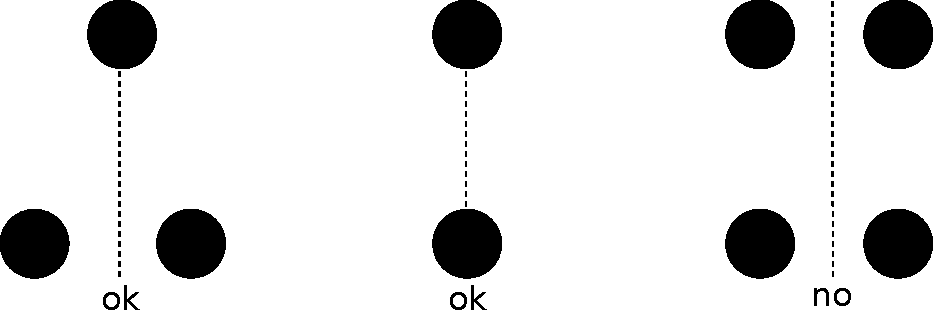
\includegraphics[scale=0.7]{images/n_48}
\end{center}

Nelle prime due immagini effettuare il Gathering è possibile, poichè abbiamo almeno un nodo su cui effettuarlo (quello tagliato dall'asse), nella terza invece è impossibile, non abbiamo nodi candidati su cui effettuare gathering.\\

\section{Risultati Positivi}
\theorem{Il Gathering è \textbf{risolvibile} se la configurazione iniziale è Asimmetrica e Aperiodica (Configurazione Rigida). In questi casi il problema del Gathering consiste nel riuscire a generare almeno una molteplicità.}
\begin{proof}
Assumiamo quindi che una molteplicità sia stata creata. Ai fini di far terminare la procedura di gathering si fa in modo che i robots che compongono la molteplicità non si muovano, mentre si fa in modo che tutti gli altri si avvicinino ad essa. Al più due a due la raggiungeranno finalizzando il gathering.
\end{proof}

\begin{itemize}
    \item Asimmetriche: La distanza che ha un robot dagli altri è diversa per tutti. Ovvero che nessun robot si può speacchiare con un altro robot dall'altra parte del ring.
    \item Aperiodiche: Non son presenti assi di simmetria.
\end{itemize}


La procedura, assumendo che una molteplicità sia stata creata per finalizzare il Gathering è la seguente:
\begin{itemize}
    \item Se R è in una molteplicità allora non si muove
    \item Altrimenti:
    \begin{itemize}
        \item Se il segmento che è presente tra te (Robot) ed R NON è libero allora non muoverti
        \item Altrimenti Muoviti verso la molteplicità tramite il più piccolo percorso libero oppure in caso di equità in qualsiasi percorso.
    \end{itemize}
\end{itemize}
\textbf{Lemma:} La procedura sopra descritta esegue il Gathering in una qualsiasi configurazione con una singola molteplicità.\\
\textbf{Dim:} Questo è vero perchè un robot si muove solamente se il segmento tra lui e la molteplicità è libero, ed in questo caso il robot si muove solamente sui nodi liberi del ring. Questo implica che nessun altra molteplicità oltre quella esistente verrà creata. Dato che per ogni configurazione con una singola molteplicità è garantito che alcuni robot abbiano un segmento vuoto tra loro e la molteplicità, ad un certo tempo $t$ questi robot andranno verso la molteplicità ed al più a due a due la raggiungeranno, facendo in modo che i segmenti si liberino per gli altri robot, che si muoveranno di conseguenza.

\section{Gathering nelle configurazioni Rigide:}
\subsection{Creazione di una singola molteplicità}
Abbiamo dedotto quindi che per finalizzare il gathering in qualsiasi configurazione rigida, indipendentemente dal numero di robots è necessario creare una singola molteplicità. \textbf{L'idea principale è quella di eleggere un singolo robot e muoverlo finchè non ne incontra un altro su un nodo, riuscendo quindi a creare una molteplicità e permettendo di finalizzare il gathering.} Fondamentale il fatto però che l'elezione di questo robot deve fare in modo che durante il suo cammino non crei una configurazione in cui il gathering non sia più risolvibile. Per far questo eleggiamo il robot nel seguente modo:\\

\textbf{Elezione del robot:} Quello che distingue i robot sono le distanze che hanno tra di loro. Da questa distanza posso ottenere due stringhe binarie analizzando entrambi le direzioni. Devo tenere conto di entrambe le direzioni perchè pur avendo la Asimmetria, dato che i robot non concordano sul verso, se uno computa la stringa a sinistra, ed un altro robot computa una stringa a desta è possibile che queste due siano uguali. Inserirò 0 se il nodo è vuoto, inserirò 1 se il nodo ha un robot sopra. (\textbf{Esempio:} 110111100). Ogni stringa calcolata sarà chiamata Vista. \\ Poiché la configurazione è asimmetrica necessariamente queste stringhe saranno tutte diverse, quindi è un po' come se i robot adesso avessero degli ID. Di queste due viste, un robot sceglie quella \textbf{minore}. Ogni robot può inoltre computare le stringhe di tutti gli altri durante la fase di Look.\\ \'E fondamentale poter distinguere i robot perchè così riusciamo a distinguere quello con vista minima, ovvero quella che ha il valore più piccolo. Questo robot sarà quello che è più vicino all'intervallo di nodi vuoti più lungo, e sarà lui il robot designato per effettuare lo spostamento. Questo avviene nella direzione OPPOSTA all'intervallo dei nodi vuoti e ora possono accadere due cose:
\begin{enumerate}
    \item Creiamo una molteplicità, e quindi il problema è risolto.
    \item Finiamo su un nodo vuoto, allargando quindi ulteriormente l'intervallo dei nodi vuoti
\end{enumerate}
Se ricadiamo sul secondo punto è necessario muovere nuovamente un altro robot, ma siamo sicuri che si muoverà sempre quello perchè la sua vista sarà ancora la più piccola di tutti, dato che avrà i bit ad 1 nelle posizioni \textbf{meno} significative della vista, mentre l'altro robot che sta nella parte opposta dell'intervallo dei nodi vuoti avrà gli 1 in posizioni più significative, e questo determina una grandezza maggiore della vista.

%A questo punto l'idea è:\\ Si prende l'intervallo di vuoti maggiore (ce ne può essere più di uno) e si considerano i due robot all'estremo di questo intervallo. A questo punto si fa muovere il robot con stringa minima (che sarà accanto alla serie più lunga di nodi vuoti) verso la parte OPPOSTA a quella con i nodi vuoti, così da allargare questo intervallo. Dopo questo passaggio la sequenza di vuoti maggiori è una sola (supponendo che prima ce ne fossero state di più). Adesso dovrò comunque scegliere tra due robot per effettuare lo spostamento, ma se al passo precedente ho scelto quello con la stringa minima, quest'ultimo nella nuova configurazione avrà stringa ancora più piccola di quella di prima, quindi si muoverà sempre lui riuscendo prima o poi a creare una molteplicità.



A questo punto \textbf{si muove il robot con vista minima rispetto a tutti perchè sarà accanto alla serie più lunga di nodi vuoti, e si muove verso la parte opposta a quella con i nodi vuoti, allargando ulteriormente questo intervallo.} Questo significa che al prossimo passo il robot che sarà elettro per lo spostamento sarà sempre lui, perchè ha comunque stringa più piccola di tutti. Si continua così fin quando non si crea la prima molteplicità e successivamente si applica la procedura per fare in modo che i nodi nella molteplicità non si muovano ed i restanti si muovano verso di essa.\\

\textbf{Idea:} Prendi l'intervallo di vuoti maggiore, scegli un estremo di questo intervallo e fai muovere il robot che ha stringa minore questo in maniera tale da allargare ulteriormente l'intervallo degli 0. Al passo successivo la sequenza di vuoti maggiori è una sola, dovrò scegliere eventualmente tra due nodi e se ho fatto la scelta opportuna continuerò a far muovere lo stesso robot, fino a quando non andrò a scontrarmi con un altro robot creando una molteplicità.\\
\textbf{Come garantisco che si muova sempre lo stesso robot?} Se io allargo da un estremo allora restringo dall'altro, e si muoverà quindi il robot con la stringa massima.
Poichè la configurazione è asimmetrica necessariamente queste stringhe saranno tutte diverse, ma ci potrebbero essere stringhe uguali perchè i robot non concordano su uno stesso verso. Quello che succede è che se uno legge una stringa in un verso e l'altro la legge dall'altro è possibile che le due stringhe siano uguali.\\
\textbf{Per ovviare a questo problema possiamo} fare in modo che ogni robot computa due stringhe, sia a destra che a sinistra, delle due ne sceglie una (quella più grande è più conveniente) e mette l'altra come suffisso (la mette davanti) così facendo tutte le stringhe saranno diverse. Ora possiamo effettivamente discriminare tra i vari robots. Nella fase di Look un robots può computare anche le stringhe di tutti gli altri, quindi dopo questa fase tutti sapranno quale sarà la stringa minima e quella massima nel Ring.\\
\textbf{Mi conviene far muovere il robot con la stringa maggiore}, che si muoverà sul robot limitrofo e creerà la molteplicità.

\textbf{Provo da Libro:} Supponiamo che i robot M ed N a distanza Max siano eletti per lo spostamento. Supponiamo che la distanza $a$ (la stringa) tra M ed M' sia minore della distanza $b$ tra N ed N'. Il robot M si muoverà verso il robot M'. Dopo questa mossa la distanza tra M ed N diventa Max + 1 e la distanza tra M ed M' diventa $a-1$. Nessun altra distanza viene modificata. La configurazione è ancora una volta rigida, perchè M ed N sono l'unica coppia di vicini a distanza Max+1 e la distanza $a-1$ tra M ed M' è pioù piccola della distanza $b$ tra N ed N'. I robot M ed N sono quindi nuovamente eletti perchè ora c'è solo un singolo vbicino a distanza b tra N ed N' e quindi sarà ancora il robot M che si muoverà verso M'. Ne segue che fino a quando una moltepclità non viene creata un solo robot alla volta si muoverà sempre nella stessa direzione.\\
In partenza la configurazione è asimmetrica, quindi di tutte le sequenze di vuoti massimali ne posso identificare una. Una volta individuata questa, sempre per la asimmetria posso individuare uno dei due estremi e se ho fatto la scelta opportuna muoverò sempre lo stesso robot, che è quello con la sequenza maggiore fin quando non creerò una molteplicità. Questo significa che se io allargo da un estremo allora restringo e si stringe fino a quando non viene creata una molteplicità Il protocollo da applicare potrebbe quindi essere quello di spostare il robot con la stringa massima. Questo pur muovendosi manterrà la stringa massima finchè non creerà una molteplicità. Da li in poi tutti gli altri robot possono unirsi a quella.

\theorem{
Se la configurazione è aperiodica ed ammette numero dispari di robot è possibile effettuare gathering
}
\begin{proof}
Essendo presente un numero dispari di robot, si avrà sicuramente una simmetria di tipo Arco-Nodo. La procedura consiste nel far muovere questo robot in una qualsiasi posizione adiacente, dimostreremo che tre casi possono accadere:
\begin{enumerate}
    \item Dopo lo spostamento si viene a creare una molteplicità. Succede quando il robot si sposta su un nodo dove era già presente un robot. Essendo presente una molteplicità allora è possibile finalizzare il gathering per il teorema precedente.
    \item La configurazione successiva è rigida (Asimmetrica e Aperiodica). A questo punto per il teorema precedente il gathering è risolvibile (il Th è quello delle stringhe Max).
    \item Si viene a creare un altro asse di simmetria (quello precedente è stato eliminato dallo spostamento del nodo sull'asse). In questo caso la simmetria diventa per forza di tipo Nodo-Arco. Si muove quindi il robot nell'asse di simmetria in un qualsiasi nodo adiacente, così facendo si ricadrà su uno di questi tre punti, riuscendo a finalizzare il gathering prima o poi. In un numero finito di passi la configurazione o diventa rigida oppure si crea una molteplicità [Non dimostrato].
\end{enumerate}
\end{proof}
L'algoritmo per far questo è il seguente:
\textbf{Odd-Gathering:}
\begin{itemize}
    \item Se la configurazione è periodica allora il Gathering è impossibile
    \item Altrimenti:
    \begin{itemize}
        \item Se la configurazione possiede una singola molteplicità allora applica Single-Multiplicity-Gathering.
        \item Altrimenti se la configurazione è rigida applica il Th sopra difficilissimo
        \item Altrimenti muovi il robot sull'asse di simmetria in un qualsiasi nodo adiacente.
    \end{itemize}
\end{itemize}

\section{Gathering in altri sistemi}
Nel precedente articolo abbiamo visto il gathering su sistemi Asincroni, ovvero che la durata di ogni ciclo di LCM può durare in maniera diversa per ogni robot. Può succedere quindi che un robot si svegli, effettui la Look e nello stesso momento si sveglia un altro robot che effettua un ciclo completo di LCM prima che il primo robot effettui la Compute. Questo poteva creare dei problemi, poichè, nell'esatto caso sopra descritto, il primo robot effettuerà la sua Move su una foto \textbf{obsoleta} del sistema. Vediamo quindi cosa succede con altri sistemi:\\
\textbf{Modello Fully Synchronous (FSYNC):} Ogni ciclo di LCM ha la stessa durata per ogni robot; la mossa avverà esattamente dopo n cicli di clock e per tutti i robot, poichè si svegliano tutti allo stesso momento.\\
Riassumendo, in questo modello avremo:\\
|L|C|M|L|C|M|L|C|M|\\
|L|C|M|L|C|M|L|C|M|\\
|L|C|M|L|C|M|L|C|M|\\
per tutti i robot.\\
\textbf{Modello Semi Synchronous (SSYNC):} Non tutti i robot si svegliano subito, la durata di LCM è la stessa per tutti. In questo caso avremo:\\\\
|L|C|M|L|C|M|\\
|-|-|-|L|C|M|\\
|L|C|M|-|-|-|\\
\textbf{Vediamo alcuni esempi di problemi risolvibili in questo modello e NON nel modello FSYNC:}\\
Prendiamo ad esempio, in questo modello, un Ring con un numero dispari di nodi e posizioniamo esattamente due robot. Ovunque li mettiamo la configurazione sarà simmetrica nodo-arco. Dato il modello in cui siamo (SSYNC), abbiamo la certezza che prima o poi entrambi si sveglieranno. Nel ciclo di LCM scelgo un nodo e tutti si muoveranno verso il nodo scelto come finalizzatore del gathering, quindi in questi sistemi è risolvibile. Nel mondo Asincrono questo non sarebbe possibile, poichè se ne sposterebbe solo uno alla volta, e l'avversario potrebbe fare in modo che l'esecuzione sia speculare, non finalizzando ma il gathering.\\
Possiamo parlare di una gerarchia tra i livelli: \textbf{FSYNC $>$ SSYNC}, due robot gatherabili nel mondo FSYNC sono gatherabili anche nel mondo SSYNC ma non vale il viceversa (vedi esempio sopra).\\
\section{Ritorno al mondo Asincrono}
Il gathering nel mondo ASYNC si è dimostrato risolubile per tutte le seguenti configurazioni:
\begin{itemize}
    \item Aperiodiche
    \item Simmetriche ma non Arco-Arco
    \item Numero di robot maggiore di 2
    \item Configurazioni non appartenenti a SP4 (Special Four).
\end{itemize}
\textbf{Cosa sono le configurazioni SP4?} Le caratteristiche di queste configurazioni sono le seguenti:
\begin{itemize}
    \item Simmetriche di tipo nodo-arco.
    \item Sono sempre presenti quattro robot.
    \item Ring Dispari. (Viene in automatico dai due punti precedenti)
\end{itemize}{}
Nell'esempio sul quaderno, considerando i due intervalli di nodi "liberi", ovvero dove non sono presenti robot, su cui passa l'asse di simmetria, l'intervallo di nodi Dispari è maggiore di quelli dei nodi Pari.\\
\textbf{Gathering SP4 su 5 nodi su FSYNC:}\\
Prendiamo ad esempio la più piccola SP4 possibile, il disegno è su quaderno. Nel mondo asincrono le mosse sono:
\begin{itemize}
    \item I robot vicini al nodo vuoto si devono muovere verso il medesimo, ma l'avversario non li sveglierà entrambi, ma solo 1 e lo sposta, facendo spostare di conseguenza l'asse di simmetria. La configurazione diventa periodica e non è possibile finalizzare il gathering.
    \item L'avversario crea 2 molteplicità mandando i robot uno sopra l'altro ed il gathering non è risolubile perchè si crea una configurazione periodica.
    \item Uguale alla precedente ma con l'altra coppia di nodi.
    \item Mossa di Swap tra i 4 nodi aventi il robot sopra, si crea sempre la stessa configurazione.
\end{itemize}
Come possiamo notare dai quattro punti precedenti, per ogni mossa c'è sempre una contromossa dell'avversario che fa fallire il protocollo. Si conclude che il gathering nelle SP4 su 5 nodi non è risolubile.\\
\textbf{Gathering SP4 su 7 nodi su FSYNC:} Non risolvibile, esempi sul quaderno viola di carpi.
\textbf{Gathering SP4 su 9 nodi su FSYNC:} Non risolvibile.
Nello specifico, c'è una determinata configurazione (posizionamento di robot sui nodi) che crea un sacco di problemi, per provare tutte le possibili opzioni di posizionamento ci si mette un tempo lunghissimo.\\ La difficoltà principale del mondo FSYNC è che dato che l'avversario può spostare un nodo alla volta può variare facilmente l'asse di simmetria non permettendo la finalizzazione del gathering.
\section{Mondo SSYNC (Semisincrono)}
\textbf{ Le SP4 su mondo semisincrono sono risolubili tranne la SP4 su 5 nodi.}
In questo mondo sono risolvibili perchè non esistono alcune configurazioni che sono esattamente quelle che danno problemi nel mondo del FSYNC, ovvero quelle che fanno sovrapporre le mosse di Look e Move.\\
\section{Robot su piano euclideo}
Il gathering è risolvibile in questi sistemi per un numero di robot maggiore di 2. Sono visti in questo caso come punti del piano.\\ \textbf{Smallest Enclosing Circle:} Un robot si sveglia, fa la foto della configurazione e deve computare il cerchio più piccolo possibile che contiene tutti i punti. Questo cerchio sarà unico, ne segue quindi che anche il suo centro sarà unico; i robot finalizzeranno il gathering proprio nel centro. Le mosse quindi vanno effettuate in maniera tale da non far spostare il centro del cerchio.\\
\properties{ I punti fondamentali che determinano il cerchio o sono due sul diametro oppure sono 3 robot.} 
In sostanza questa proprità dice di non far muovere i robot che potrebbero spostare il centro. Supponiamo tutti i robot posizionati sul diametro perfettamente stabili, essi avranno tutti la stessa vista e quindi la mossa la possono fare tutti, in questa configurazioni non è possibile lasciare 3 robot o 2 sul diametro, l'unica soluzione è muoverli tutti assieme verso il centro. Siamo però in un sistema asincorno, quindi non tutti si svegliano insieme.

